\documentclass[lettersize,journal]{IEEEtran}
\usepackage{amsmath,amsfonts}
%\usepackage{algorithmic}
%\usepackage{algorithm}
\usepackage[ruled,vlined,linesnumbered,ruled]{algorithm2e}
\usepackage{array}
\usepackage[caption=false,font=normalsize,labelfont=sf,textfont=sf]{subfig}
\usepackage{textcomp}
\usepackage{stfloats}
\usepackage{url}
\usepackage{verbatim}
\usepackage{graphicx}
\usepackage{cite}
\hyphenation{op-tical net-works semi-conduc-tor IEEE-Xplore}
% updated with editorial comments 8/9/2021

\usepackage{makecell}
\usepackage{multirow}
\usepackage{siunitx} 
\usepackage{amssymb}
%\usepackage[ruled]{algorithm2e}
\usepackage{algorithmic}
\usepackage{amsthm}
\usepackage{bm}
\usepackage{booktabs}
\usepackage{colortbl}
\usepackage{ragged2e}

\usepackage{color}

\newtheorem{theorem}{Theorem}
\newcommand{\qedblacksquare}{\hfill $\blacksquare$}

\begin{document}

\title{A Crosstalk Suppression Scheme Utilizing the Dynamic Shielding and Bit-Stuffing Code for Hexagonal TSV Arrays}

\author{Chen~Wei,
	Huan Yang, 
	Xiaole~Cui,~\IEEEmembership{Member,~IEEE}, 
	and Xing~Zhang
	% <-this % stops a space
	
\thanks{Manuscript received XX XX 2025. This work was supported by the National Natural Science Foundation of China (NSFC) under Grant No. 92373206, the National Key Research and Development Program of Ministry of Science and Technology under Grant No. 2024YFB3614200, the Guangdong Provincial Key Lab of In-Memory Computing Chips	under Grants No. 2024B1212020002, the Shenzhen Science and Technology Program under Grants No. JCYJ20220818100814033, No. SGDX20230116093303006, No. KJZD20231023100201003 and No. KQTD20200820113105004. \textit{(Corresponding author: Xiaole Cui.)}}% <-this % stops a space
\thanks{The authors are with Peking University Shenzhen Graduate School, Shenzhen 518055 China (e-mail: iris.cw@outlook.com; hypku324@sina.com; cuixl@pkusz.edu.cn; zhx@pku.edu.cn).}% <-this % stops a space
}

% The paper headers
\markboth{IEEE Transactions on Computer-Aided Design of Integrated Circuits and Systems,~Vol.~1, No.~1, October~2025}%
{Shell \MakeLowercase{\textit{Wei et al.}}: A Crosstalk Suppression Scheme Utilizing the Dynamic Shielding and Bit-Stuffing Code for Hexagonal TSV arrays}

%\IEEEpubid{0000--0000/00\$00.00~\copyright~2021 IEEE}
% Remember, if you use this you must call \IEEEpubidadjcol in the second
% column for its text to clear the IEEEpubid mark.

\maketitle

\begin{abstract}
The through silicon via (TSV) arrays play the role of vertical electrical interconnections in the chiplet-based integrated circuits. The hexagonal array achieves a higher TSV density than the rectangular array, but it suffers more severe inter-TSV crosstalk which increases the interconnection delay and deteriorates the signal integrity. Researchers have proposed many crosstalk suppression schemes based on the shielding and crosstalk avoidance code (CAC) techniques, but most of them are applicable only to the rectangular arrays. This paper proposes a crosstalk suppression scheme utilizing the dynamic shielding and bit-stuffing code techniques for hexagonal TSV arrays. Firstly, a novel dynamic shielding scheme is proposed to reduce the maximum crosstalk of the signal TSVs in hexagonal arrays. Then, the bit-stuffing CAC (BS-CAC) is proposed to eliminate the data patterns which cause the high-level crosstalk when these patterns are transmitted through TSVs. The analysis and simulation show that the proposed scheme is able to reduce the inter-TSV crosstalk in hexagonal arrays by 4C-level with the bit overhead of less than 51.5\%, and the hardware overhead is less than the existing FTF/FPF-CAC methods. 
 
\end{abstract}

\begin{IEEEkeywords}
Bit-stuffing code, crosstalk avoidance code (CAC), dynamic shielding, through silicon via (TSV).
\end{IEEEkeywords}

\section{Introduction}\label{sec-intro}
\IEEEPARstart{T}{he} 2.5D/3D integration is regarded as one of the feasible solutions for the chiplet-based integrated circuits. It has advantages including the high integration density, the elongated global interconnects and the heterogeneous fabrication process, which address the challenges of the post Moore’s law era. In chiplet-based integrated circuits, the stacked bare dies are often connected vertically by the through silicon vias (TSVs). In practice, the clustered TSVs are usually organized as the rectangular or hexagonal TSV arrays to regulate the routing rules \cite{A04_Vaisband_7448908}.

In TSV arrays, the significant capacitive couplings between the adjacent TSVs occur due to the large TSV dimension and the tight spacing \cite{A05_Kumar_6513784}. This effect results in the non-negligible coupling crosstalk between the closely clustered TSVs, which deteriorates the signal integrity and increases the interconnection delay \cite{A07_Song_7273940}. 

The methods to reduce the maximum crosstalk in TSV arrays can be classified into physical methods, shielding methods and CAC methods. Increasing TSV spacing is the most typical physical method to reduce the inter-TSV crosstalk \cite{A09_Kim_5699376}. However, subsequent research revealed that the practical effect of this approach is not as good as expected \cite{A07_Song_7273940}. The severity of crosstalk is related to the signal patterns transmitted through the TSV arrays \cite{A05_Kumar_6513784,A07_Song_7273940,A10_Cui_7851080,A11_Cui_9509749}. By avoiding the patterns which result in the worst crosstalk cases, the shielding methods \cite{A12_Hu_7517149,A13_Mei_8480511,A14_Cui_8480772,A15_Chang_6509678} and the crosstalk avoidance code (CAC) methods \cite{A05_Kumar_6513784,A10_Cui_7851080,A11_Cui_9509749,A16_Wu_5395631,A17_Shirmohammadi_6675266,A18_Shirmohammadi_7780349,A19_Zou_6742982,A20_Ran_7588317,A21_Wei_10224770,A22_Wei_9796564} are able to reduce the maximum crosstalk level, thereby improving the signal integrity in TSV arrays. The shielding and CAC methods are not in conflict with the physical methods, and they can effectively decrease the severity of crosstalk in the array with determined physical parameters. The CAC methods are of great concern, because the existing studies have indicated that the optimal bit overhead of the static shielding scheme is highly likely to be inferior to that of the CAC scheme \cite{A14_Cui_8480772,A23_Luo_8126413}. Nevertheless, the shielding techniques are employed to reduce the complexity of the codec design or achieve a higher crosstalk suppression capability in some CAC schemes \cite{A11_Cui_9509749,A20_Ran_7588317}.

The hexagonal arrays have a completely symmetric topology, in which each TSV requires 13\% less area than that in rectangular arrays, and this makes the hexagonal array a better choice than the rectangular array in many scenarios \cite{A04_Vaisband_7448908}. However, higher TSV density leads to a more severe inter-TSV crosstalk and brings much more difficulties in the crosstalk suppression scheme design. Unfortunately, most of the existing crosstalk suppression methods are designed for the rectangular arrays, which cannot be applied to the hexagonal arrays.

This work proposes a crosstalk suppression scheme utilizing the dynamic shielding and bit-stuffing code techniques for the hexagonal TSV arrays. The rest of this paper is organized as follows. Firstly, Section \ref{sec-pre} introduces the crosstalk model in TSV arrays, discusses the existing crosstalk suppression schemes and presents the motivation of this work. Secondly, a novel dynamic shielding scheme is proposed in Section \ref{sec-dysh}. By setting the TSVs at specific locations as the dynamic shielding TSVs which have a low transmission frequency, the maximum crosstalk suffered by the signal TSVs can be reduced by 2C level. Thirdly, based on the dynamic shielding scheme proposed in Section \ref{sec-dysh}, the bit-stuffing CAC (BS-CAC) scheme is put forward in Section \ref{sec-bscac}. By combining the proposed dynamic shielding scheme and CAC scheme, the maximum crosstalk suffered by the signal TSVs can be reduced by 4C level. Then, Section \ref{sec-code_rate} analyzes the code efficiency of the proposed scheme. Next, Section \ref{sec-simu} validates the superiority of the proposed scheme over the existing methods in terms of the crosstalk suppression capability, bit overhead, and hardware overhead through simulation results. Finally, Section \ref{sec-conclusion} concludes this paper.


\section{Related Works and Motivations}\label{sec-pre}
\subsection{The coupling crosstalk in TSV arrays}\label{subsec-pre-xtalkModel}
In TSV arrays, the coupling crosstalk suffered by each victim TSV comes almost from the aggressor TSVs that are topologically adjacent to it \cite{A04_Vaisband_7448908,A05_Kumar_6513784}. As shown in Fig. \ref{fig-TSVArrays}(a), the victim $\rm TSV_A$ in a rectangular array has up to four directly adjacent aggressor TSVs ($\rm TSV_C$, $\rm TSV_E$, $\rm TSV_F$, $\rm TSV_H$) and up to four diagonally adjacent aggressor TSVs ($\rm TSV_B$, $\rm TSV_D$, $\rm TSV_G$, $\rm TSV_I$). For the victim $\rm TSV_A$ in a hexagonal array, as shown in Fig. \ref{fig-TSVArrays}(b), there are up to six directly adjacent aggressor TSVs ($\rm TSV_B$, $\rm TSV_C$, $\rm TSV_D$, $\rm TSV_E$, $\rm TSV_F$, $\rm TSV_G$). The crosstalk severity suffered by the victim $\rm TSV_A$ in Fig. \ref{fig-TSVArrays} can be quantified by the formula (\ref{eq-xtalk_level_calc}) \cite{A04_Vaisband_7448908,A05_Kumar_6513784,A07_Song_7273940,A10_Cui_7851080}.

\begin{figure}[t]
	\centering
	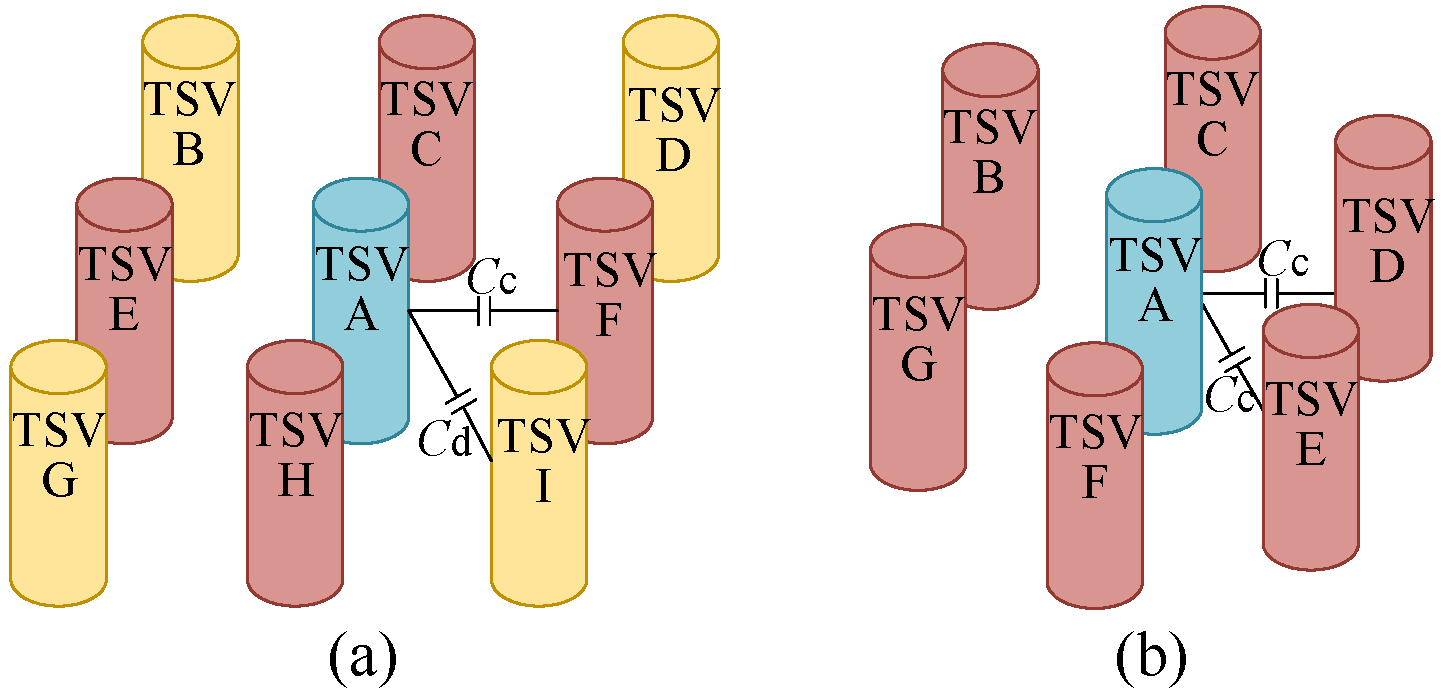
\includegraphics[width=2.3in]{./fig_files/TSVArray.pdf}
	\caption{The TSV arrays in which the victim $\rm TSV_A$ suffers the coupling crosstalk from its adjacent aggressor TSVs. (a) The rectangular TSV array; (b) The hexagonal TSV array.}
	\label{fig-TSVArrays}
\end{figure}

\begin{equation}
	\begin{aligned}
		{C_{\rm eff, TSV_A}} = &\\
		C_{\rm L}(1+&\sum_{{\rm TSV}_i\in {\rm Adj(TSV_A)}}^{}{(\lambda_{{\rm TSV}_{\rm A},{\rm TSV}_{i}} \delta_{{\rm TSV}_{\rm A},{\rm TSV}_{i}})}) 
	\end{aligned}
	\label{eq-xtalk_level_calc}
\end{equation}

In formula (\ref{eq-xtalk_level_calc}), $C_{\rm L}$ represents the load capacitance of $\rm TSV_A$. $\rm Adj(TSV_A)$ is the set of TSVs that are topologically adjacent to $\rm TSV_A$. Specifically, for the $\rm TSV_A$ in Fig. \ref{fig-TSVArrays}(a), $\rm Adj(TSV_A)$ is \{$\rm TSV_B$, $\rm TSV_C$, $\rm TSV_D$, $\rm TSV_E$, $\rm TSV_F$, $\rm TSV_G$, $\rm TSV_H$, $\rm TSV_I$\}. For the $\rm TSV_A$ in Fig. \ref{fig-TSVArrays}(b), $\rm Adj(TSV_A)$ is \{$\rm TSV_B$, $\rm TSV_C$, $\rm TSV_D$, $\rm TSV_E$, $\rm TSV_F$, $\rm TSV_G$\}. For each ${\rm TSV}_i$ in the $\rm Adj(TSV_A )$ set, the variable $\lambda_{{\rm TSV_A},{\rm TSV}_i}$ is the ratio of the coupling capacitance between $\rm TSV_A$ and ${\rm TSV}_i$ to the load capacitance $C_{\rm L}$. Assume that the $\rm TSV_A$ is a non-edge TSV, i.e., $\rm TSV_A$ is not located at the edge of the array. For a specific array, the value of  $\lambda_{{\rm TSV_A},{\rm TSV}_i}$ is regarded as a fixed value which is denoted as $\lambda$ if ${\rm TSV}_i$ is directly adjacent to $\rm TSV_A$. If ${\rm TSV}_i$ is diagonally adjacent to $\rm TSV_A$, the value of  $\lambda_{{\rm TSV_A},{\rm TSV}_i}$ is approximately equal to $\lambda/4$ \cite{A05_Kumar_6513784}. 

The variable $\delta_{{\rm TSV_A},{\rm TSV}_i}\in \{0,1,2\}$ in formula (\ref{eq-xtalk_level_calc}) indicates the relative transition state of the signals on $\rm TSV_A$ and ${\rm TSV}_i$. The value of $\delta_{{\rm TSV_A},{\rm TSV}_i}$ is 2 if the opposite signal transitions occur on $\rm TSV_A$ and ${\rm TSV}_i$. The value of $\delta_{{\rm TSV_A},{\rm TSV}_i}$ is 1 if only one of the signals on $\rm TSV_A$ and ${\rm TSV}_i$ has a transition. The value of $\delta_{{\rm TSV_A},{\rm TSV}_i}$ is 0 if the same transitions occur on $\rm TSV_A$ and ${\rm TSV}_i$ or neither of these two TSVs has a transition. Depending on the data patterns transmitted through the TSVs, each directly adjacent aggressor TSV may result in the crosstalk of $0\lambda C_{\rm L}$, $1\lambda C_{\rm L}$ or $2\lambda C_{\rm L}$ level to the victim TSV, and each diagonally adjacent aggressor TSV may result in the crosstalk of $0\lambda C_{\rm L}$, $0.25\lambda C_{\rm L}$ or  $0.5\lambda C_{\rm L}$ level to the victim TSV. Therefore, the crosstalk level suffered by the non-edge TSVs in rectangular arrays ranges from $C_{\rm L}$ to $C_{\rm L}+10\lambda C_{\rm L}$, and the crosstalk level suffered by the TSVs in hexagonal arrays ranges from $C_{\rm L}$ to $C_{\rm L}+12\lambda C_{\rm L}$. 

If the victim $\rm TSV_A$ is located at the edge of TSV array, the maximum crosstalk level it suffers is almost the same as that of the non-edge TSVs due to the edge effect, even if the edge TSV has less aggressors than the non-edge TSVs \cite{A24_Bamberg_8106994,A25_BAMBERG201998}. In this paper, the crosstalk level $C_{\rm L}+n\lambda C_{\rm L}$ in the TSV array is abbreviated as $n$C. A crosstalk suppression solution is referred to as the $n$C-reduction scheme for a specific type of TSV arrays, if it reduces the maximum crosstalk in these TSV arrays by $n\lambda C_{\rm L}$.

\subsection{The existing crosstalk suppression schemes for TSV arrays}\label{subsec-pre-relatedWorks}
The static shielding, which connects some TSVs to the power supply or ground, is effective in reducing the crosstalk suffered by the remaining signal TSVs. The objective of the static shielding scheme is to minimize the bit overhead, i.e., employ the least number of shielding TSVs to guarantee that the crosstalk levels on all signal TSVs do not exceed a given threshold. Hu et al. \cite{A12_Hu_7517149} used the re-layout and static shielding techniques to reduce the inter-TSV crosstalk. Mei et al. \cite{A13_Mei_8480511} proposed an interleaving layout method, which limits the inter-TSV crosstalk to a very low level with a large proportion of shielding TSVs. The exhaustive search is an approach to get the optimal static shielding scheme for the given TSV array and crosstalk threshold \cite{A14_Cui_8480772}. However, exhaustive search is not applicable for the large-scale arrays because of the prohibitive computation complexity. Even in the small-scale arrays, the existing studies have indicated that the optimal bit overhead of the static shielding scheme is highly likely to be inferior to that of the CAC scheme. Chang et al. \cite{A15_Chang_6509678} proposed a novel concept distinct from the static shielding, which is referred to as the dynamic shielding. This method remaps the less transitional data bits during a period to the TSVs as temporary shielding wires. Unlike the static shielding which connects the TSV to power supply or ground, the dynamic shielding wires are still signal TSVs for data transmission, but with the highly constrained switching activity. Although the method in \cite{A15_Chang_6509678} is more flexible than the static shielding methods, it requires a very complex controller.

The CAC methods are of great concern, because their bit overhead is usually lower. Kumar et al. \cite{A05_Kumar_6513784} applied the Fibonacci numeral system based CAC (FNS-CAC) into the rectangular TSV array row by row to suppress the inter-TSV crosstalk from 10C level to 8C level. Wu et al. \cite{A16_Wu_5395631} proposed the modified Fibonacci numeral system (MFNS) by redefining the largest number of the FNS sequence. The MFNS-based CAC (MFNS-CAC) has a smaller bit overhead than FNS-CAC. Shirmohammadi et al. \cite{A17_Shirmohammadi_6675266,A18_Shirmohammadi_7780349} proposed the IDP-Fibo numeral system based CAC and the 3D-DPS-CAC algorithms, which have smaller bit overhead than FNS-CAC when they are applied in the rectangular arrays. Zou et al. \cite{A19_Zou_6742982} proposed the 3D-LAT scheme, which is the extension of the less adjacent transition (LAT) code for 2D buses, to avoid the worst crosstalk cases in rectangular TSV arrays by limiting the signal transition in each transmission cycle. Ran et al. \cite{A20_Ran_7588317} reduced the inter-TSV crosstalk in the three-row array to 4.5C level by combining the FNS-CAC and the static shielding. Cui et al. \cite{A10_Cui_7851080} reduced the bit overhead of applying FNS-CAC technique in three-row rectangular array to about 50\%, by utilizing the redundancies of FNS-CAC codewords. The 3D-DyCAC method is able to decrease the crosstalk noise to 7.5C level with at least 71\% bit overhead by considering the dynamic data transitions. Cui et al. \cite{A11_Cui_9509749} proposed the Mosaic-3C1S scheme which combines the static shielding technique with the triangular numeral system (TNS) based CAC algorithm. The Mosaic-3C1S scheme suppresses the inter-TSV crosstalk to 6C level with a bit overhead of only 25\%$\sim$45\%. Wei et al. \cite{FNSCATF_10945736} designed the FNS-based cyclic adjacent transition free CAC (FNS-CATF-CAC) for the large-size rectangular and hexagonal TSV arrays, which achieves a lower hardware overhead than the traditional FNS-CAC schemes. However, it reduces the inter-TSV crosstalk by only 2.5C level to 3C level, and its bit overhead is no less than that of the FPF-CAC and FTF-CAC schemes.


\subsection{Motivations}\label{subsec-pre-motications}
%The higher TSV density of hexagonal TSV array leads to a higher crosstalk level, which makes the crosstalk suppression in hexagonal TSV arrays more urgent. As discussed in Part \ref{subsec-pre-xtalkModel}, the maximum crosstalk level suffered by the TSVs in a hexagonal array is 2C larger than that in a rectangular array, which brings a more serious challenge to the reliable signal transmission. 

The design of the crosstalk suppression scheme for hexagonal array is a much more challenging task than that for rectangular array. Although each TSV in the rectangular array has up to eight adjacent TSVs, half of them are the diagonally adjacent aggressors. The maximum crosstalk brought by a diagonally adjacent aggressor is only one quarter of that by a directly adjacent aggressor according to Part \ref{subsec-pre-xtalkModel}. Therefore, for the crosstalk suppression schemes designed for rectangular arrays, it is usually sufficient to suppress the maximum crosstalk in the array only by restricting the crosstalk between the victim TSV and its four directly adjacent aggressors. However, in the hexagonal arrays, each victim TSV has up to six directly adjacent aggressors, and the crosstalk suppression schemes need to consider all these aggressors equally. 

As stated in Part \ref{subsec-pre-relatedWorks}, there are many shielding and CAC schemes for reducing the crosstalk level. Most of them are designed specifically for the rectangular arrays. The FTF-CAC and FPF-CAC schemes with row-by-row mapping, together with the FNS-CATF method, are among the few existing methods that can be directly applied to hexagonal arrays. However, they have some drawbacks as follows. 

(1)	The FTF/FPF-CAC method and the FNS-CATF method can reduce the maximum crosstalk in hexagonal arrays from 12C level to 10C level and 9C level, respectively. Considering the higher crosstalk severity in hexagonal arrays, this is not sufficient in many cases. In addition, the crosstalk effects on the edge TSVs are ignored in the existing FTF/FPF-CAC methods. This makes the practical crosstalk level suffered by the edge TSVs exceed the expectation.

(2)	The FTF/FPF-CAC method has a bit overhead of about 45\%, which is manifestly excessive for a 2C-reduction scheme. The bit overhead of FNS-CATF method is no less than that of the FTF/FPF-CAC method. 
 
(3)	Most of the existing research focuses on the combination of CAC and static shielding techniques. The possibility of the joint application of CAC and dynamic shielding techniques have not been explored. 


\section{The Optimal 2C-Reduction Dynamic Shielding Scheme for Hexagonal TSV Arrays}\label{sec-dysh}
\subsection{The proposed dynamic shielding technique}\label{subsec-dysh-intro}
In the proposed dynamic shielding scheme, the TSVs in a hexagonal array are classified into the following two types.

{\bf (1) Signal TSVs (STSVs):} It takes one transmission cycle to transmit 1-bit data through an STSV.

{\bf (2) Dynamic shielding TSVs (DTSVs):} Transmitting 1-bit data on a DTSV requires $r$ consecutive transmission cycles, in which $r\geq 2$. A DTSV is in one of the following two states in each transmission cycle. {\bf (a) Shielding state:} The signal on the DTSV in the shielding state remains unchanged. {\bf (b) Non-shielding state:} The signal on a DTSV is able to transit only if this DTSV is in the non-shielding state. The transmission cycles in which a DTSV is in the shielding state are referred to as the {\bf shielding cycles} of this DTSV, and the transmission cycles in which a DTSV is in the non-shielding state are referred to as the {\bf non-shielding cycles} of this DTSV.

Fig. \ref{fig-dysh_intro} presents an example of the DTSVs in a TSV array. Fig. \ref{fig-dysh_intro}(a) shows the array topology, where twelve STSVs are marked in blue and two DTSVs (D1 and D2) are marked in black. Fig. \ref{fig-dysh_intro}(b) presents the timing diagram, in which CLK is the clock signal. For the convenience of description, the green numbers are used to distinguish the different transmission cycles in Fig. \ref{fig-dysh_intro}(b). In this example, it takes two consecutive transmission cycles for D1 or D2 to transmit 1-bit data. The signal on D1 can only change in the cycles with odd numbers and remain invariant in those with even numbers. The signal on D2 can only change in the cycles with even numbers and remain invariant in those with odd numbersycles of D2 encompass and exclusively consist of all the cycles with odd numbers. The STSVs transmit data in each cycle.

\begin{figure}[t]
	\centering
	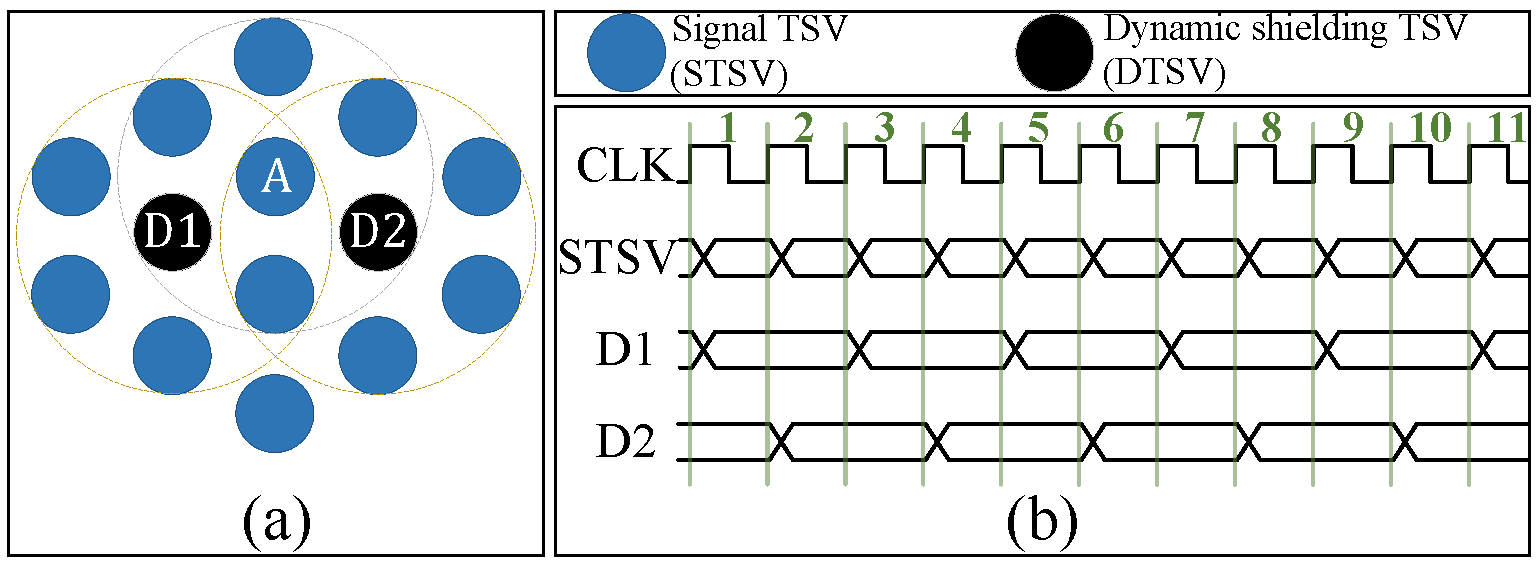
\includegraphics[width=2.7in]{./fig_files/dysh_intro.pdf}
	\caption{A hexagonal TSV array with twelve signal TSVs and two dynamic shielding TSVs. (a) The array topology. (b) The timing diagram of the data on TSVs.}
	\label{fig-dysh_intro}
\end{figure}

For each DTSV, the maximum crosstalk level imposed on its directly adjacent TSVs is 2C within its non-shielding cycles, which is equal to the maximum crosstalk level between two directly adjacent STSVs. However, the maximum crosstalk level a DTSV imposes on its directly adjacent TSVs is only 1C during its shielding cycles, because the signal on a DTSV remains unchanged in its shielding cycles. Take the STSV A which is directly adjacent to the DTSVs D1 and D2 in Fig. \ref{fig-dysh_intro} as an example. In the shielding cycles of D1, the maximum crosstalk level suffered by STSV A from D1 is 1C, while that from each adjacent TSV other than D1 is 2C. In the shielding cycles of D2, the maximum crosstalk level suffered by STSV A from D2 is 1C, while that from each adjacent TSV other than D2 is 2C. Each cycle is either a shielding cycle of D1 or a shielding cycle of D2, so the maximum crosstalk that STSV A suffers never exceeds 11C level. The DTSVs are insensitive to the crosstalk, because each data bit transmitted through them occupies consecutive multiple cycles, which is enough to stabilize the high-delay transition signal.

In this paper, the DTSVs with exactly the same shielding cycles are defined as being of the same type. A TSV array typically comprises multiple types of DTSVs. The D1 and D2 in Fig. \ref{fig-dysh_intro} are two distinct types of DTSVs. 


\subsection{Optimization of the dynamic shielding layout}\label{subsec-dysh-layout}
By setting more TSVs as DTSVs, the crosstalk suffered by STSVs in the array is expected to be reduced. However, the data transmission efficiency is also reduced, because the signal transmission frequency of DTSVs is lower than that of STSVs. Therefore, it is essential to optimize the layout scheme of the DTSVs to minimize their number, subject to the constraint that the maximum crosstalk experienced by each STSV does not exceed a specified level.
An optimal layout scheme should satisfy the following guidance as far as possible.

{\bf Guidance (1):} All the non-edge STSVs (i.e., the STSVs not located at the edge of an array) have the same type and quantity of directly adjacent DTSVs. Because an optimal layout scheme is expected to evenly distribute the crosstalk suppression effect of DTSV to each STSV, rather than making the crosstalk of some STSV significantly lower than that of the others.

{\bf Guidance (2):} No directly adjacent DTSVs. This prevents the waste of the crosstalk reduction effect of a DTSV on another DTSV.

{\bf Guidance (3):} For each STSV, the number of its directly adjacent DTSVs that are in the shielding cycle is the same in different transmission cycles. This prevents the maximum crosstalk level of a non-edge STSV from being higher in some cycles than in the other cycles.

The above guidances are the optimization advice rather than the indispensable conditions. Fig. \ref{fig-dysh_layout} presents an optimal dynamic shielding layout scheme that satisfies all the above guidances. This optimal layout scheme is able to reduce the maximum crosstalk suffered by each STSV from 12C to 10C. As shown in Fig. \ref{fig-dysh_layout}(a), there are three types of DTSVs which are denoted as D1, D2 and D3 respectively. The timing diagrams of these DTSVs are shown in Fig. \ref{fig-dysh_layout}(b). The 1-bit data transmission on each DTSV occupies three consecutive transmission cycles. As shown in Fig. \ref{fig-dysh_layout}(c)$\sim$(e), each STSV in Fig. \ref{fig-dysh_layout}(a) is directly adjacent to three DTSVs, and all the six directly adjacent TSVs of each DTSV are STSVs. For any STSV in Fig. \ref{fig-dysh_layout}(a), there are exactly two adjacent DTSVs in the shielding state. Therefore, the maximum crosstalk an STSV is 10C according to the discussion in Part \ref{subsec-dysh-intro}.

\begin{figure}[t]
	\centering
	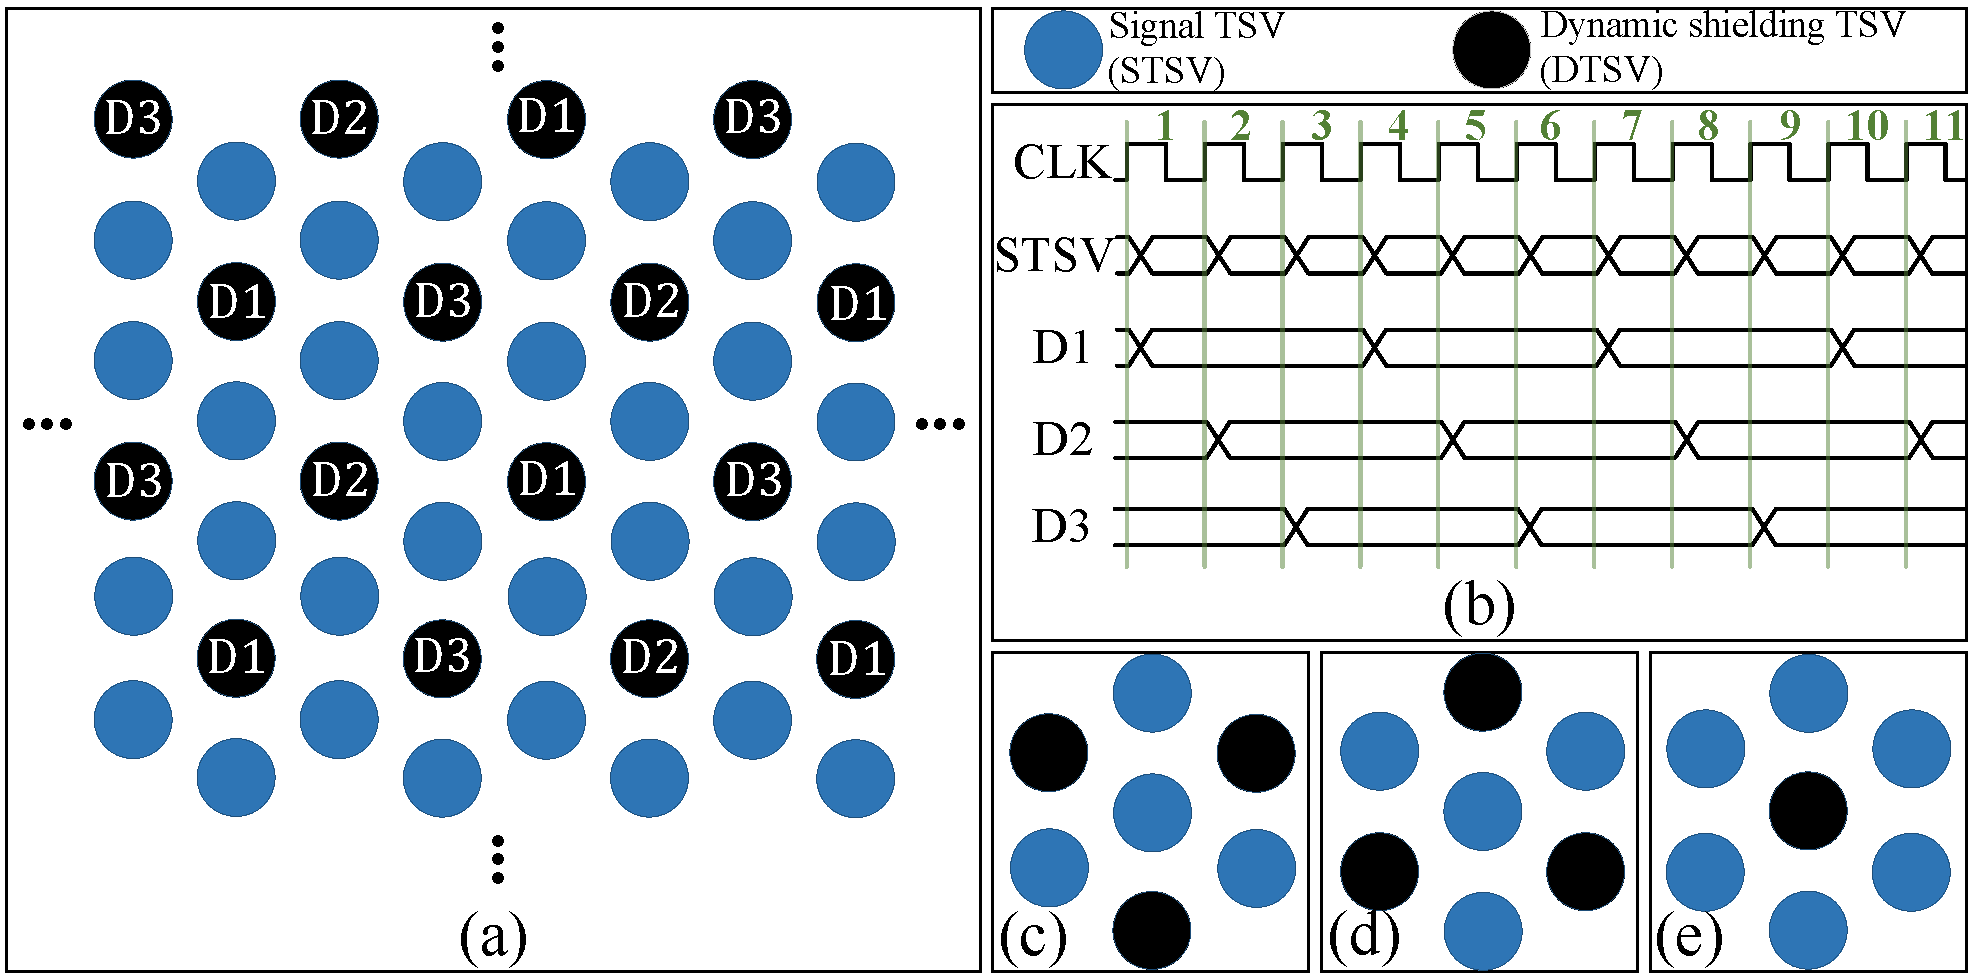
\includegraphics[width=2.8in]{./fig_files/dysh_2cLayout.pdf}
	\caption{The optimal dynamic shielding layout that reduces the maximum crosstalk level of signal TSVs in the hexagonal array by $2\lambda C_{\rm L}$. (a) shows the optimal layout. (b) shows the timing diagram. (c)$\sim$(d) show the directly adjacent aggressors of an STSV, which are the six TSVs around the central TSV. (e) shows the directly adjacent aggressors of a DTSV.}
	\label{fig-dysh_layout}
\end{figure}


\section{The bit-stuffing crosstalk avoidance code}\label{sec-bscac}
A novel CAC scheme, referred to as the bit-stuffing CAC (BS-CAC), is proposed for further reducing the crosstalk level suffered by the STSVs in Fig. \ref{fig-dysh_layout}(a). The proposed BS-CAC scheme is inspired by the bit-stuffing method for 2D buses \cite{A26_Chang_7054496}. The BS-CAC scheme proposed in this section is for the crosstalk suppression in the hexagonal TSV arrays with the optimal dynamic shielding layout proposed in Section \ref{sec-dysh}, which is completely different from the scheme in \cite{A26_Chang_7054496}.

\subsection{The BS-CAC algorithm}\label{subsec-bscac-alg}
Fig. \ref{fig-bscac_1group} shows a hexagonal sub-array consisting of one DTSV (marked in black) in non-shielding state and six STSVs (marked in blue). This sub-array is referred to as an {\bf encoding group}. In the proposed BS-CAC algorithm, each STSV is in one of the following two states in each transmission cycle:

\begin{figure}[t]
	\centering
	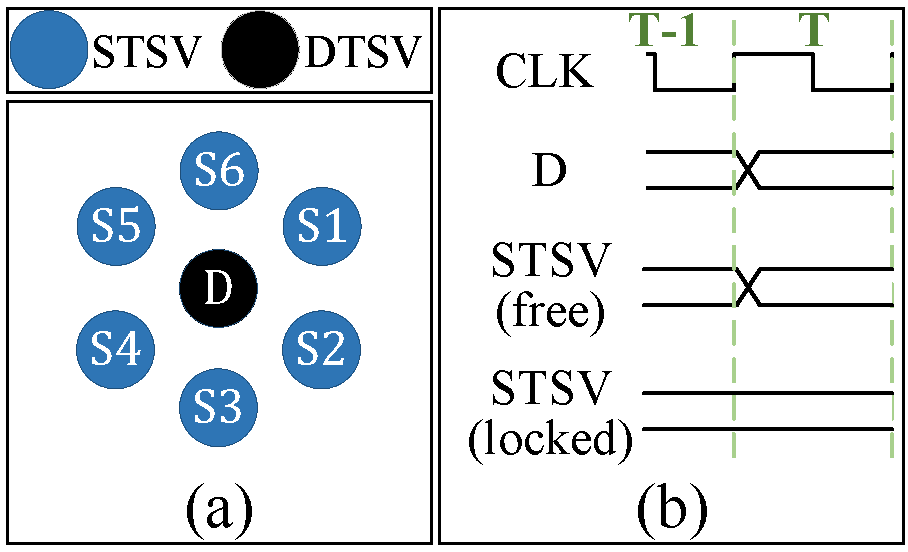
\includegraphics[width=1.6in]{./fig_files/BSCAC_oneGroup.pdf}
	\caption{A single encoding group in the BS-CAC scheme. (a) The layout of this group. (b) The timing diagram.}
	\label{fig-bscac_1group}
\end{figure}

(1) {\bf Free state}: It is permitted to transmit a logic value (i.e., 0 or 1) freely during this cycle, if an STSV is in the free state in cycle $T$.

(2) {\bf Locked state}: If an STSV is in the locked state in cycle $T$, its logic value remains the same as that in cycle $T-1$. 

For each STSV in the encoding group shown in Fig. \ref{fig-bscac_1group}, its state in cycle $T$ is determined by Algorithm \ref{alg-bscac}. Let the logic values transmitted on TSVs $\rm D$, $\rm S_1$, $\rm S_2$, $\rm S_3$, $\rm S_4$, $\rm S_5$  $\rm S_6$ at cycle $T-1$ be denoted as ${b'}_0,{b'}_1,{b'}_2,{b'}_3,{b'}_4,{b'}_5,{b'}_6$, respectively. Similarly, denote the logic alues transmitted on these TSVs at cycle  $T$ as $b_0,b_1,b_2,b_3,b_4,b_5,b_6$. The states of the six STSVs in cycle $T$ are discussed in the following two cases.

\begin{algorithm}
	\caption{The BS-CAC algorithm.}
	\label{alg-bscac}
	\DontPrintSemicolon
	\KwIn{The logic values ${b'}_0,{b'}_1,{b'}_2,{b'}_3,{b'}_4,{b'}_5,{b'}_6$ that are transmitted on the TSVs $\rm D$, $\rm S_1$, $\rm S_2$, $\rm S_3$, $\rm S_4$, $\rm S_5$, $\rm S_6$ at cycle $T-1$, respectively. The logic values $b_0,b_1,b_2,b_3,b_4,b_5,b_6$ that are waiting to be transmitted on the signal TSVs $\rm D$, $\rm S_1$, $\rm S_2$, $\rm S_3$, $\rm S_4$, $\rm S_5$, $\rm S_6$, respectively. }
	\KwOut{The set $\boldsymbol{F}$ which contains the signal TSVs with free state and the set $\boldsymbol{L}$ which contains the signal TSVs with locked state.}
	%	\Begin{
		$(\boldsymbol{F}, \boldsymbol{L}) = (\emptyset, \emptyset)$;\\
		\If{$b_0 = {b'}_0$}{
			$\boldsymbol{F} = \boldsymbol{F} + \{{\rm S_1}\}$;\\
			\For{$i=2$ {\rm to} $6$}{
				\If{${b'}_i = b_{i-1} \neq {b'}_{i-1}$ {\rm and} ${{\rm S}_{i-1}}\in \boldsymbol{F}$}{
					$\boldsymbol{L} = \boldsymbol{L} + \{{{\rm S}_i}\}$;}
			}
			\Else{
				$\boldsymbol{F} = \boldsymbol{F} + \{{{\rm S}_i}\}$;
			}
		}
		
		\Else{
			\If{${b'}_1 = {b'}_0$}{
				$\boldsymbol{F} = \boldsymbol{F} + \{{\rm S_1}\}$;
			}
			\ElseIf{${b'}_6 \neq {b'}_0$ {\rm and} ${b'}_2 \neq {b'}_0$}{
				$\boldsymbol{F} = \boldsymbol{F} + \{{\rm S_1}\}$;
			}
			\ElseIf{${b'}_6 = b_6 = {b'}_2 = b_2 = {b'}_0$}{
				$\boldsymbol{F} = \boldsymbol{F} + \{{\rm S_1}\}$;
			}
			\Else{
				$\boldsymbol{L} = \boldsymbol{L} + \{{\rm S_1}\}$;
			}
			
			\For{$i = 2$ {\rm to} $5$}{
				\If{${b'}_i = {b'}_0$}{
					$\boldsymbol{F} = \boldsymbol{F} + \{{\rm S}_i\}$;
				}
				\ElseIf{${b'}_{i-1} \neq {b'}_0$ {\rm and} ${b'}_{i+1} \neq {b'}_0$}{
					$\boldsymbol{F} = \boldsymbol{F} + \{{\rm S}_i\}$;
				}
				\ElseIf{${b'}_{i-1} \neq {b'}_0 = b_{i-1}$ {\rm and} ${\rm S}_{i-1}\in \boldsymbol{F}$}{
					$\boldsymbol{F} = \boldsymbol{F} + \{{\rm S}_i\}$;
				}
				\ElseIf{${b'}_{i-1} = b_{i-1} = {b'}_{i+1} = b_{i+1} = {b'}_0$}{
					$\boldsymbol{F} = \boldsymbol{F} + \{{\rm S}_i\}$;
				}
				\Else{
					$\boldsymbol{L} = \boldsymbol{L} + \{{\rm S}_i\}$;
				}
			}
			\If{${b'}_6 = {b'}_0$}{
				$\boldsymbol{F} = \boldsymbol{F} + \{{\rm S}_6\}$;
			}
			\ElseIf{${b'}_5 \neq {b'}_0$ {\rm and} ${b'}_1 \neq {b'}_0$}{
				$\boldsymbol{F} = \boldsymbol{F} + \{{\rm S}_6\}$;
			}
			\ElseIf{${b'}_5 \neq {b'}_0 = b_5$ {\rm and} ${\rm S}_5\in \boldsymbol{F}$}{
				$\boldsymbol{F} = \boldsymbol{F} + \{{\rm S}_6\}$;
			}
			\ElseIf{${b'}_1 \neq {b'}_0 = b_1$ {\rm and} ${\rm S}_1\in \boldsymbol{F}$}{
				$\boldsymbol{F} = \boldsymbol{F} + \{{\rm S}_6\}$;
			}
			\ElseIf{${b'}_5 = b_5 = {b'}_1 = b_1 = {b'}_0$}{
				$\boldsymbol{F} = \boldsymbol{F} + \{{\rm S}_6\}$;
			}
			\Else{
				$\boldsymbol{L} = \boldsymbol{L} + \{{\rm S}_6\}$;
			}
		}
		
		\Return{$\boldsymbol{F}, \boldsymbol{L}$\;}
	\end{algorithm}
	
{\bf Case 1:} Assume that the signal on the DTSV D has no transition in cycle $T$, i.e., $b_0={b'}_0$. In this case, the STSV $\rm S_1$ is always in the free state, and the STSV ${\rm S}_i$ ($i\in \{2,3,4,5,6\}$) is in the locked state only if the following two conditions are satisfied simultaneously.

Condition 1-1: The signal transmitted on ${\rm S}_{i-1}$ in cycle $T$ is different from that in cycle $T-1$ , i.e., ${\rm S}_i$ is in the free state in cycle $T$ and $b_{i-1}\neq {b'}_{i-1}$.

Condition 1-2: The signal transmitted on ${\rm S}_i$ is different from that transmitted on ${\rm S}_{i-1}$ in cycle $T-1$ , i.e., ${b'}_i\neq {b'}_{i-1}$.

{\bf Case 2:} Assume that the signal on the DTSV D has a transition in cycle $T$, i.e., $b_0\neq {b'}_0$. In this case, the STSV ${\rm S}_i$ ($i\in \{1,2,3,4,5,6\}$) is in the free state only if at least one of the following conditions is satisfied.

Condition 2-1: The signal transmitted on STSV ${\rm S}_i$ ($i\in \{1,2,3,4,5,6\}$) is the same as the signal transmitted on DTSV D in cycle $T-1$, i.e., ${b'}_i={b'}_0$.

Condition 2-2: The two STSVs that are in the same encoding group with ${\rm S}_i$ and directly adjacent to ${\rm S}_i$ do not satisfy the Condition 2-1. This condition is equivalent to ${b'}_{i-1} = {b'}_{i+1} \neq {b'}_0$ for $i\in \{2,3,4,5\}$. For $i=1$, this condition is equivalent to ${b'}_6 = {b'}_2 \neq {b'}_0$. For $i=6$, this condition is equivalent to ${b'}_5 = {b'}_1 \neq {b'}_0$.

Condition 2-3: The two STSVs that are in the same encoding group with ${\rm S}_i$ and directly adjacent to ${\rm S}_i$ satisfy Condition 2-1, and the signals transmitted on them in cycle $T$ have no transition. This condition is equivalent to ${b'}_{i-1} = {b'}_{i+1} = {b'}_0 = b_{i-1} = b_{i+1}$ for $i\in \{2,3,4,5\}$. For $i=1$, this condition is equivalent to  ${b'}_6 = {b'}_2 = {b'}_0 = b_6 = b_2$. For $i=6$, this condition is equivalent to ${b'}_5 = {b'}_1 = {b'}_0 = b_5 = b_1$.

Condition 2-4 (for ${\rm S}_2\sim {\rm S}_6$ only): The STSV ${\rm S}_{i-1}$ ($i\in \{ 2,3,4,5,6\}$) does not satisfy Condition 2-1 and the signal transmitted on it has a transition in cycle $T$, i.e., ${b'}_{i-1} \neq {b'}_0 = b_{i-1}$ and ${\rm S}_{i-1}$ is in the free state in cycle $T$.

Condition 2-5 (for ${\rm S}_6$ only): The signal ${\rm S}_1$ does not satisfy Condition 2-1 and the signal transmitted on it has a transition in cycle $T$, i.e., ${b'}_1 \neq {b'}_0 = b_1$ and ${\rm S}_1$ is in the free state in cycle $T$.

\subsection{The encoding process with the optimal 2C-reduction dynamic shielding layout in hexagonal arrays}\label{subsec-bscac-process}
As defined in Part \ref{subsec-dysh-intro}, an encoding group consists of one DTSV that is in the non-shielding state and six STSVs surrounding this DTSV. In the dynamic shielding scheme proposed in Part \ref{subsec-dysh-layout}, each STSV is directly adjacent to one DTSV of type D1, one DTSV of type D2, and one DTSV of type D3 on the premise of disregarding the boundary of the array. The non-shielding cycles of these three types of DTSVs encompass all the transmission cycles and do not overlap with each other. Therefore, for each STSV, there is exactly one DTSV that is in the non-shielding state and is directly adjacent to it. This indicates that any one STSV in Fig. \ref{fig-dysh_layout} can be categorized into exactly one encoding group in each transmission cycle on the premise of disregarding the boundary of the array. For example, Fig. \ref{fig-bscac_3groups}(a) shows a part of the layout proposed in Part \ref{subsec-dysh-layout}, in which the STSV A are encoded in one of the following three encoding groups:

\begin{figure}[t]
	\centering
	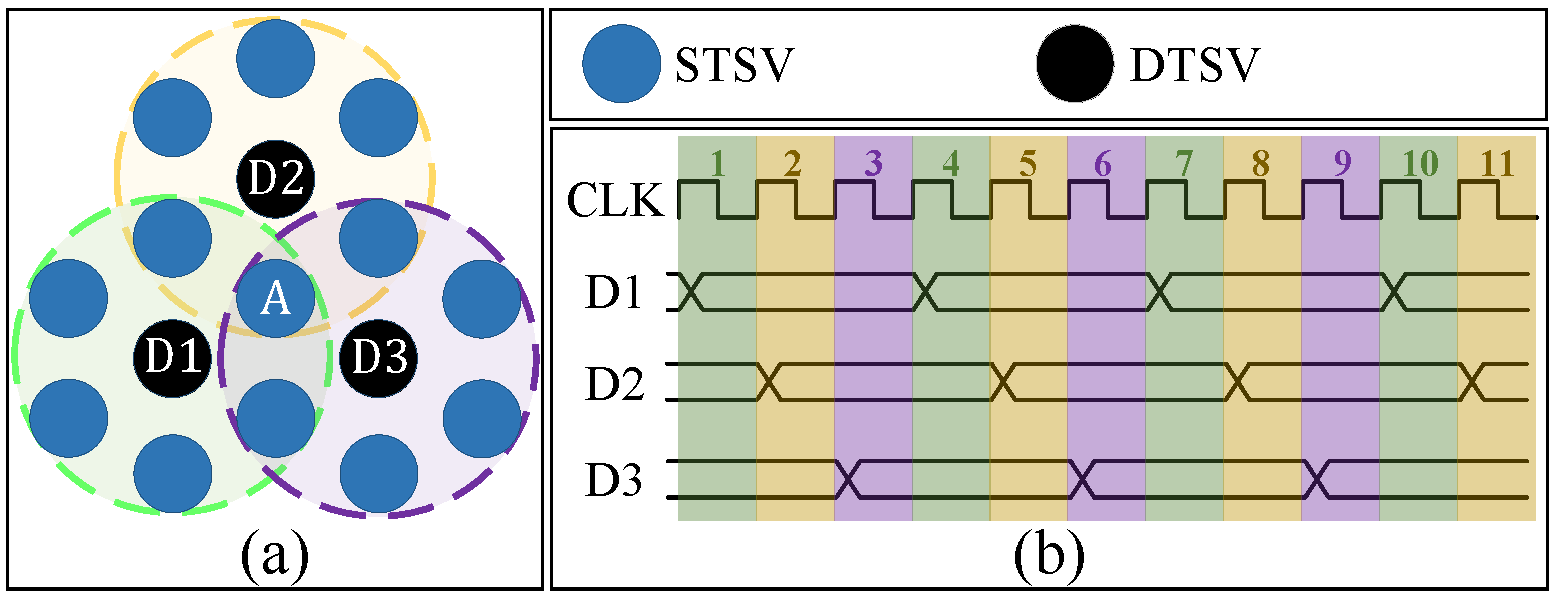
\includegraphics[width=2.7in]{./fig_files/BSCAC_3Groups.pdf}
	\caption{A part of the layout proposed in Part III-B. (a) The STSV A and its three encoding group. (b) The timing diagram.}
	\label{fig-bscac_3groups}
\end{figure}

(1) The transmission cycles marked in green in Fig. \ref{fig-bscac_3groups}(b) are the non-shielding cycles of D1-type DTSVs. In these cycles, the STSV A are categorized into an encoding group centered on a D1-type DTSV, and this encoding group is surrounded by the green dashed line in Fig. \ref{fig-bscac_3groups}(a).

(2) The transmission cycles marked in yellow in Fig. \ref{fig-bscac_3groups}(b) are the non-shielding cycles of D2-type DTSVs. In these cycles, the STSV A are categorized into an encoding group centered on a D2-type DTSV, and this encoding group is surrounded by the yellow dashed line in Fig. \ref{fig-bscac_3groups}(a).

(3) The transmission cycles marked in purple in Fig. \ref{fig-bscac_3groups}(b) are the non-shielding cycles of D3-type DTSVs. In these cycles, the STSV A are categorized into an encoding group centered on a D3-type DTSV, and this encoding group is surrounded by the purple dashed line in Fig. \ref{fig-bscac_3groups}(a).

The above discussions assume that the array is unbounded. However, the TSV arrays have boundaries in practice, and some TSVs located near the boundaries may not be categorized into a complete encoding group in some transmission cycles. The encoding rules for this case are as follows:

{\bf Case 1:} An STSV is directly adjacent to a DTSV that is in the non-shielding state in the current cycle, but the encoding group centered on this DTSV is incomplete. This incomplete encoding group is processed according to Algorithm \ref{alg-bscac}, in which all the input variables related to the non-existent STSVs are assigned to 0. Fig. \ref{fig-bscac_edgeTSVs}(a) shows an example, in which the STSV A is categorized into the incomplete encoding group surrounded by the red line. As shown in Fig. \ref{fig-bscac_edgeTSVs}(b), the states of the STSVs in this group are determined by Algorithm \ref{alg-bscac}, and the data transmitted on the non-existent STSVs (marked in yellow) are regarded as 0.

%{\bf Case 1:} An STSV is directly adjacent to a DTSV that is in the non-shielding state in the current cycle, while the encoding group centered on this DTSV is incomplete. In this case, the incomplete group is processed according to Algorithm \ref{alg-bscac}, where all input variables corresponding to the non-existent STSVs are assigned a value of 0.
%Fig. \ref{fig-bscac_edgeTSVs}(a) illustrates an example in which STSV A belongs to an incomplete encoding group outlined in red. As shown in Fig. \ref{fig-bscac_edgeTSVs}(b), the states of the STSVs in this group are determined by Algorithm \ref{alg-bscac}, and the data transmitted on the non-existent STSVs (highlighted in yellow) are treated as 0.

{\bf Case 2:} All the directly adjacent DTSVs of the STSV are not in the non-shielding state in the current cycle. The STSV A in Fig. \ref{fig-bscac_edgeTSVs}(c) is an instance which conforms to this case. As shown in Fig. \ref{fig-bscac_edgeTSVs}(d), the encoding group containing the STSV A is centered around a virtual DTSV (marked in green in Fig. \ref{fig-bscac_edgeTSVs}(d)) that actually does not exist. Then this encoding group is processed according to the rules in Case 1, and the signals transmitted on the virtual DTSV are always regarded as 0.

\begin{figure}[t]
	\centering
	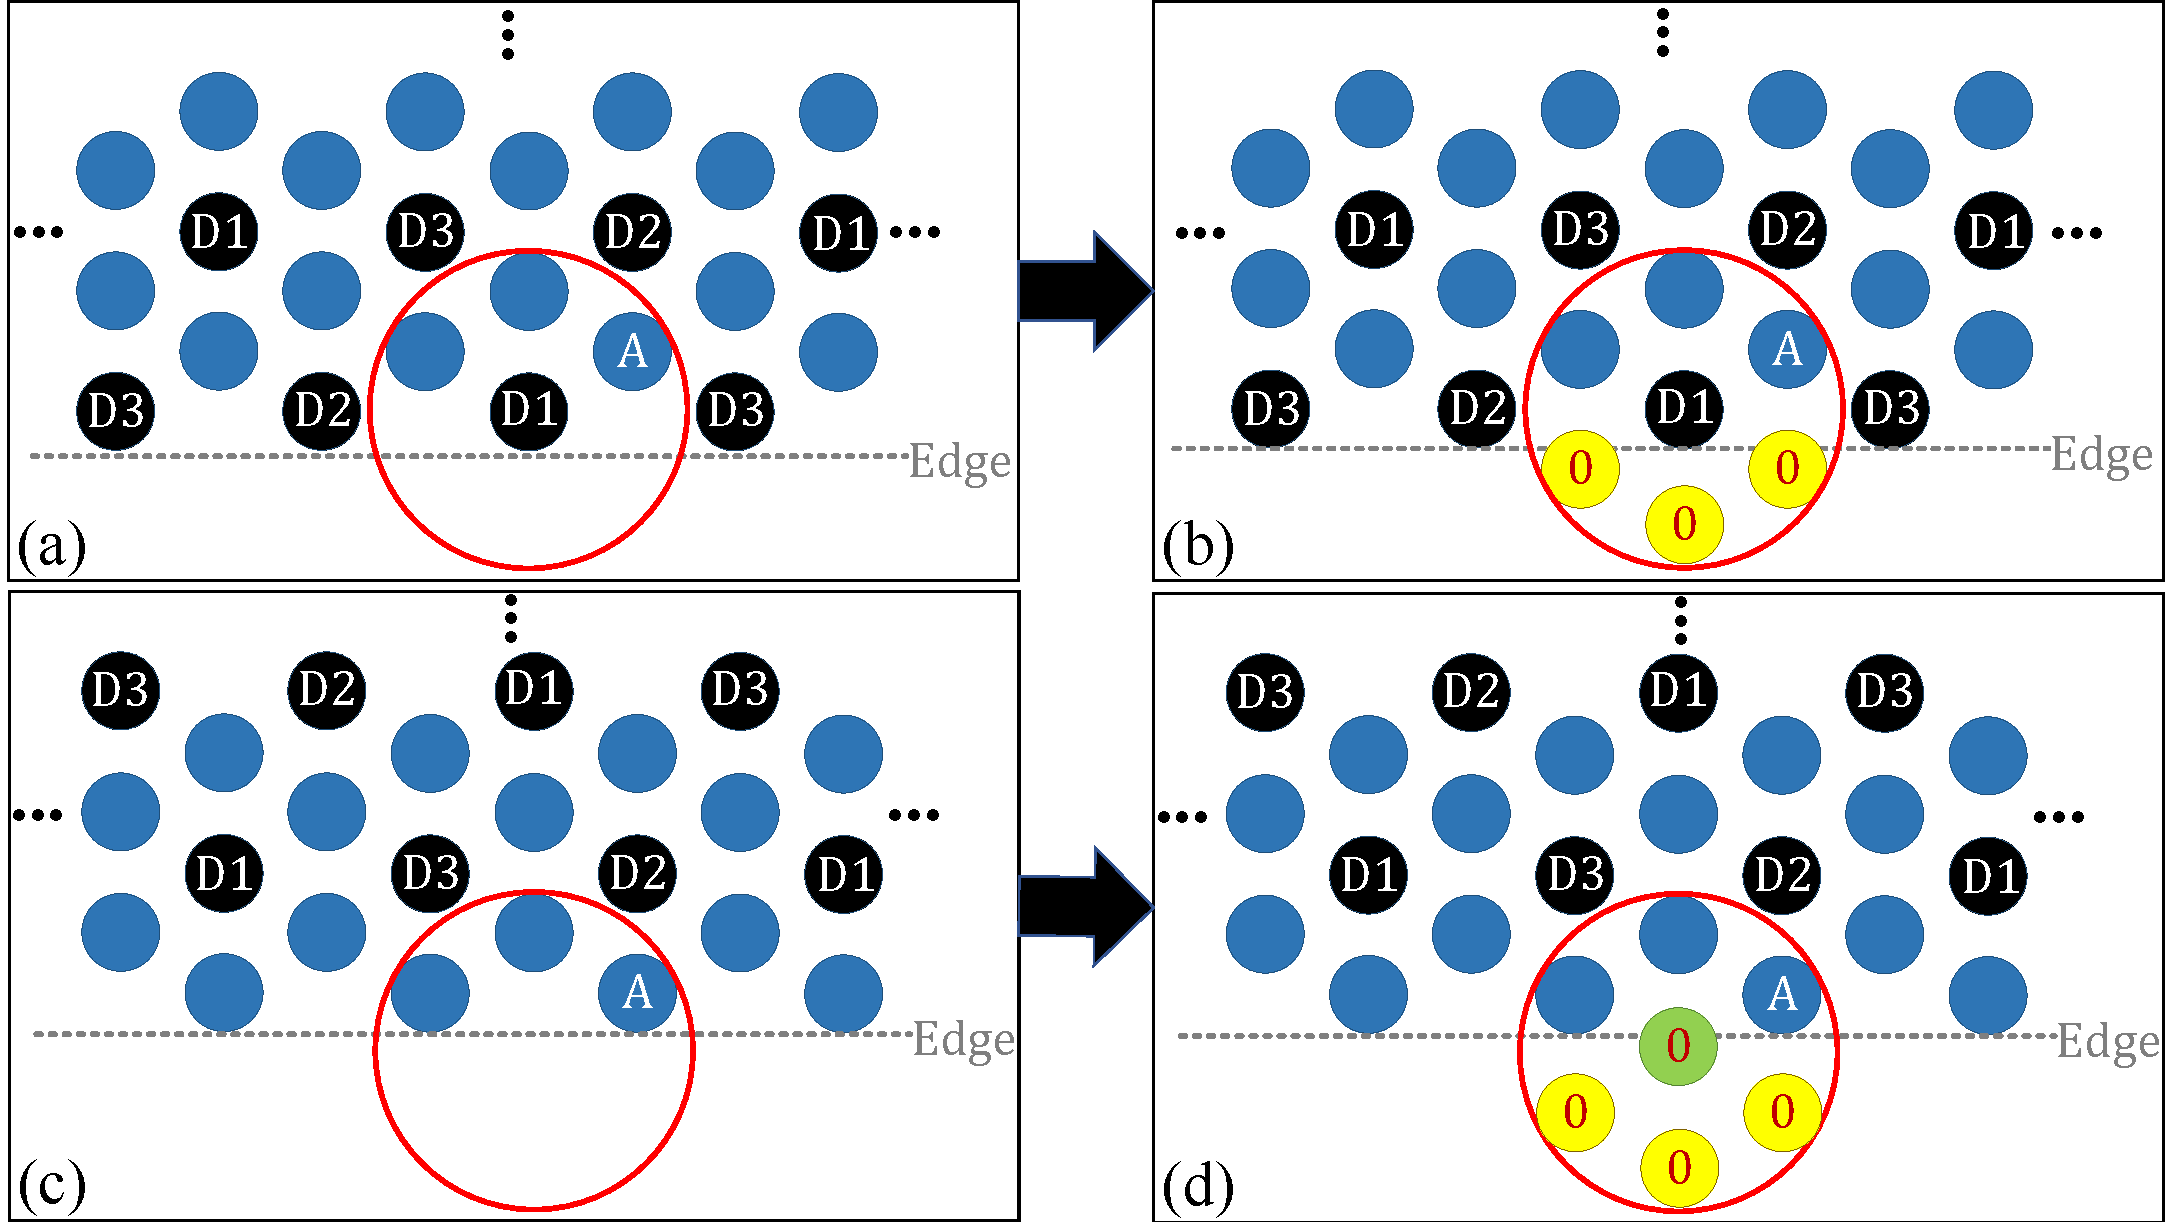
\includegraphics[width=3.2in]{./fig_files/dysh_edgeTSVs.pdf}
	\caption{The encoding rules for the incomplete encoding groups. The incomplete encoding group in (a) is encoded by regarding the data transmitted on the non-existent STSVs (marked in yellow) as 0, as shown in (b); The incomplete encoding group in (c) is encoded by assigning the data transmitted on the non-existent DTSV (marked in green) and STSVs (marked in yellow) to 0, as shown in (d).}
	\label{fig-bscac_edgeTSVs}
\end{figure}

The virtual TSVs used for completing the encoding group, which are marked in yellow or green in Fig. \ref{fig-bscac_edgeTSVs}, do not actually exist. Therefore, some logic modules can be eliminated to reduce the hardware overhead when implementing the codecs for the groups with virtual TSVs.

\section{The code efficiency}\label{sec-code_rate}
\subsection{The theoretical code efficiency}\label{subsec-code_rate-calc}
The code efficiency is defined as the average number of effective data bits transmitted by each TSV during each cycle in a TSV array. In the hexagonal TSV arrays adopting the proposed BS-CAC scheme, the theoretical code efficiency is always less than 1, because the STSVs in the locked state and the DTSVs in the shielding state cannot transmit any effective data bit. The analysis of the code efficiency is of paramount importance for the application of the proposed scheme, as it offers the designers an estimation of the data transmission rate of the whole array during the normal operation process. This Part discusses the computation method of the coding efficiency of the BS-CAC scheme.

For the arrays applying the proposed BS-CAC scheme, the minimum time required for the data bits on all TSVs to flip is referred to as one period. In this paper, the term \textbf{period} refers to three consecutive transmission cycles, because the DTSVs of three different types consume at least three consecutive cycles to undergo one non-shielding cycle respectively. Define the data bits transmitted on the TSV array as the array state. The array state is a stochastic process $\{\boldsymbol{X}(t)\}$ if one period is regarded as the time unit. The sequence $\boldsymbol{X}(t)$ represents the array state after $t$ periods from the initial array state. Denote the state space of $\{\boldsymbol{X}(t)\}$ (i.e., the set of states that $\{\boldsymbol{X}(t)\}$ can take) as $\boldsymbol{S}$. According to Section \ref{sec-dysh} and \ref{sec-bscac}, the following formulas hold, where the symbol $\rm Pr()$ represents probability.

\begin{equation}
	\begin{aligned}
		{\rm Pr}( \boldsymbol{X}(t+1) = &x_{t+1} | \\
		&\boldsymbol{X}(t)=x_t, \boldsymbol{X}(t-1)=x_{t-1}, ...,\boldsymbol{X}(1)=x_1 ) \\
		={\rm Pr}( \boldsymbol{X}(t+1) &= x_{t+1} | \boldsymbol{X}(t)=x_t ), x_i \in \boldsymbol{S}
	\end{aligned}
	\label{eq-5.2.1}
\end{equation}

\begin{equation}
	\begin{aligned}
		{\rm Pr}( \boldsymbol{X}(t+1) = x_{\rm b}& | \boldsymbol{X}(t) = x_{\rm a})\\
		={\rm Pr}&( \boldsymbol{X}(2) = x_{\rm b} | \boldsymbol{X}(1) = x_{\rm a}),
		x_{\rm a} \in \boldsymbol{S}, x_{\rm b} \in \boldsymbol{S}
	\end{aligned}
	\label{eq-5.2.2}
\end{equation}


According to formulas (\ref{eq-5.2.1}) and  (\ref{eq-5.2.2}), the stochastic process $\{\boldsymbol{X}(t)\}$ is a time-invariant discrete-time Markov chain.

\begin{theorem}\label{theorem-5.2.4}
	For Markov chain $\{\boldsymbol{X}(t)\}$, there exists a unique stationary distribution $\boldsymbol{\mu}$. The distribution of $\{\boldsymbol{X}(t)\}$ tends to this unique stationary distribution $\boldsymbol{\mu}$ as $t\to \infty$.
\end{theorem}

The proof process of Theorem \ref{theorem-5.2.4} is given in Appendix. Denote the unique stationary distribution of $\{\boldsymbol{X}(t)\}$ as $\boldsymbol{\mu}$. The elements of $\boldsymbol{\mu}$ are the probability value of each state. The formula (\ref{eq-5.2.4}) holds.

\begin{equation}
	\begin{aligned}
		\left\{ 
		\begin{matrix}
			\boldsymbol{\mu P} = \boldsymbol{\mu} \\
			\sum\limits_{i} \boldsymbol{\mu}[i] = 1
			\label{eq-5.2.4}
		\end{matrix}
		\right.
	\end{aligned}
\end{equation}

\noindent in which the symbol $\boldsymbol{P}$ is the probability transition matrix. The element $\boldsymbol{P}[i,j]$ is the probability of state $x_i$ transiting to $x_j$ after one period. In the probability transition matrix $\boldsymbol{P}$, the number of rows and the number of columns are equal to the size of state space $\boldsymbol{S}$, which is denoted as ${\rm card}(\boldsymbol{S})$. And the sum of the elements in each row and the sum of the elements in each column of $\boldsymbol{P}$ are 1. The probability transition matrix $\boldsymbol{P}$ can be calculated by the exhaustive algorithm presented in Algorithm \ref{alg-5.1.1}. Denote the number of the TSVs in the array as $N_{\rm TSV}$. In Algorithm \ref{alg-5.1.1}, the symbol $r_j^3\in \boldsymbol{R}^3 $ is the three-cycle data waiting to be transmitted in the next period. It contains $3N_{\rm TSV}$ binary elements, i.e., the first three data bits in the transmission queue of each TSV. The symbol $\boldsymbol{R}^3=\{r_1^3,r_2^3,...\}$ is the set of the three-cycle data waiting to be transmitted in the next period, and the symbol ${\rm Pr}(r_i^3)$ is the distribution probability of the element $r_i^3$ in set $\boldsymbol{R}^3$. The $\boldsymbol{R}^3$ and ${\rm Pr}(r_i^3)$ are related to the pattern of the data bits to be transmitted. For example, if the data bits to be transmitted are independent of each other and conform to the Bernoulli distribution in which bit 0 and bit 1 share the same probability, the set $\boldsymbol{R}^3$ contains $2^{3N_{\rm TSV}}$ elements, and the distribution probability ${\rm Pr}(r_i^3)$ of each element is $1/2^{3N_{\rm TSV}}$. For a given $r_j^3$ and a given array state $x_i$, the array state after one period changes to $x'={\rm BSEnc3}(x_i,r_j^3)$, in which the $x'={\rm BSEnc3}(x_i,r_j^3)$ is obtained uniquely according to the algorithms in Section \ref{sec-dysh} and Section \ref{sec-bscac}.

\begin{algorithm}
	\caption{Computation of the probability transition matrix $\boldsymbol{P}$.}
	\label{alg-5.1.1}
	\DontPrintSemicolon
	\KwIn{The set of the three-cycle data waiting to be transmitted in the next period is $\boldsymbol{R}^3=\{r_1^3,r_2^3,...\}$. The distribution probability of $r_i^3$ is ${\rm Pr}(r_i^3)$. The state space of $\{\boldsymbol{X}(t)\}$ is $\boldsymbol{S}$.}
	\KwOut{The probability transition matrix $\boldsymbol{P}$.}
	%	\Begin{
		$\boldsymbol{P} = \boldsymbol{0}_{{\rm card}(\boldsymbol{S})\times {\rm card}(\boldsymbol{S})}$;\\
		\ForEach{$x_i \in \boldsymbol{S}$}{
			\ForEach{$r_j^3\in \boldsymbol{R}^3$}{
				$x' = {\rm BSEnc3}(x_i, r_j^3)$;\\
				$\boldsymbol{P}[x_i,x'] = \boldsymbol{P}[x_i,x']+{\rm Pr}(r_j^3)$;
			}
		}
				
	\Return{$\boldsymbol{P}$;}
\end{algorithm}

The stationary distribution $\boldsymbol{\mu}$ can be calculated from formula (\ref{eq-5.2.4}) after the probability transition matrix $\boldsymbol{P}$ is obtained. The expectation ${\rm E}(n_{\rm trans})$ of the number of effective data bits transmitted during each period can be calculated by the following formula (\ref{eq-5.2.5}).

\begin{equation}
	{\rm E}(n_{\rm trans}) = \sum_{i\in [0, {\rm card}(\boldsymbol{S})]}^{} (\boldsymbol{\mu}[i] \sum_{r_j^3 \in \boldsymbol{R}^3}^{} D(x_i,r_j^3) {\rm Pr}(r_j^3))
	\label{eq-5.2.5}
\end{equation}

\noindent where the symbol $D(x_i,r_j^3)$ represents the number of effective data bits transmitted (i.e., the sum of the number of STSVs marked as the free state in each cycle and the number of DTSVs in the array) during a period when the last state before this period is $x_i$ and the data waiting to be transmitted is $r_j^3$.

The procedure offered in this part is able to compute the theoretical expectation of the number of effective data bits transmitted through a hexagonal array with the proposed BS-CAC scheme accurately. However, this is not practical for large-scale arrays. The reason is that as the array size increases, the time required to compute the probability transition matrix $\boldsymbol{P}$ and the stationary distribution $\boldsymbol{\mu}$ becomes increasingly unacceptable. In order to evaluate the code efficiency of the proposed scheme in the large-scale arrays, the simplified computation process is required based on some assumptions in the following parts. 

\subsection{The estimation of the theoretical code efficiency in the borderless array}\label{subsec-code_rate-esti_borderless}
All the discussions in this part are based on the following assumptions.
(1) The array is assumed to be infinite, i.e., the boundaries of the array are ignored.
(2) The data bits to be transmitted are assumed to be independent of each other and conform to the Bernoulli distribution in which bit 0 and bit 1 share the same probability.

As shown in Fig. \ref{fig-bscac_1group}, the transmission cycles can be divided into the following three categories in the proposed scheme: the non-shielding cycles of type-D1, type-D2 and type-D3 DTSVs (marked in green, yellow and purple in Fig. \ref{fig-bscac_1group}(b)), respectively. The Markov chain $\{\boldsymbol{X}(t)\}$ is defined by taking one period as the minimum time unit, and its initial state is not constrained to any particular transmission cycle. Therefore, there are three Markov chains existing simultaneously in an array:

(1) $\{\boldsymbol{X}_{\rm D1}(t)\}$: The initial state of $\{\boldsymbol{X}_{\rm D1}(t)\}$ is in a non-shielding cycle of the type-D1 DTSVs. Since one period contains three consecutive transmission cycles, all the subsequent states of $\{\boldsymbol{X}_{\rm D1}(t)\}$ are in the non-shielding cycles of type-D1 DTSVs. The state space and stationary distribution of $\{\boldsymbol{X}_{\rm D1}(t)\}$ are denoted as $\boldsymbol{S}^{\rm D1}$ and $\boldsymbol{\mu}^{\rm D1}$, respectively.

(2) $\{\boldsymbol{X}_{\rm D2}(t)\}$: The initial state and the subsequent states of $\{\boldsymbol{X}_{\rm D2}(t)\}$ are in the non-shielding cycles of type-D2 DTSVs. The state space and stationary distribution of $\{\boldsymbol{X}_{\rm D2}(t)\}$ are denoted as $\boldsymbol{S}^{\rm D2}$ and $\boldsymbol{\mu}^{\rm D2}$, respectively.

(3) $\{\boldsymbol{X}_{\rm D3}(t)\}$: The initial state and the subsequent states of $\{\boldsymbol{X}_{\rm D3}(t)\}$ are in the non-shielding cycles of type-D3 DTSVs. The state space and stationary distribution of $\{\boldsymbol{X}_{\rm D3}(t)\}$ are denoted as $\boldsymbol{S}^{\rm D3}$ and $\boldsymbol{\mu}^{\rm D3}$, respectively.

The discussions in Part \ref{subsec-code_rate-calc} are applicable to $\{\boldsymbol{X}_{\rm D1}(t)\}$, $\{\boldsymbol{X}_{\rm D2}(t)\}$ and $\{\boldsymbol{X}_{\rm D3}(t)\}$. In the non-shielding cycles of type-D1 DTSVs, each STSV is categorized into an encoding group centered around a type-D1 DTSV. Fig. \ref{fig-5.2.1}(a) shows an example, where GP1 and GP2 are two encoding groups centered around the type-D1 DTSV. When  $\{\boldsymbol{X}_{\rm D1}(t)\}$ tends to this stationary distribution, the distribution of the state of all STSVs (abbreviated as the STSVs state) in GP1 and GP2 tend to $\boldsymbol{\mu}^{\rm GP1}$ and $\boldsymbol{\mu}^{\rm GP2}$. The distributions $\boldsymbol{\mu}^{\rm GP1}$ and $\boldsymbol{\mu}^{\rm GP2}$ are unique because the stationary distribution of $\{\boldsymbol{X}_{\rm D1}(t)\}$ is unique. And the $\boldsymbol{\mu}^{\rm GP1}$ and $\boldsymbol{\mu}^{\rm GP2}$ can be calculated by the following formula (\ref{eq-5.2.5x}).

\begin{equation}
	\begin{aligned}
		\left\{ 
		\begin{matrix}
			\boldsymbol{\mu}^{\rm GP1}[x_i^{\rm GP1}] = \sum\limits_{\forall x_j \to x_i^{\rm GP1}}^{} \boldsymbol{\mu}^{\rm D1}[x_j] \\
			\boldsymbol{\mu}^{\rm GP2}[x_i^{\rm GP2}] = \sum\limits_{\forall x_j \to x_i^{\rm GP2}}^{} \boldsymbol{\mu}^{\rm D1}[x_j]
			\label{eq-5.2.5x}
		\end{matrix}
		\right.
	\end{aligned}
\end{equation}

\begin{figure}[t]
	\centering
	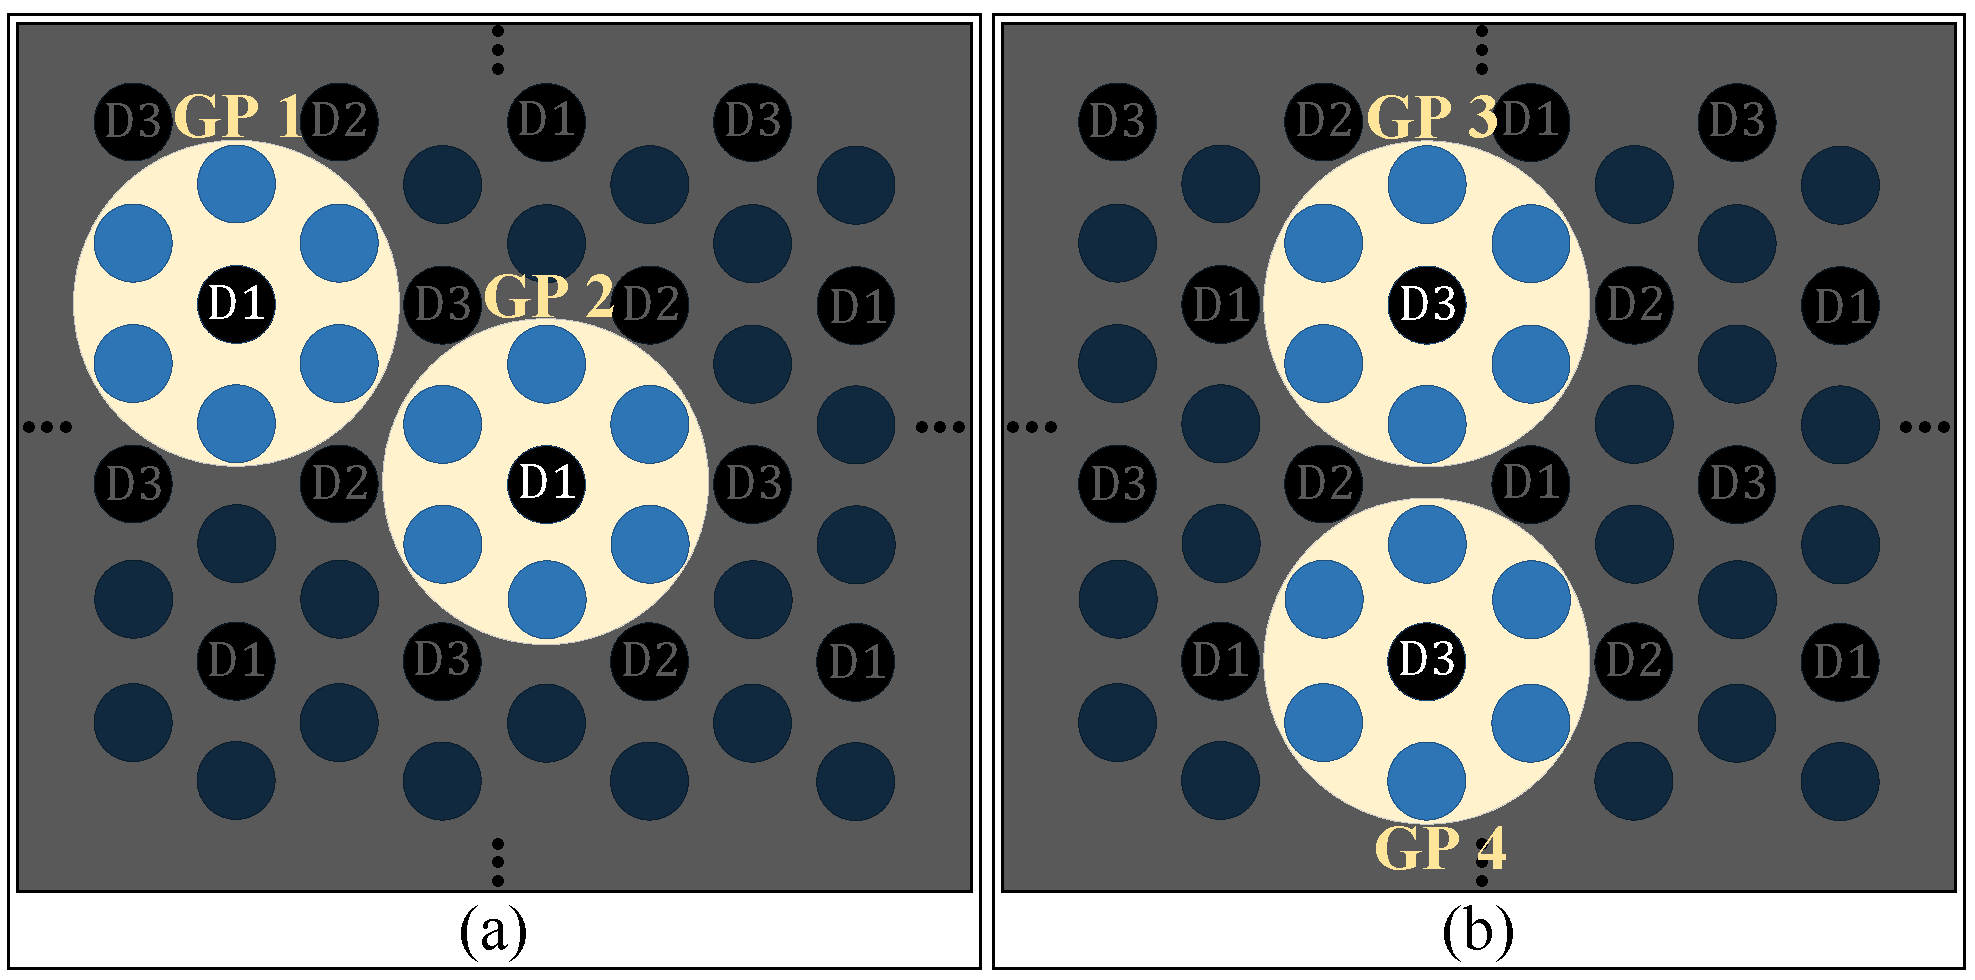
\includegraphics[width=3.0in]{./fig_files/fig_5.2.1.pdf}
	\caption{Four encoding groups. The GP1 and GP2 in (a) are two encoding groups centered around the type-D1 DTSV. The GP3 and GP4 in (b) are two encoding groups centered around the type-D3 DTSV.}
	\label{fig-5.2.1}
\end{figure}

\noindent in which $x_i^{\rm GP1}\in \boldsymbol{S}^{\rm GP1}$ and $x_i^{\rm GP2}\in \boldsymbol{S}^{\rm GP2}$ are the STSVs state in GP1 and GP2, respectively, and $\boldsymbol{S}^{\rm GP1}$ and $\boldsymbol{S}^{\rm GP2}$ are the state spaces. The operator $\to$ represents the logic implication. For example, the expression $x_j\to x_i^{\rm GP1}$ represents that the STSVs state in GP1 is $x_i^{\rm GP1}\in \boldsymbol{S}^{\rm GP1}$ when the array state is $x_j\in \boldsymbol{S}^{\rm D1}$.
 
Denote the probability transition matrices of GP1 and GP2 as $\boldsymbol{P}^{\rm GP1}$ and $\boldsymbol{P}^{\rm GP2}$, respectively. The element $\boldsymbol{P}^{\rm GP1}[i,j]$ is the probability of state $x_i^{\rm GP1}\in \boldsymbol{S}^{\rm GP1}$ transiting to $x_j^{\rm GP1}\in \boldsymbol{S}^{\rm GP1}$ after one period, and the element $\boldsymbol{P}^{\rm GP2}[i,j]$ is the probability of state  $x_i^{\rm GP2}\in \boldsymbol{S}^{\rm GP2}$ transiting to $x_j^{\rm GP2}\in \boldsymbol{S}^{\rm GP2}$ after one period. The formula (\ref{eq-5.2.6}) holds because the distribution $\boldsymbol{\mu}^{\rm GP1}$ and $\boldsymbol{\mu}^{\rm GP2}$ are derived from the stationary distribution of $\{\boldsymbol{X}_{\rm D1}(t)\}$.

\begin{equation}
	\begin{aligned}
		\left\{ 
		\begin{matrix}
			\boldsymbol{\mu}^{\rm GP1} \boldsymbol{P}^{\rm GP1} = \boldsymbol{\mu}^{\rm GP1}, \
			\boldsymbol{\mu}^{\rm GP2} \boldsymbol{P}^{\rm GP2} = \boldsymbol{\mu}^{\rm GP2} \\
			\sum\limits_{i} \boldsymbol{\mu}^{\rm GP1}[i] = \sum\limits_{i} \boldsymbol{\mu}^{\rm GP2}[i] = 1
			\label{eq-5.2.6}
		\end{matrix}
		\right.
	\end{aligned}
\end{equation}

Similarly, in the non-shielding cycles of type-D3 DTSVs, each STSV is categorized into an encoding group centered around a type-D3 DTSV. Fig. \ref{fig-5.2.1}(b) shows an example, in which GP3 and GP4 are two encoding groups centered around the type-D3 DTSV. When $\{\boldsymbol{X}_{\rm D3}(t)\}$ tends to this stationary distribution, the distribution of the state of all STSVs (abbreviated as the STSVs state) in GP3 and GP4 tend to $\boldsymbol{\mu}^{\rm GP3}$ and $\boldsymbol{\mu}^{\rm GP4}$, respectively. And the formula (\ref{eq-5.2.7}) holds. 

\begin{equation}
	\begin{aligned}
		\left\{ 
		\begin{matrix}
			\boldsymbol{\mu}^{\rm GP3} \boldsymbol{P}^{\rm GP3} = \boldsymbol{\mu}^{\rm GP3},\
			\boldsymbol{\mu}^{\rm GP4} \boldsymbol{P}^{\rm GP4} = \boldsymbol{\mu}^{\rm GP4} \\
			\sum\limits_{i} \boldsymbol{\mu}^{\rm GP3}[i] = \sum\limits_{i} \boldsymbol{\mu}^{\rm GP4}[i] = 1
			\label{eq-5.2.7}
		\end{matrix}
		\right.
	\end{aligned}
\end{equation}



It can be deduced from the two assumptions in this part that $\boldsymbol{P}^{\rm GP1} = \boldsymbol{P}^{\rm GP2} = \boldsymbol{P}^{\rm GP3} = \boldsymbol{P}^{\rm GP4}$. Therefore, $\boldsymbol{\mu}^{\rm GP1} = \boldsymbol{\mu}^{\rm GP2} = \boldsymbol{\mu}^{\rm GP3} = \boldsymbol{\mu}^{\rm GP4}$. Consider the sub-array shown in Fig. \ref{fig-5.2.2}, in which GP5 is an encoding group centered around a type-D1 DTSV and GP6$\sim$GP8 are three encoding groups centered around a type-D3 DTSV. When $\{\boldsymbol{X}_{\rm D1}(t)\}$ and $\{\boldsymbol{X}_{\rm D3}(t)\}$ tend to the unique stationary distribution, the distributions in GP5$\sim$GP8 tend to $\boldsymbol{\mu}^{\rm GP5}$, $\boldsymbol{\mu}^{\rm GP6}$, $\boldsymbol{\mu}^{\rm GP7}$, and $\boldsymbol{\mu}^{\rm GP8}$, respectively. According to the above discussions, the formula (\ref{eq-5.2.8}) holds. 

\begin{equation}
	\boldsymbol{\mu}^{\rm GP5} = \boldsymbol{\mu}^{\rm GP6} = \boldsymbol{\mu}^{\rm GP7} = \boldsymbol{\mu}^{\rm GP8}
	\label{eq-5.2.8}
\end{equation}

\begin{figure}[t]
	\centering
	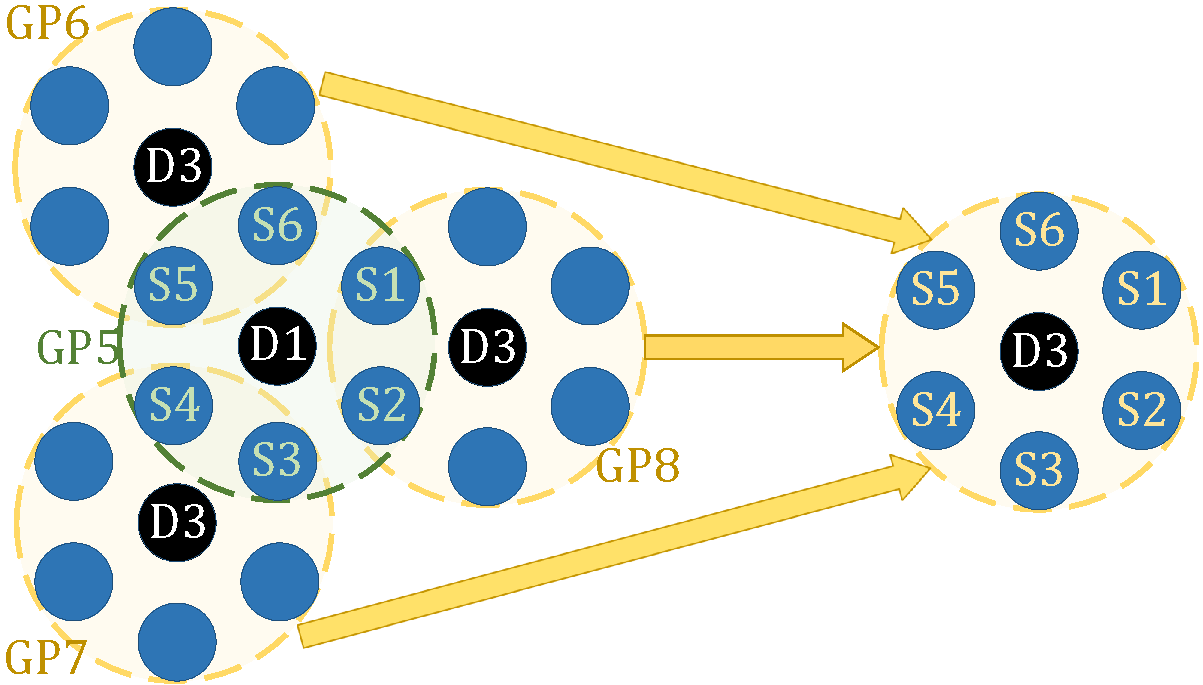
\includegraphics[width=2.0in]{./fig_files/fig_5.2.2.pdf}
	\caption{Correspondence between the STSVs in D1-type and D3-type encoding groups, in which GP5 is a D1-type encoding group and GP6$\sim$GP8 are three D3-type groups.}
	\label{fig-5.2.2}
\end{figure}

Denote the transition probability transition matrix of the STSVs S1$\sim$S6 from cycle $T$ to cycle $T+1$ as $\boldsymbol{Q}_{\rm D3\to D1}^{\rm GP5}$. The formulas (\ref{eq-5.2.9}) and (\ref{eq-5.2.10}) hold, in which the bit indexes of the variables $x_j^{\rm GP5}$, $x_j^{\rm GP6}$, $x_j^{\rm GP7}$ and $x_j^{\rm GP8}$ start from 1 rather than 0 for the convenience of reading. For example, the symbol $x_j^{\rm GP5}[1]$ represents the logic value on the STSV S1 in Fig. \ref{fig-5.2.2}.

\begin{equation}
	\begin{aligned}
		&\boldsymbol{\mu}^{\rm GP5, cycleT}[i] \\
		&=( \sum_{\forall (x_j^{\rm GP6}[3],x_j^{\rm GP6}[2]) = (x_i^{\rm GP5}[5],x_j^{\rm GP5}[6])}^{} \boldsymbol{\mu}^{\rm GP6}[j] ) \\	
		&\times ( \sum_{\forall (x_j^{\rm GP7}[1],x_j^{\rm GP7}[6]) = (x_i^{\rm GP5}[3],x_j^{\rm GP5}[4])}^{} \boldsymbol{\mu}^{\rm GP7}[j] ) \\	
		&\times ( \sum_{\forall (x_j^{\rm GP8}[5],x_j^{\rm GP8}[4]) = (x_i^{\rm GP5}[1],x_j^{\rm GP5}[2])}^{} \boldsymbol{\mu}^{\rm GP8}[j] ) \\		
	\end{aligned}
	\label{eq-5.2.9}
\end{equation}

%\begin{equation}
%	\begin{aligned}
%		\left\{ 
%		\begin{matrix}
%			\boldsymbol{\mu}^{\rm GP5} = \boldsymbol{\mu}^{\rm GP5, cycleT}\boldsymbol{Q}_{\rm D3\to D1}^{\rm GP5} \\
%			\sum\limits_{i}^{} \boldsymbol{\mu}^{\rm GP5}[i]=1
%			\label{eq-5.2.10}
%		\end{matrix}
%		\right.
%	\end{aligned}
%\end{equation}

\begin{equation}
	\left\{
	\begin{aligned}
		\boldsymbol{\mu}^{\rm GP5} &= \boldsymbol{\mu}^{\rm GP5,cycleT}\boldsymbol{Q}_{\rm D3\to D1}^{\rm GP5},\\
		\sum_i \boldsymbol{\mu}^{\rm GP5}[i] &= 1
	\end{aligned}
	\right.
	\label{eq-5.2.10}
\end{equation}

$\boldsymbol{Q}_{\rm D3\to D1}^{\rm GP5}$ can be obtained by Algorithm \ref{alg-5.2.1}, in which the ${\rm BSEnc1}(x_i,r_j)$ represents the state of STSVs S1$\to$S6 in cycle $T+1$ in the case that the state of STSVs S1$\to$S6 in cycle $T$ is $x_i$ and the six-bit data (one bit for each STSV) in the transmission queue is $r_j$. The $\boldsymbol{\mu}^{\rm GP5, cycleT}$ can be calculated according to the Algorithm \ref{alg-5.2.1} and the above formulas (\ref{eq-5.2.8})$\sim$(\ref{eq-5.2.10}). The expected width ${\rm E}(n_{\rm trans,STSV})$ of the effective data bits transmitted by the STSVs of GP5 in cycle $T+1$ can be obtained from formula (\ref{eq-5.2.11}).

\begin{algorithm}
	\caption{Calculating the transition probability transition matrix $\boldsymbol{Q}_{\rm D3\to D1}^{\rm GP5}$ of the STSVs S1$\sim$S6 from cycle $T$ to cycle $T+1$.}
	\label{alg-5.2.1}
	\DontPrintSemicolon
	\KwIn{The state space of the STSVs in GP5 is $\boldsymbol{S}^{\rm GP5}$.}
	\KwOut{$\boldsymbol{Q}_{\rm D3\to D1}^{\rm GP5}$.}
	%	\Begin{
		$\boldsymbol{Q}_{\rm D3\to D1}^{\rm GP5} = \boldsymbol{0}_{2^6\times 2^6}$;\\
		\ForEach{$x_i \in \boldsymbol{S}^{\rm GP5}$}{
			\ForEach{6-bit binary sequence $r_j$}{
				$x' = {\rm BSEnc1}(x_i, r_j)$;\\
				$\boldsymbol{Q}_{\rm D3\to D1}^{\rm GP5}[x_i,x'] = \boldsymbol{Q}_{\rm D3\to D1}^{\rm GP5}[x_i,x'] + (1/2^6)$;
			}
		}
		
		\Return{$\boldsymbol{Q}_{\rm D3\to D1}^{\rm GP5}$;}
	\end{algorithm}


\begin{equation}
	\begin{aligned}
		&{\rm E}(n_{\rm trans,STSV}) \\
		&=\sum_{i\in [0,{\rm card}(\boldsymbol{S}^{\rm GP5})]}^{} (\boldsymbol{\mu}^{\rm GP5, cycleT}[i] \sum_{r_j}^{}D(x_i^{\rm GP5}, r_j)/2^6)	
	\end{aligned}
	\label{eq-5.2.11}
\end{equation}

\noindent in which $r_j$ belongs to the set containing all the 6-bit binary sequences, and $D(x_i^{\rm GP5}, r_j)$ represents the number of effective data bits transmitted through STSVs (i.e., the sum of the number of STSVs in the free state) during the cycle $T+1$ when the state in cycle $T$ is $x_i^{\rm GP5}$ and the data waiting to be transmitted is $r_j$. 

\subsection{Simplification of the calculation process}\label{subsec-code_rate-further_simp}

The computation process presented in Part \ref{subsec-code_rate-esti_borderless} is far from a trivial task because of the complexity of formula (\ref{eq-5.2.9}). In formula (\ref{eq-5.2.9}), the pairs of variables $(x_j^{\rm GP6}[3], x_j^{\rm GP6}[2])$, $(x_j^{\rm GP7} [1], x_j^{\rm GP7}[6])$, $(x_j^{\rm GP8}[5], x_j^{\rm GP8}[4])$ are uncorrelated, while the two variables in each pair are correlated. In order to reduce the computational complexity, this correlation constraint is simplified along the following two opposite directions.

(1) The stronger correlation: Assume that the states of GP6, GP7 and GP8 are the same. This assumption leads to an overestimation of the code efficiency, because it reduces the probability of opposite logic values occurring between the directly adjacent STSVs in GP5 in the cycle $T$, which causes an increase in the expected number of STSVs in the free state. Based on this assumption, the pairs of variables $(x_j^{\rm GP6}[3], x_j^{\rm GP6}[2])$, $(x_j^{\rm GP7} [1], x_j^{\rm GP7}[6])$, $(x_j^{\rm GP8}[5], x_j^{\rm GP8}[4])$ are correlated, and formula (\ref{eq-5.2.9}) is simplified to the formula (\ref{eq-5.2.12}).

%\begin{equation}
%	\begin{aligned}
%		\left\{ 
%		\begin{matrix}
%			\boldsymbol{\mu}^{\rm GP5, cycleT}[i] = \boldsymbol{\mu}^{\rm GP6}[j]\\
%			x_i^{\rm GP5}[1]=x_j^{\rm GP6}[5] \\
%			x_i^{\rm GP5}[2]=x_j^{\rm GP6}[4] \\
%			x_i^{\rm GP5}[3]=x_j^{\rm GP6}[1] \\
%			x_i^{\rm GP5}[4]=x_j^{\rm GP6}[6] \\
%			x_i^{\rm GP5}[5]=x_j^{\rm GP6}[3] \\
%			x_i^{\rm GP5}[6]=x_j^{\rm GP6}[2]
%			\label{eq-5.2.12}
%		\end{matrix}
%		\right.
%	\end{aligned}
%\end{equation}

\begin{equation}
	\begin{cases}
		\multicolumn{2}{c}{\boldsymbol{\mu}^{\rm GP5,cycleT}[i] = \boldsymbol{\mu}^{\rm GP6}[j]} \\
		x_i^{\rm GP5}[1] = x_j^{\rm GP6}[5], & x_i^{\rm GP5}[4] = x_j^{\rm GP6}[6], \\
		x_i^{\rm GP5}[2] = x_j^{\rm GP6}[4], & x_i^{\rm GP5}[5] = x_j^{\rm GP6}[3], \\
		x_i^{\rm GP5}[3] = x_j^{\rm GP6}[1], & x_i^{\rm GP5}[6] = x_j^{\rm GP6}[2].
	\end{cases}
	\label{eq-5.2.12}
\end{equation}

%\begin{equation}
%	\left\{
%	\begin{array}{cc}
%		\multicolumn{2}{c}{\boldsymbol{\mu}^{\rm GP5,cycleT}[i] = \boldsymbol{\mu}^{\rm GP6}[j]} \\[6pt]
%		x_i^{\rm GP5}[1] = x_j^{\rm GP6}[5], & x_i^{\rm GP5}[4] = x_j^{\rm GP6}[6], \\
%		x_i^{\rm GP5}[2] = x_j^{\rm GP6}[4], & x_i^{\rm GP5}[5] = x_j^{\rm GP6}[3], \\
%		x_i^{\rm GP5}[3] = x_j^{\rm GP6}[1], & x_i^{\rm GP5}[6] = x_j^{\rm GP6}[2].
%	\end{array}
%	\right.
%	\label{eq-5.2.12}
%\end{equation}

 

The Microsoft Z3 Satisfiability Modulo Theories (SMT) solver \cite{A28_link_z3} is used to solve the formulas (\ref{eq-5.2.8}), (\ref{eq-5.2.10}), (\ref{eq-5.2.11}) and (\ref{eq-5.2.12}). And the result is that ${\rm E}(n_{\rm trans,STSV})\approx 5.047$. This results in an overestimation of the code efficiency $C_{\rm over}$ as follows.

\begin{equation}
	C_{\rm over} = (5.047+1)/(7+2)\approx 67.19\%
	\label{eq-CR_over}
\end{equation}

(2) The weaker correlation: Assume that the variables $x_j^{\rm GP6}[3], x_j^{\rm GP6}[2], x_j^{\rm GP7}[1], x_j^{\rm GP7}[6], x_j^{\rm GP8}[5], x_j^{\rm GP8}[4]$ are totally uncorrelated. This assumption leads to an underestimation of the code efficiency, because it increases the probability of opposite logic values occurring between the directly adjacent STSVs in GP5 in the cycle T, and this causes a decrease in the expected number of STSVs in the free state. Formula (\ref{eq-5.2.9}) is simplified to the formula (\ref{eq-5.2.13}). An underestimation of the code efficiency $C_{\rm under}\approx 66.01\%$ is obtained based on this assumption.

\begin{equation}
	\boldsymbol{\mu}^{\rm GP5, cycleT}[i] = 1/2^6
	\label{eq-5.2.13}
\end{equation}

So far, the following conclusions can be drawn. The theoretical code efficiency of the proposed scheme ranges from 66.01\% to 67.19\%, based on the following assumptions:
(1) The array is infinite.
(2) The data bits to be transmitted are assumed to be independent of each other and conform to the Bernoulli distribution in which bit 0 and bit 1 share the same probability.

\subsection{The estimation of the theoretical code efficiency in the practical arrays}\label{subsec-code_rate-esti_practical}
In practice, each TSV array has a boundary, and TSVs located at the edge of array may be categorized into the incomplete encoding group in some cycles. According to Part IV-B, the encoding algorithm in the incomplete encoding groups assumes that all input variables related to the non-existent STSVs are assigned to 0. And this increases the probability that the STSVs in the incomplete encoding groups are in the free state according to Algorithm \ref{alg-bscac}. To validate this point, the incomplete encoding groups shown in Fig. \ref{fig-5.3.1} are taken as examples, and the encoding cases are traversed for each group to calculate the average probability that the STSVs are in the free state in a single cycle. The results are presented in Table \ref{table-5.3.1}.

\begin{figure}[t]
	\centering
	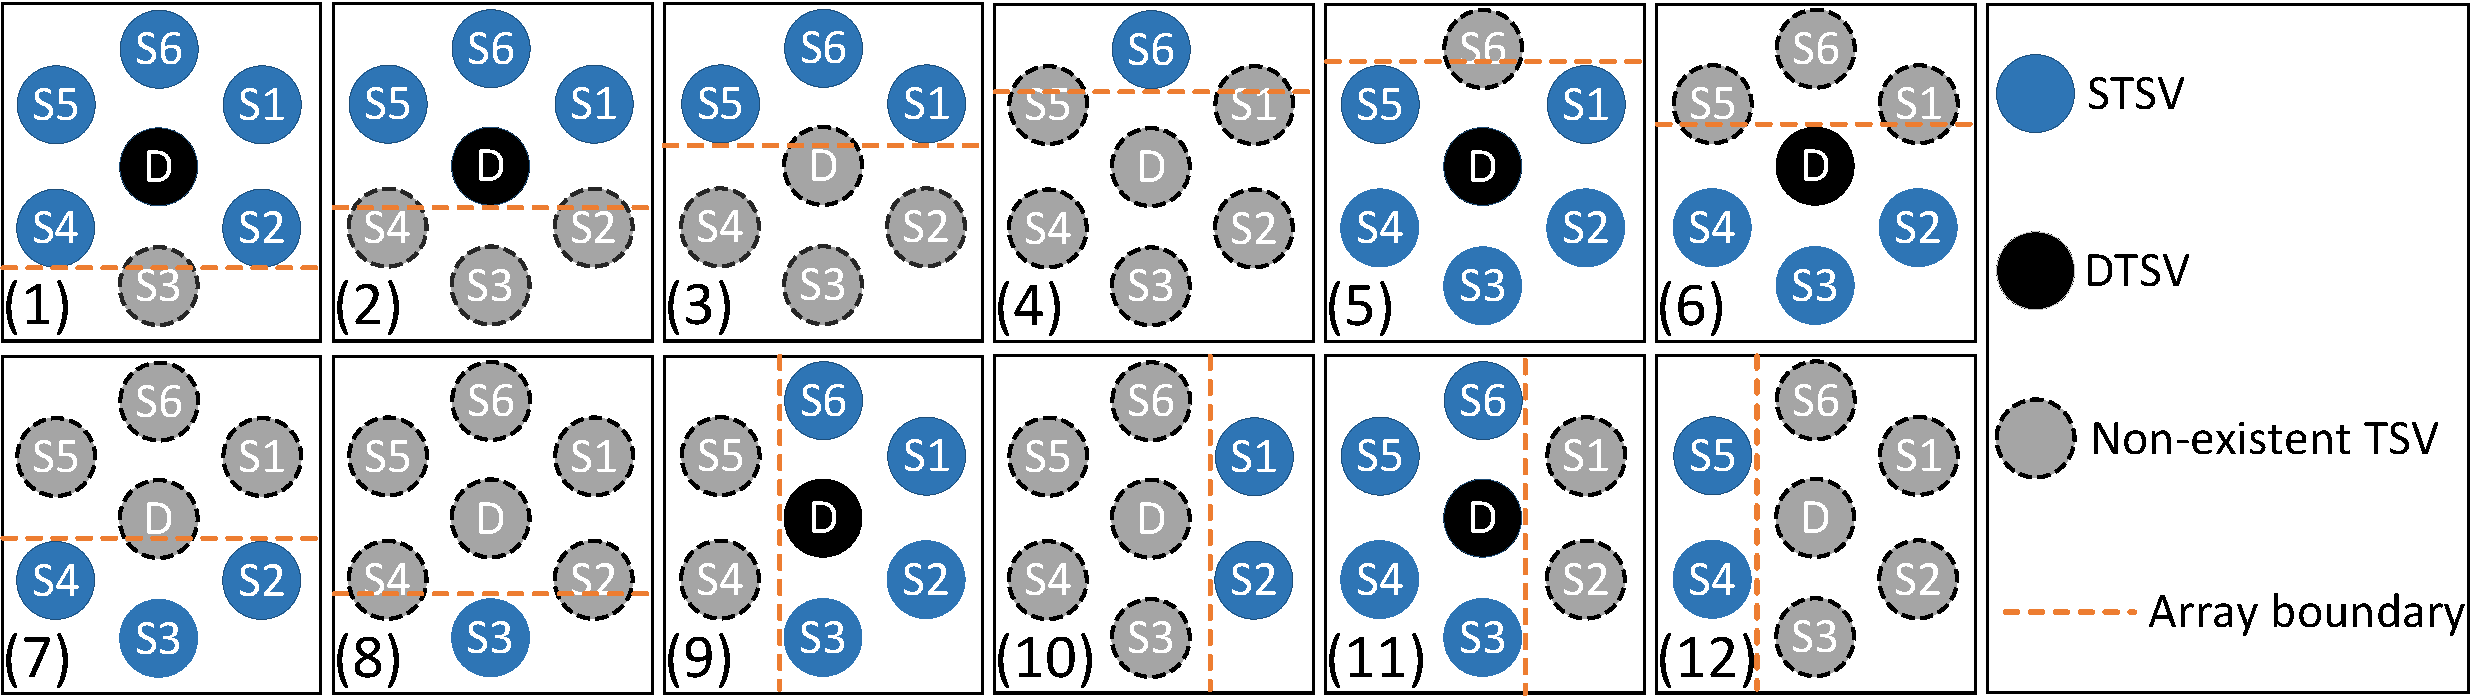
\includegraphics[width=3.4in]{./fig_files/fig_5.3.1.pdf}
	\caption{The examples of incomplete encoding groups. Sub-figures (1) to (10) illustrate different boundary conditions, in which the TSVs that do not actually exist are colored gray.}
	\label{fig-5.3.1}
\end{figure}

%\begin{table}
%	\renewcommand{\arraystretch}{1.1}
%	\caption{The average probability that the STSVs are in the free state in single cycle.}
%	\label{table-5.3.1}
%	\centering
%	\begin{tabular}{|c|c|c|}
%		\hline
%		\textcolor{black}{{\bf Case No.}} & \textcolor{black}{{\bf The number of virtual TSVs}} & \textcolor{black}{{\bf Probability}} \\
%		\hline
%		/ & 0 & 82.35\% \\
%		\hline
%		(1) & 1 & 85.31\% \\
%		\hline
%		(5) & 1 & 83.79\% \\
%		\hline
%		(9) & 2 & 86.82\% \\
%		\hline
%		(11) & 2 & 84.47\% \\
%		\hline
%		(2) & 3 & 89.06\% \\
%		\hline
%		(6) & 3 & 85.68\% \\
%		\hline
%		(3) & 4 & 91.67\% \\
%		\hline
%		(7) & 4 & 85.42\% \\
%		\hline
%		(10) & 5 & 87.5\% \\
%		\hline
%		(12) & 5 & 87.5\% \\
%		\hline
%		(4) & 6 & 100\% \\
%		\hline
%		(8) & 6 & 100\% \\
%		
%		\hline
%	\end{tabular}
%\end{table}

\begin{table}[!t]
	\renewcommand{\arraystretch}{1.0}
	\caption{The average probability that the STSVs are in the free state in single cycle.}
	\label{table-5.3.1}
	\centering
	\begin{tabular}{|c|c|c|}
		\hline
		\textbf{The number of virtual TSVs} & \textbf{Case No.} & \textbf{Probability} \\
		\hline
		0 & /         & 82.35\% \\
		\hline
		1 & (1), (5)  & 85.31\%, 83.79\% \\
		\hline
		2 & (9), (11) & 86.82\%, 84.47\% \\
		\hline
		3 & (2), (6)  & 89.06\%, 85.68\% \\
		\hline
		4 & (3), (7)  & 91.67\%, 85.42\% \\
		\hline
		5 & (10), (12)& 87.5\%, 87.5\% \\
		\hline
		6 & (4), (8)  & 100\%, 100\% \\
		\hline
	\end{tabular}
\end{table}

The results in Table \ref{table-5.3.1} validate that the probability of a STSV in the free state increases when it is categorized into the incomplete encoding group. Therefore, the code efficiency in a practical TSV array is higher than the estimation result obtained in Part \ref{subsec-code_rate-further_simp}. Moreover, as the array size expands, the proportion of TSVs located at the boundary in the total number of TSVs decreases. So the code efficiency is anticipated to gradually decrease with the increase of the array size and gradually approach the estimated value obtained in Part \ref{subsec-code_rate-further_simp}. These conclusions are verified in Part \ref{subsec-simu-bh}.

\section{Evaluation}\label{sec-simu}
\subsection{Crosstalk suppression capability}\label{subsec-simu-xtalk}
As discussed in Part \ref{subsec-dysh-layout}, for each STSV in Fig. \ref{fig-dysh_layout}(a), there are at most four directly adjacent aggressor TSVs (including three aggressor STSVs and one aggressor DTSV on the non-shielding state) having the signal transition that is opposite to it in a transmission cycle. Therefore, in the layout scheme proposed in Part \ref{subsec-dysh-layout}, the maximum crosstalk suffered by the STSVs is reduced from 12C level to 10C level.

Based on the layout scheme proposed in Part \ref{subsec-dysh-layout}, the CAC scheme proposed in Section \ref{sec-bscac} achieves a further reduction in the maximum crosstalk suffered by the STSVs. In the proposed CAC scheme, each STSV is allocated into an encoding group, and the signal on it remains unchanged if it is in the locked state. This reduces the maximum crosstalk suffered by each victim STSV from its three aggressor TSVs of the same encoding group, abbreviated as the intra-group aggressors, by at least $2\lambda C_{\rm L}$, i.e., from 6C level to no more than 4C level. The proof is presented in the following cases.

{\bf Case 1:} The signal value transmitted by the victim STSV in cycle $T$ is the same as that in cycle $T-1$. The crosstalk suffered by this victim STSV from its three intra-group aggressor TSVs is no more than $1\lambda C_{\rm L}+1\lambda C_{\rm L}+1\lambda C_{\rm L}=3\lambda C_{\rm L}$ according to formula (\ref{eq-xtalk_level_calc}). Fig. \ref{fig-6.1.1}(a) shows an example of this case.

\begin{figure}[t]
	\centering
	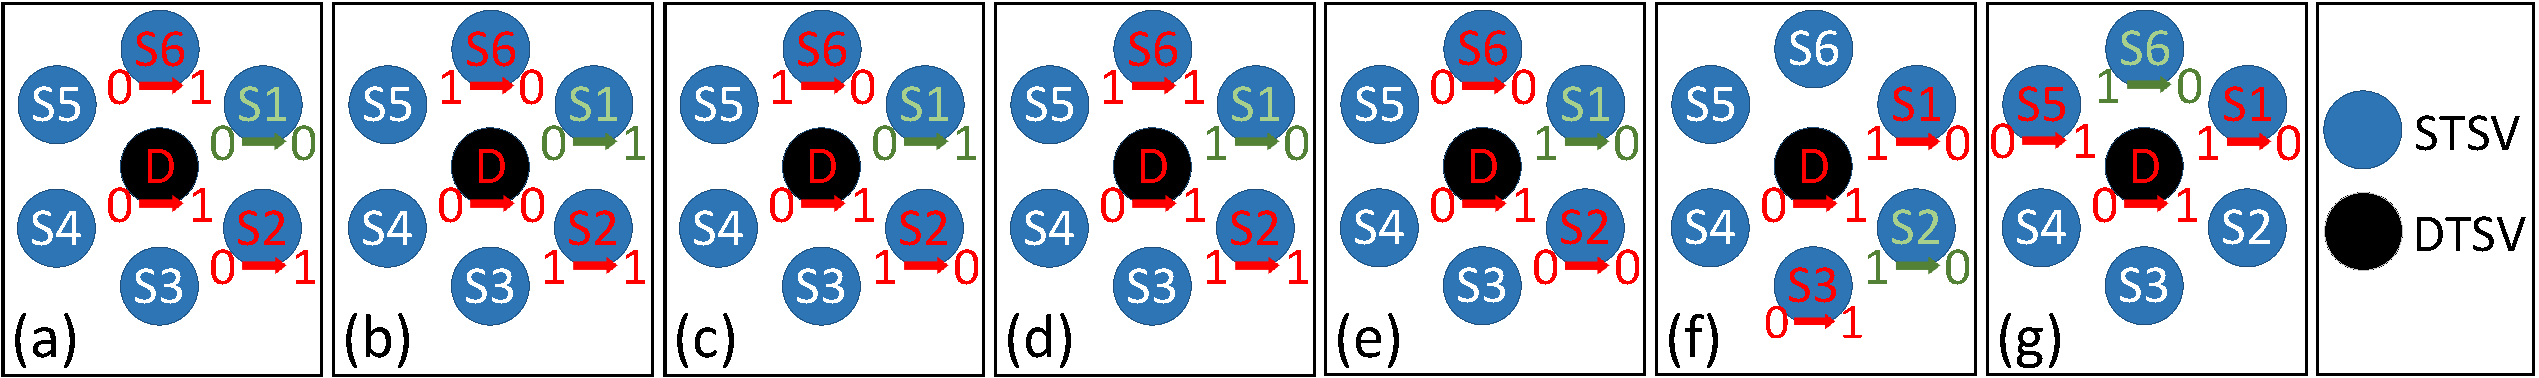
\includegraphics[width=3.5in]{./fig_files/fig_6.1.1.pdf}
	\caption{Some examples of the victim STSV suffers the crosstalk from its intra-group aggressor TSVs. The symbols of the victim STSVs are marked in green, and the symbols of the intra-group aggressor TSVs are marked in red.}
	\label{fig-6.1.1}
\end{figure}

{\bf Case 2:} The signal value transmitted by the victim STSV in cycle $T$ is different from that in cycle $T-1$, and the signal value on the intra-group DTSV of this victim STSV remains unchanged. At least one intra-group STSV is not allowed to have the signal transition opposite to this victim STSV according to Algorithm \ref{alg-bscac}. Therefore, the crosstalk suffered by this victim STSV from its three intra-group aggressor TSVs is no more than $1\lambda C_{\rm L}+1\lambda C_{\rm L}+2\lambda C_{\rm L}=4\lambda C_{\rm L}$. Fig. \ref{fig-6.1.1}(b) shows an example of this case.

{\bf Case 3:} The signal value transmitted by the victim STSV in cycle $T$ is different from that in cycle $T-1$, and the signal value on the intra-group DTSV of this victim STSV has a transition. The Case 2 in Part \ref{subsec-bscac-alg} is met, and this victim STSV satisfies at least one of the Conditions 2-1$\sim$2-5. 

{\bf Case 3-1:} If this victim STSV satisfies the Condition 2-1 in Part \ref{subsec-bscac-alg}, the crosstalk level suffered by it from its intra-group DTSV is $0\lambda C_{\rm L}$. Therefore, the crosstalk suffered by this victim STSV from its three intra-group aggressor TSVs is no more than $2\lambda C_{\rm L}+2\lambda C_{\rm L}+0\lambda C_{\rm L}=4\lambda C_{\rm L}$. Fig. \ref{fig-6.1.1}(c) shows an example of this case.

{\bf Case 3-2:} If this victim STSV satisfies the Condition 2-2 in Part \ref{subsec-bscac-alg}, the signal transition that has an opposite direction from that on this victim STSV cannot occur on its two intra-group aggressor STSVs. Therefore, the crosstalk suffered by this victim STSV from its three intra-group aggressor TSVs is no more than $1\lambda C_{\rm L}+1\lambda C_{\rm L}+2\lambda C_{\rm L}=4\lambda C_{\rm L}$. Fig. \ref{fig-6.1.1}(d) shows an example of this case.

{\bf Case 3-3:} If this victim STSV satisfies the Condition 2-3 in Part \ref{subsec-bscac-alg}, the signals on its two intra-group aggressor STSVs remain unchanged. Therefore, the crosstalk suffered by this victim STSV from its three intra-group aggressor TSVs is no more than $1\lambda C_{\rm L}+1\lambda C_{\rm L}+2\lambda C_{\rm L}=4\lambda C_{\rm L}$. Fig. \ref{fig-6.1.1}(e) shows an example of this case.

{\bf Case 3-4:} If this victim STSV satisfies Condition 2-4 or Condition 2-5 in Part \ref{subsec-bscac-alg}, there is one intra-group aggressor STSV exhibiting the same signal transition. Therefore, the crosstalk suffered by this victim STSV from its three intra-group aggressor TSVs is no more than $0\lambda C_{\rm L}+2\lambda C_{\rm L}+2\lambda C_{\rm L}=4\lambda C_{\rm L}$. Figs. \ref{fig-6.1.1}(f) and \ref{fig-6.1.1}(g) show two examples of this case.

To corroborate the above analysis, a $12\times 9$ hexagonal TSV array is taken as an instance to evaluate the crosstalk suppression capability of the proposed method. The crosstalk levels suffered by the STSVs in this hexagonal array are simulated over ten million transmission cycles. And the following four datasets are applied to the array in each cycle. (1) The data transmitted in each cycle consists of twelve 9-bit FNS-FPF-CAC codewords which are mapped to the TSVs row-by-row. (2) The data transmitted in each cycle consists of twelve 9-bit FNS-FTF-CAC codewords which are mapped to the TSVs row-by-row. (3) The data transmitted in each cycle consists of eighteen 6-bit FNS-CATF-CAC codewords. (4) The data transmitted in each cycle are generated by the proposed method.

The simulation results are shown in Fig. \ref{fig-6.1.2}. The existing FTF/FPF-CAC with row-by-row mapping reduces the maximum crosstalk from 12C to 10C, and the FNS-CATF-CAC further reduces it to 9C, whereas the proposed scheme further reduces it to 8C.

\begin{figure}[t]
	\centering
	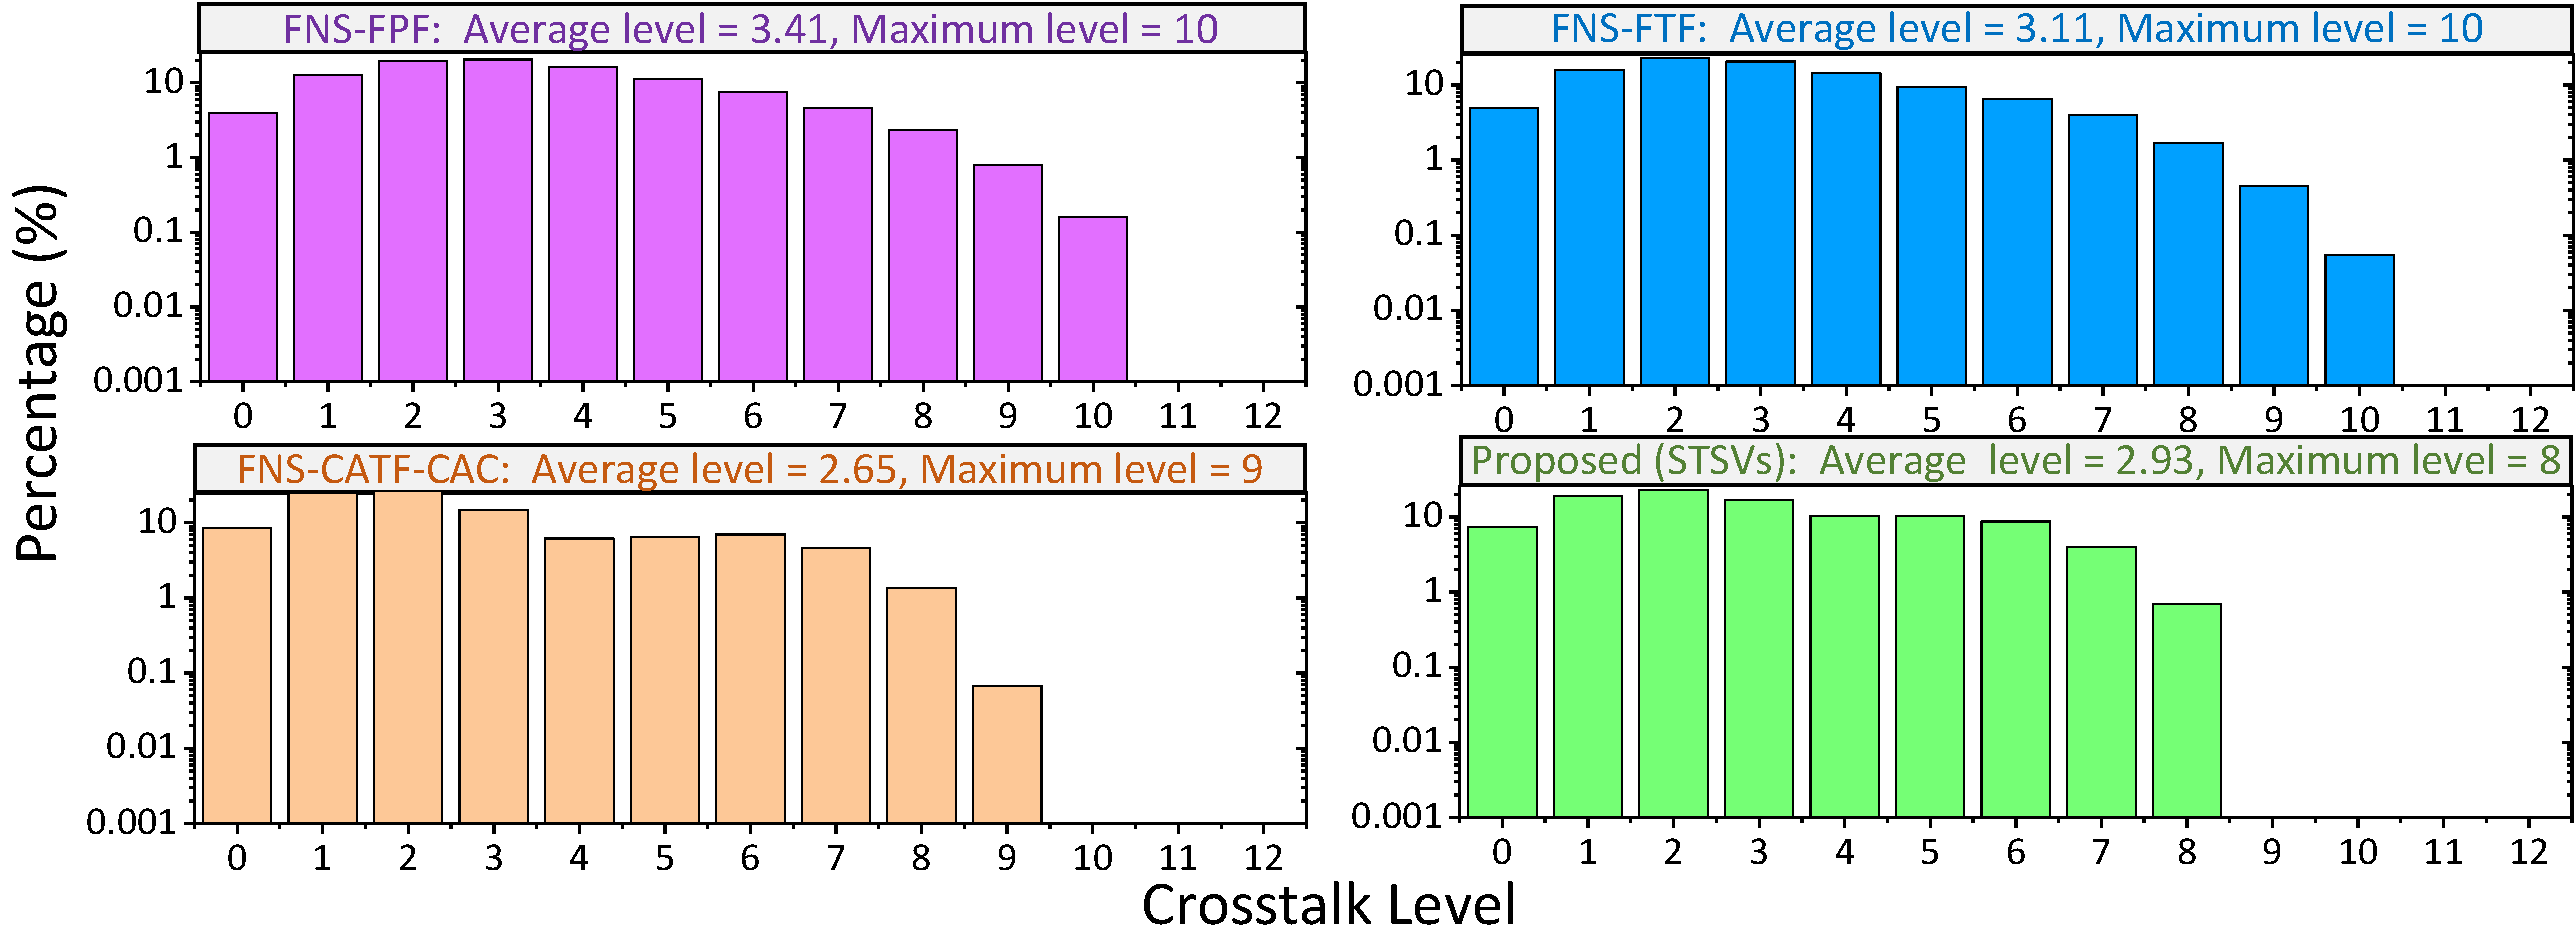
\includegraphics[width=3.45in]{./fig_files/xtalk01-n.pdf}
	\caption{The statistical results of the STSV crosstalk in the $12\times 9$ hexagonal array. The number $n\in [0, 12]$ on the horizontal coordinate axis indicates that the crosstalk level is $n$C.}
	\label{fig-6.1.2}
\end{figure}

The existing FTF/FPF-CAC methods are designed on the premise that the maximum crosstalk suffered by the edge TSVs is sufficiently low, as edge TSVs have fewer adjacent aggressors. However, when the edge effect is considered, the crosstalk suffered by the edge TSVs may exceed the expectation. In contrast, the crosstalk suppression capabilities of both the proposed scheme and the FNS-CATF-CAC method are barely affected by the edge effect. Assume that the edge TSVs in the $12\times 9$ hexagonal array suffer an additional grounding capacitance of $0.7\lambda C_{\rm L}$, and the ratio of the coupling capacitance between edge TSVs in the hexagonal arrays is 1.3 times that between non-edge TSVs \cite{A24_Bamberg_8106994,A25_BAMBERG201998}. Fig. \ref{fig-6.1.3} shows the crosstalk levels suffered by the STSVs in $12\times 9$ hexagonal array in the presence of edge effects. Compared with Fig. \ref{fig-6.1.2}, the maximum crosstalk level increases in the cases that the existing FTF/FPF-CAC methods are applied, but it keeps the same level in the case that the proposed scheme is applied.

\begin{figure}[t]
	\centering
	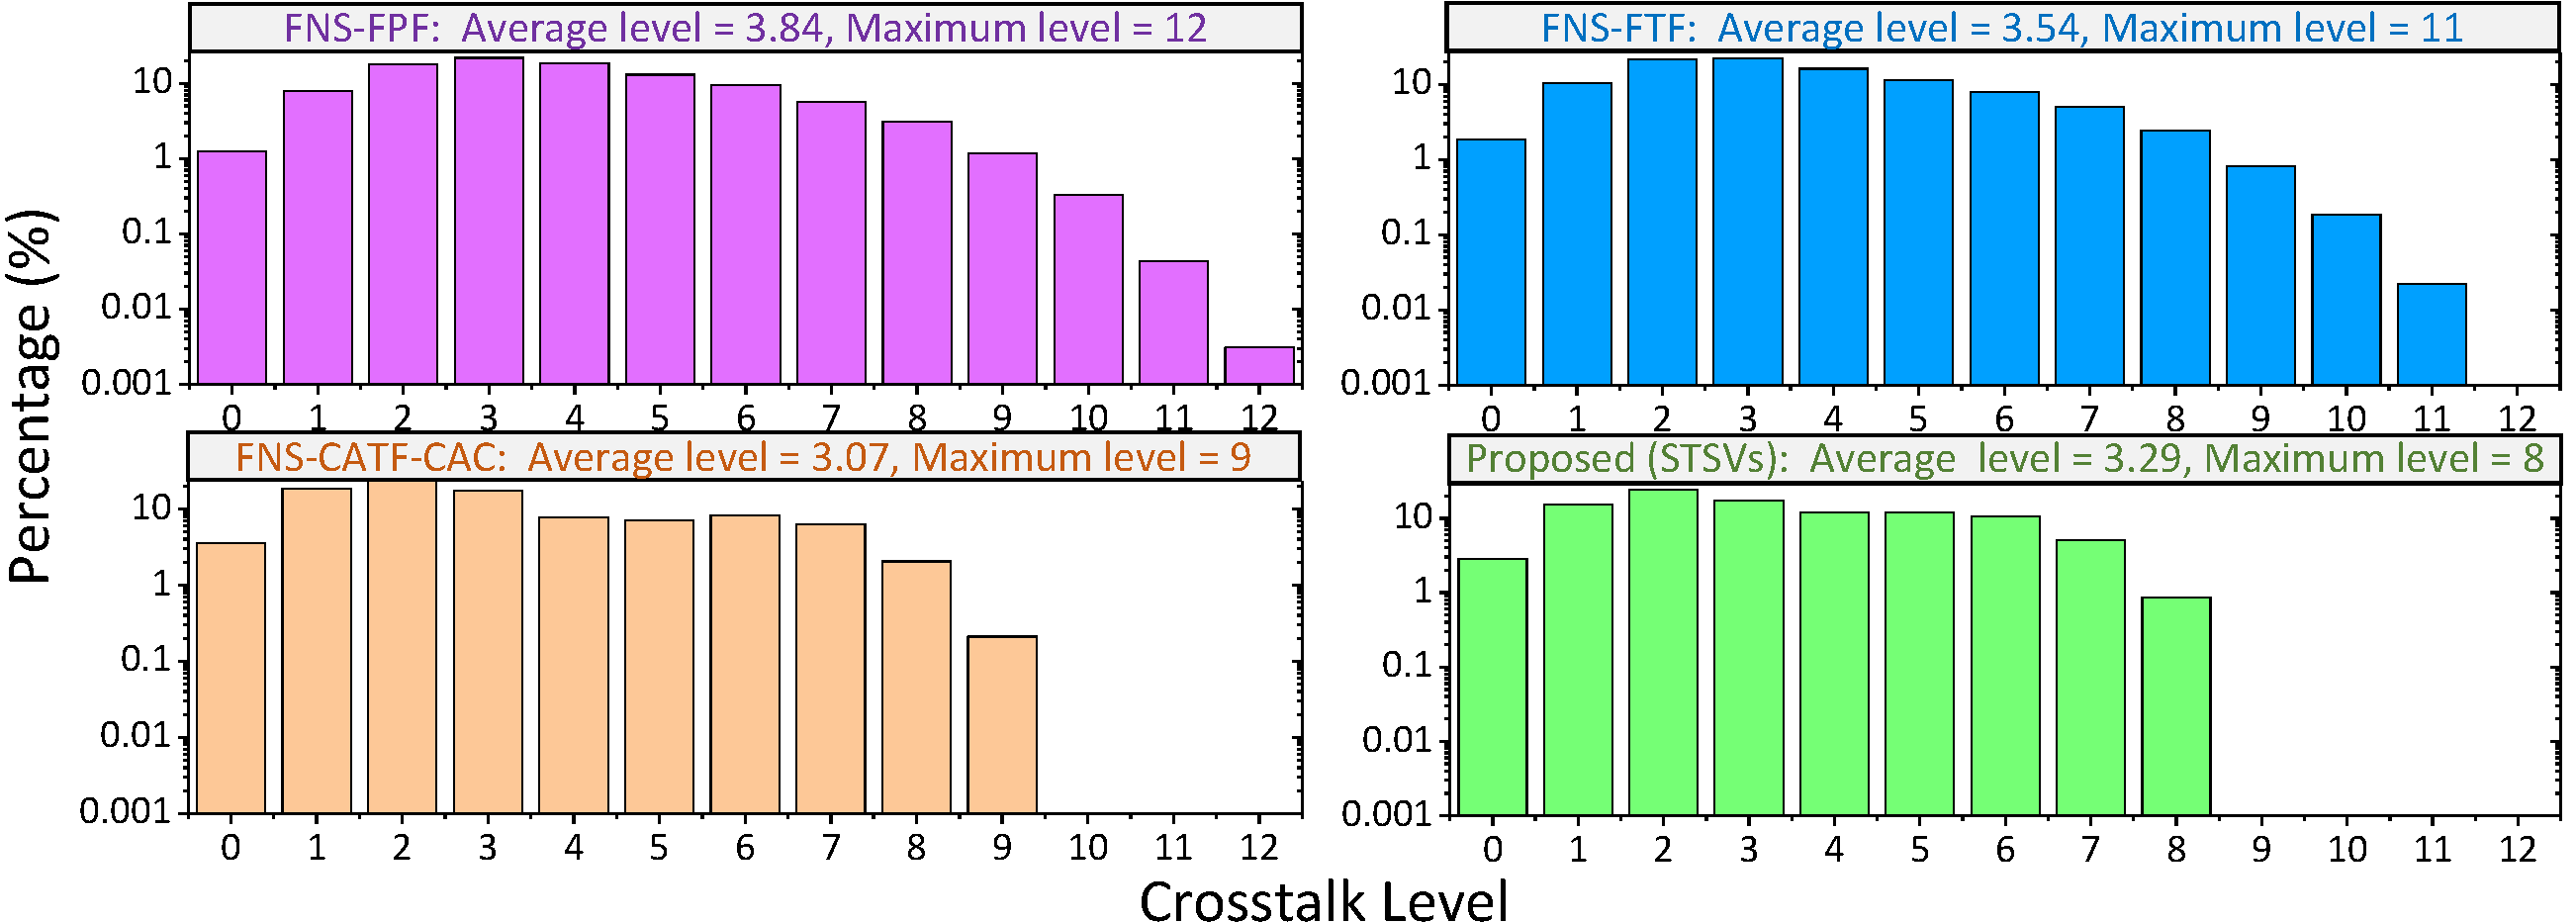
\includegraphics[width=3.45in]{./fig_files/xtalk02-n.pdf}
	\caption{The statistical results of the STSV crosstalk in the $12\times 9$ hexagonal array in the presence of edge effects. The number $n\in [0, 12]$ on the horizontal coordinate axis indicates that the crosstalk level is $n$C.}
	\label{fig-6.1.3}
\end{figure}

%The maximum crosstalk level in the TSV array limits the data transmission frequency, because it determines the maximum delay in the signal transmission. Although the transmissions with high-level crosstalk occupy a relatively low proportion as shown in Fig. \ref{fig-6.1.2} and Fig. \ref{fig-6.1.3}, designers cannot increase the signal transmission frequency because this may result in a significant increase in bit error rate. Fig. \ref{fig-6.1.4} shows the worst transition delay in different cases. The metal-insulator-semiconductor (MIS) transmission line TSV model\cite{A10_Cui_7851080,A29_Engin_6238321}, as shown in Fig. \ref{fig-6.1.4}(a) and (b), is used to simulate the transition delay.  $R_\text{TSV}$, $L_\text{TSV}$, $C_\text{TSV}$, $C_\text{i}$, $C_\text{c}$, $G_\text{c}$  and the load capacitance are $2\times 10^{-6} \Omega $, $1\times 10^{-11} \text{H}$, $2.1\times 10^{-15} \text{F}$, $1\times 10^{-12} \text{F}$, $1.2\times 10^{-14} \text{F}$, $1\times 10^{-2} \text{S}$ and $1\times 10^{-13} \text{F}$, respectively. The simulation is conducted with the Cadence Virtuoso IC6.1.7-64b, and each TSV is driven by an inverter in TSMC-N65 library. Fig. \ref{fig-6.1.4}(c) shows the simulation results. It proves the effectiveness of the proposed scheme in improving signal integrity.

%\begin{figure}[t]
%	\centering
%	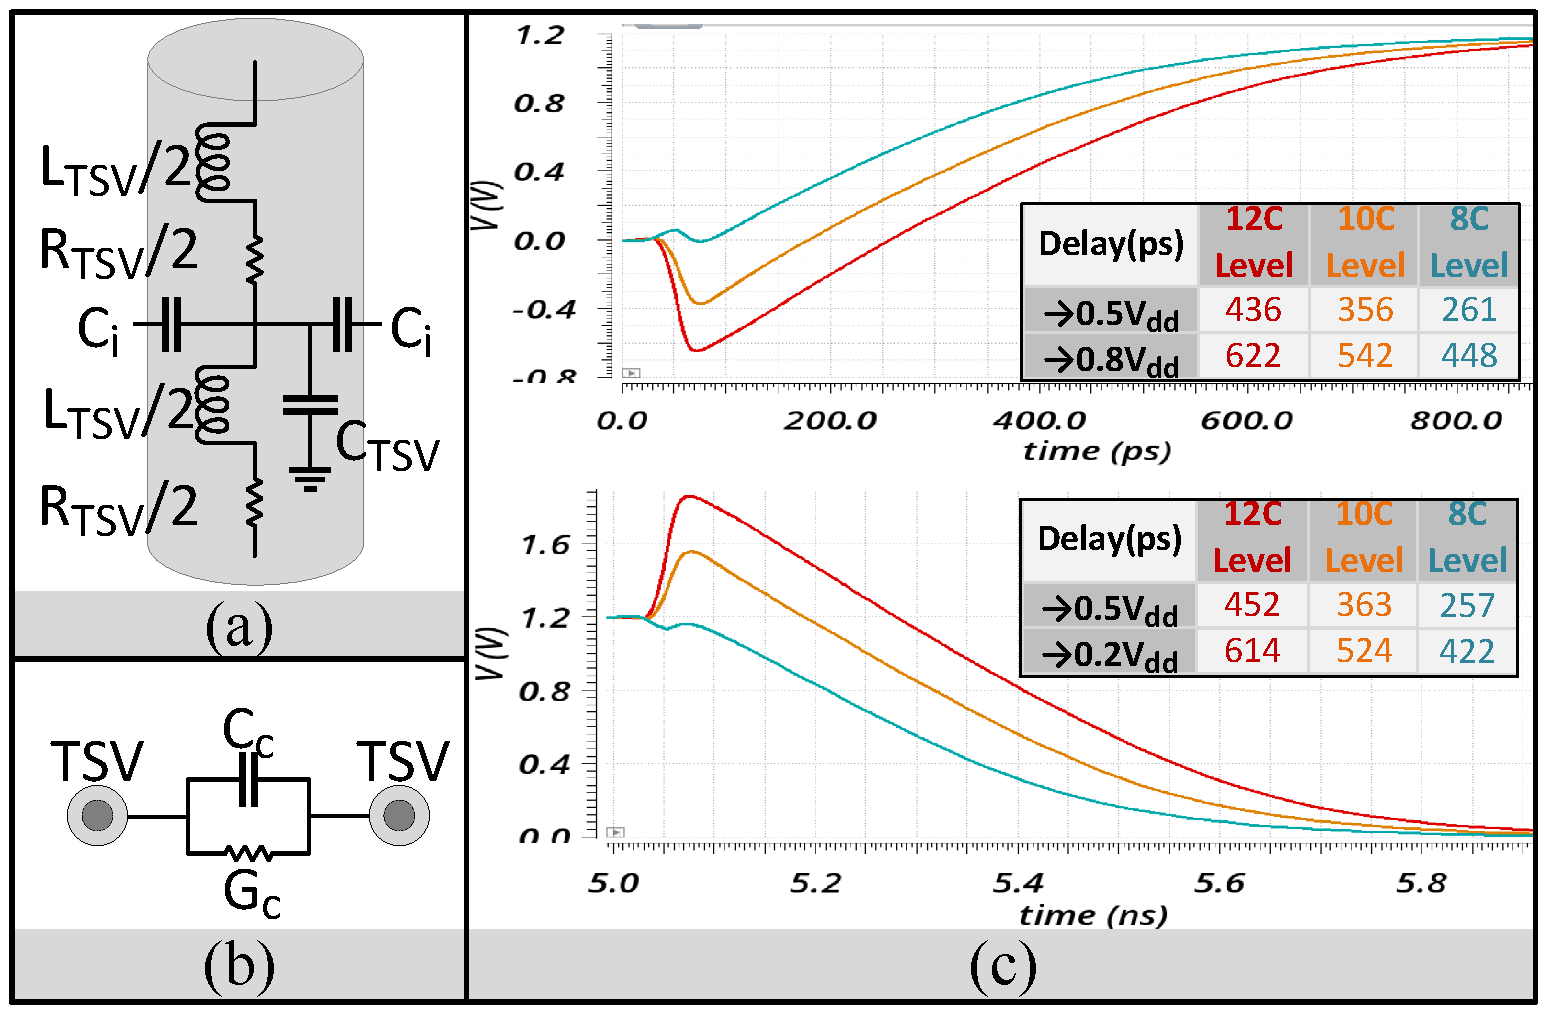
\includegraphics[width=3.0in]{./fig_files/TransitionDelay.pdf}
%	\caption{The worst transition delay of the victim TSV in hexagonal array. (a) and (b) show the metal-insulator-semiconductor (MIS) transmission line TSV model; (c) presents the simulation results.}
%	\label{fig-6.1.4}
%\end{figure}

\subsection{Bit overhead}\label{subsec-simu-bh}
The bit overhead is commonly used to evaluate the efficiency of crosstalk suppression solutions in TSV array. If at least $k$ TSVs are needed to transmit $w$-bit raw data, then the bit overhead $OH(k)$ is calculated as the following formula.

\begin{equation}
	OH(k) = (k-w)/w
	\label{eq-6.2.1}
\end{equation}

The bit overhead is a complement measure of the code efficiency. As analyzed in Section \ref{sec-code_rate}, the code efficiency of the proposed scheme is expected to gradually decrease and approaches the minimum value which lies between 66.01\% and 67.19\%, as the array size increases. This means that as the array size increases, the bit overhead of the proposed scheme is expected to gradually increase and approaches the maximum value which lies between 48.83\% and 51.49\%. In order to validate this conclusion, the bit overhead of the proposed scheme in the $N\times N$ hexagonal arrays with different sizes are simulated. The number of transmission cycles in each simulation is one million, and the raw data to be transmitted is generated randomly. The results are shown in Fig. \ref{fig-bitOH}. 

\begin{figure}[t]
	\centering
	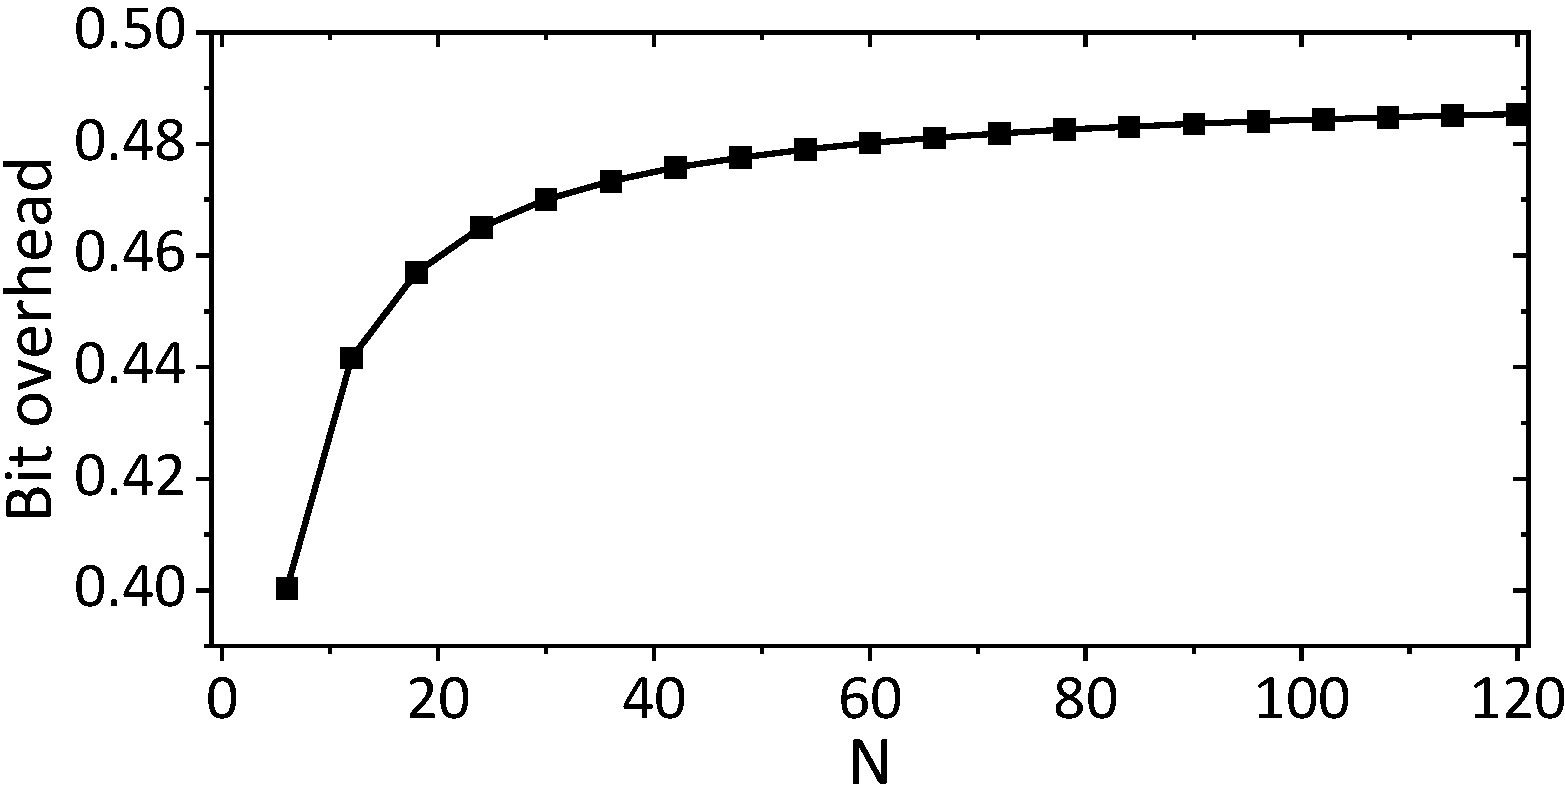
\includegraphics[width=1.8in]{./fig_files/BitOH.pdf}
	\caption{Simulation results for bit overhead in $N\times N$ hexagonal arrays.}
	\label{fig-bitOH}
\end{figure}

The results in Fig. \ref{fig-bitOH} corroborate the analysis in Section \ref{sec-code_rate}. For comparison, Table \ref{table-6.2.1} lists the bit overhead of some other CAC methods. The proposed scheme is one of the few CAC schemes applicable to hexagonal arrays of any size, along with the FTF/FPF-CAC schemes with row-by-row mapping and the FNS-CATF-CAC method. Compared with the FTF/FPF-CAC with row-by-row mapping and the FNS-CATF-CAC method, the proposed scheme achieves a significantly higher crosstalk suppression capability with a comparable bit overhead.

\begin{table*}
	\renewcommand{\arraystretch}{1.1}
	\caption{The comparison of different CAC schemes.}
	\label{table-6.2.1}
	\centering
	
	\begin{tabular}{|c|c|c|c|}
		\hline
		{\bf Scheme} & {\bf Application array types} & {\bf Crosstalk suppression capability} & {\bf Bit overhead} \\
		\hline
		FNS-CAC with shielding\cite{A20_Ran_7588317}
 & Three-row rectangular arrays only & 5.5C reduction & $\geq$80\% \\
		\hline
		3D-LAT ($w=4$) \cite{A19_Zou_6742982}
 & Three-row rectangular arrays only & 4C reduction & $>$60\% \\
		\hline
		3D-DyCAC \cite{A30_Shirmohammadi_8167468} & Three-row rectangular arrays only & 2.5C reduction & $\geq$71\% \\
		\hline
		6CmFNS \cite{A10_Cui_7851080}
 & Three-row rectangular arrays only & 4C reduction & $\geq$50\% \\
		\hline
		Mosaic-3C1S with TNS codec \cite{A11_Cui_9509749}
 & Rectangular arrays of any size & 4C reduction & 25\%$\sim$45\% \\
		\hline
		FTF/FPF-CAC with row-by-row mapping \cite{A31_Duan_4773140,A32_Duan_4555963}
 & Rectangular and hexagonal arrays of any size & 2C reduction & $\approx$45\% \\
 	    \hline
 FNS-CATF-CAC \cite{FNSCATF_10945736}
 & Rectangular and hexagonal arrays of any size & 3C reduction (hexagonal) & $\approx$45\% \\
		\hline
		Proposed & Hexagonal arrays of any size & 4C reduction & 40\%$\sim$51.5\% \\
		\hline
	\end{tabular}
	
\end{table*}

\subsection{Hardware implementation}\label{subsec-simu-hardware}
Compared with the CAC schemes based on specific numeral systems, such as FTF/FPF-CAC, the proposed scheme exhibits distinct differences in terms of hardware implementation. Fig. \ref{fig-r1-codec_impl_cmp} shows the application examples of FTF/FPF-CAC scheme, FNS-CATF-CAC scheme and the proposed scheme in the TSV arrays. In the given examples, the FIFO (First-In First-Out) modules are employed to store the logic values waiting to be transmitted on the source side and the logic values received from each TSV on the sink side. The symbols $\rm clk\_tx$ and $\rm clk\_rx$ are the same-frequency clock signals at the source and sink sides, respectively. The symbols $\rm en\_tx$ and $\rm en\_rx$ are the read-enable signal and write-enable signal of the FIFOs.

\begin{figure}[t]
	\centering
	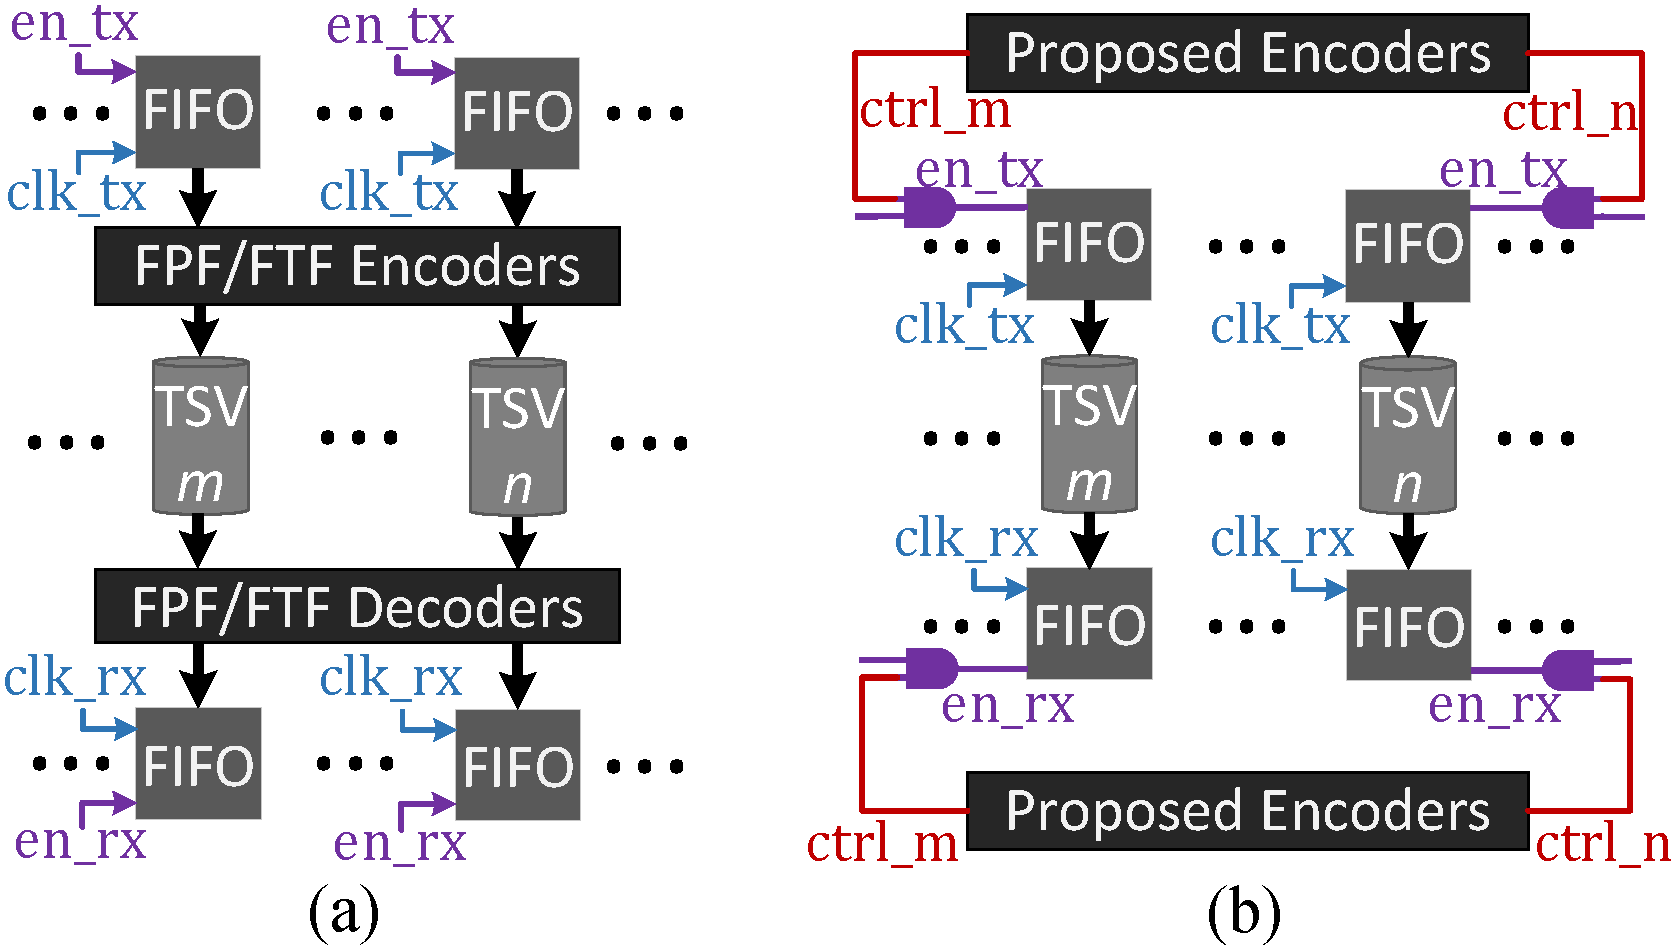
\includegraphics[width=2.3in]{./fig_files/Codec_inplementation_compare.pdf}
	\caption{Examples of the application of (a) FTF/FPF-CAC scheme and FNS-CATF-CAC scheme, and (b) the proposed scheme in the TSV arrays.}
	\label{fig-r1-codec_impl_cmp}
\end{figure}

In Fig. \ref{fig-r1-codec_impl_cmp}(a), which applies the FPF/FTF-CAC scheme, the raw data is first converted into codeword sequences by the encoders, transmitted through the TSV array, and then recovered at the sink side by the decoders. Since the bitwidth of each codeword is larger than that of the corresponding raw data, the number of TSVs is greater than that of the FIFO modules at the source/sink side. A similar codec structure is also adopted in the FNS-CATF-CAC scheme.

In contrast, the proposed scheme does not directly modify the data to be transmitted through encoders, so the number of TSVs is equal to that of the FIFO modules on source/sink side. Instead, it generates control signals capable of pausing the transmission process on certain TSVs according to the raw data, as shown in Fig. \ref{fig-r1-codec_impl_cmp}(b). Assume that ${\rm TSV}_m$ is a DTSV and ${\rm TSV}_n$ is an STSV. If the DTSV ${\rm TSV}_m$ is in the shielding state, the control signal $\rm ctrl\_m$ generated by the proposed encoder is 0, which locks the read-enable signal $\rm en\_tx$ of the corresponding FIFO on the source side to 0, and locks the write-enable signal $\rm en\_rx$ of the corresponding FIFO on the source side to 0. If the DTSV ${\rm TSV}_m$ is in the non-shielding state, the control signal $\rm ctrl\_m$ is 1. If the STSV ${\rm TSV}_n$ is in the locked state, the control signal $\rm ctrl\_n$ generated by the proposed encoder is 0; otherwise, $\rm ctrl\_n$ is 1. In this way, all the DTSVs in the shielding state and the STSVs in the locked state keep the logic values they transmit invariant.

It should be noted that Fig. \ref{fig-r1-codec_impl_cmp} is merely an example and does not imply that the implementation of this scheme depends on the FIFO modules. For example, in the design using the simplest D flip-flops rather than FIFOs to apply and capture the logic values on TSVs, the control signals generated by the proposed encoder can be used for the clock gating of the corresponding registers to achieve the expected results.

The encoder implementation of the proposed scheme, which is the crux of Fig. \ref{fig-r1-codec_impl_cmp}(b), mainly consists of the following parts.

{\bf (1) Control signal generation for DTSVs:} As shown in Fig. \ref{fig-dysh_layout}, there are three types of DTSVs in the proposed scheme, which are denoted as D1, D2 and D3. According to Fig. \ref{fig-dysh_layout}(b), the three 1-bit control signals for D1-type, D2-type and D3-type DTSVs can be generated by three 1-bit registers.

%\begin{figure}[t]
%	\centering
%	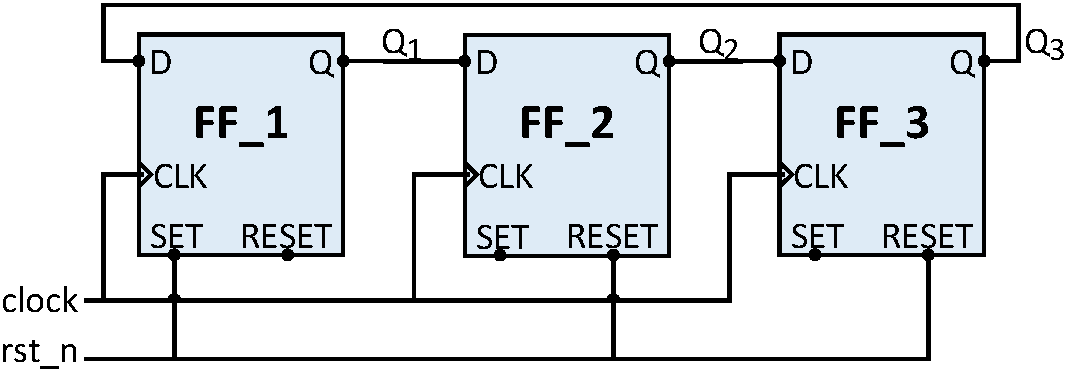
\includegraphics[width=2.3in]{./fig_files/CtrlSignalGen_DTSV.pdf}
%	\caption{The control signal generation circuit for DTSVs.}
%	\label{fig-r1-ctrlSigGen_DTSV}
%\end{figure}

{\bf (2) Control signal generation for STSVs:} In each transmission cycle, any STSV in Fig. \ref{fig-dysh_layout} can be categorized into exactly one encoding group, and its state is determined by a BS-CAC encoder. Each BS-CAC encoder can generate the 1-bit control signals for at most six STSVs independently according to Algorithm \ref{alg-bscac}. As shown in Fig. \ref{fig-bscac_3groups}, there are three types of encoding groups, which are centered on the D1-, D2- and D3-type DTSVs, respectively. Assuming a sufficiently large hexagonal array contains $N$ TSVs, the number of BS-CAC encoders required is approximately $N/9$ according to Fig. \ref{fig-dysh_layout}. In addition, most STSVs require three 3-to-1/1-to-3 MUXer to switch among different encoding groups.

As is evident from the foregoing discussion, in the context of this proposed scheme, the area and power consumption overhead exhibit an approximate linear relationship with the scale of TSV array. Conversely, the delay scarcely varies with changes in the array size. Unfortunately, accurately evaluating the hardware overhead for arrays of diverse sizes poses a significant challenge. Firstly, the quantity of MUXers is not merely contingent upon the size of the array. It is intricately influenced by the specific details of coding group allocation and the specific circumstances at the array's boundaries. Secondly, as expounded upon in Part \ref{subsec-bscac-process}, the encoding procedures near the array boundaries are subject to varying levels of simplification. Consequently, the actual hardware overhead of the BS-CAC encoder is likewise affected by the boundary conditions of the array.

Therefore, this paper conducts simulations solely on the hardware overhead of BS-CAC encoders without considering the boundary conditions. Taking into account the following reasons, such a simplification will not give rise to substantial deviations. Firstly, the overhead of MUXers and three 1-bit registers is negligible compared with that of the BS-CAC encoders. Secondly, although ignoring the MUXers would lead to a slightly underestimated hardware cost, ignoring the boundary conditions would simultaneously result in a slightly overestimated hardware cost.

The proposed BS-CAC encoder design is synthesized with the Semiconductor Manufacturing International Corporation (SMIC) 65nm technology file by the Design Compiler tool. Firstly, with the maximum timing-optimization constraint applied, i.e., applying the constraint with a very small clock period to enable the Design Compiler to optimize the delay as much as possible, the delay of the BS-CAC encoder is 1.04$\rm ns$. This value remains unaffected by the size of the array. By contrast, Fig. \ref{fig-r1-hardware_overhead}(a) shows the delay of the FNS-FTF/FPF-CAC and FNS-CATF-CAC codecs under the same design constraints. It can be observed their delay values exhibit an upward trend as the codeword bitwidth expands. Hence, with the continuous growth of the array size, the superiority of this scheme in terms of delay becomes increasingly prominent.

Then, an evaluation is conducted on the area and power consumption of the BS-CAC encoder and several other CAC codecs. To ensure a fair comparison, the clock period is set to 10$\rm ns$ to prevent the area of some designs from increasing as a result of stringent timing constraints. The area and power consumption of each BS-CAC encoder are approximately 27.04$\rm um^2$ and 0.00172$\rm mW$ per TSV. The area and power consumption per TSV remains almost unchanged as the array scale expands. By contrast, Fig. \ref{fig-r1-hardware_overhead}(b) and (c) show the area and power consumption per TSV of the FNS-FTF/FPF-CAC  and the FNS-CATF-CAC codecs under the same constraints, which can be observed that the area and power consumption per TSV exhibit an upward trend as the codeword bitwidth expands. Hence, with the continuous growth of the array size, the advantage of this scheme in terms of area and power consumption becomes more and more obvious.

\begin{figure}[t]
	\centering
	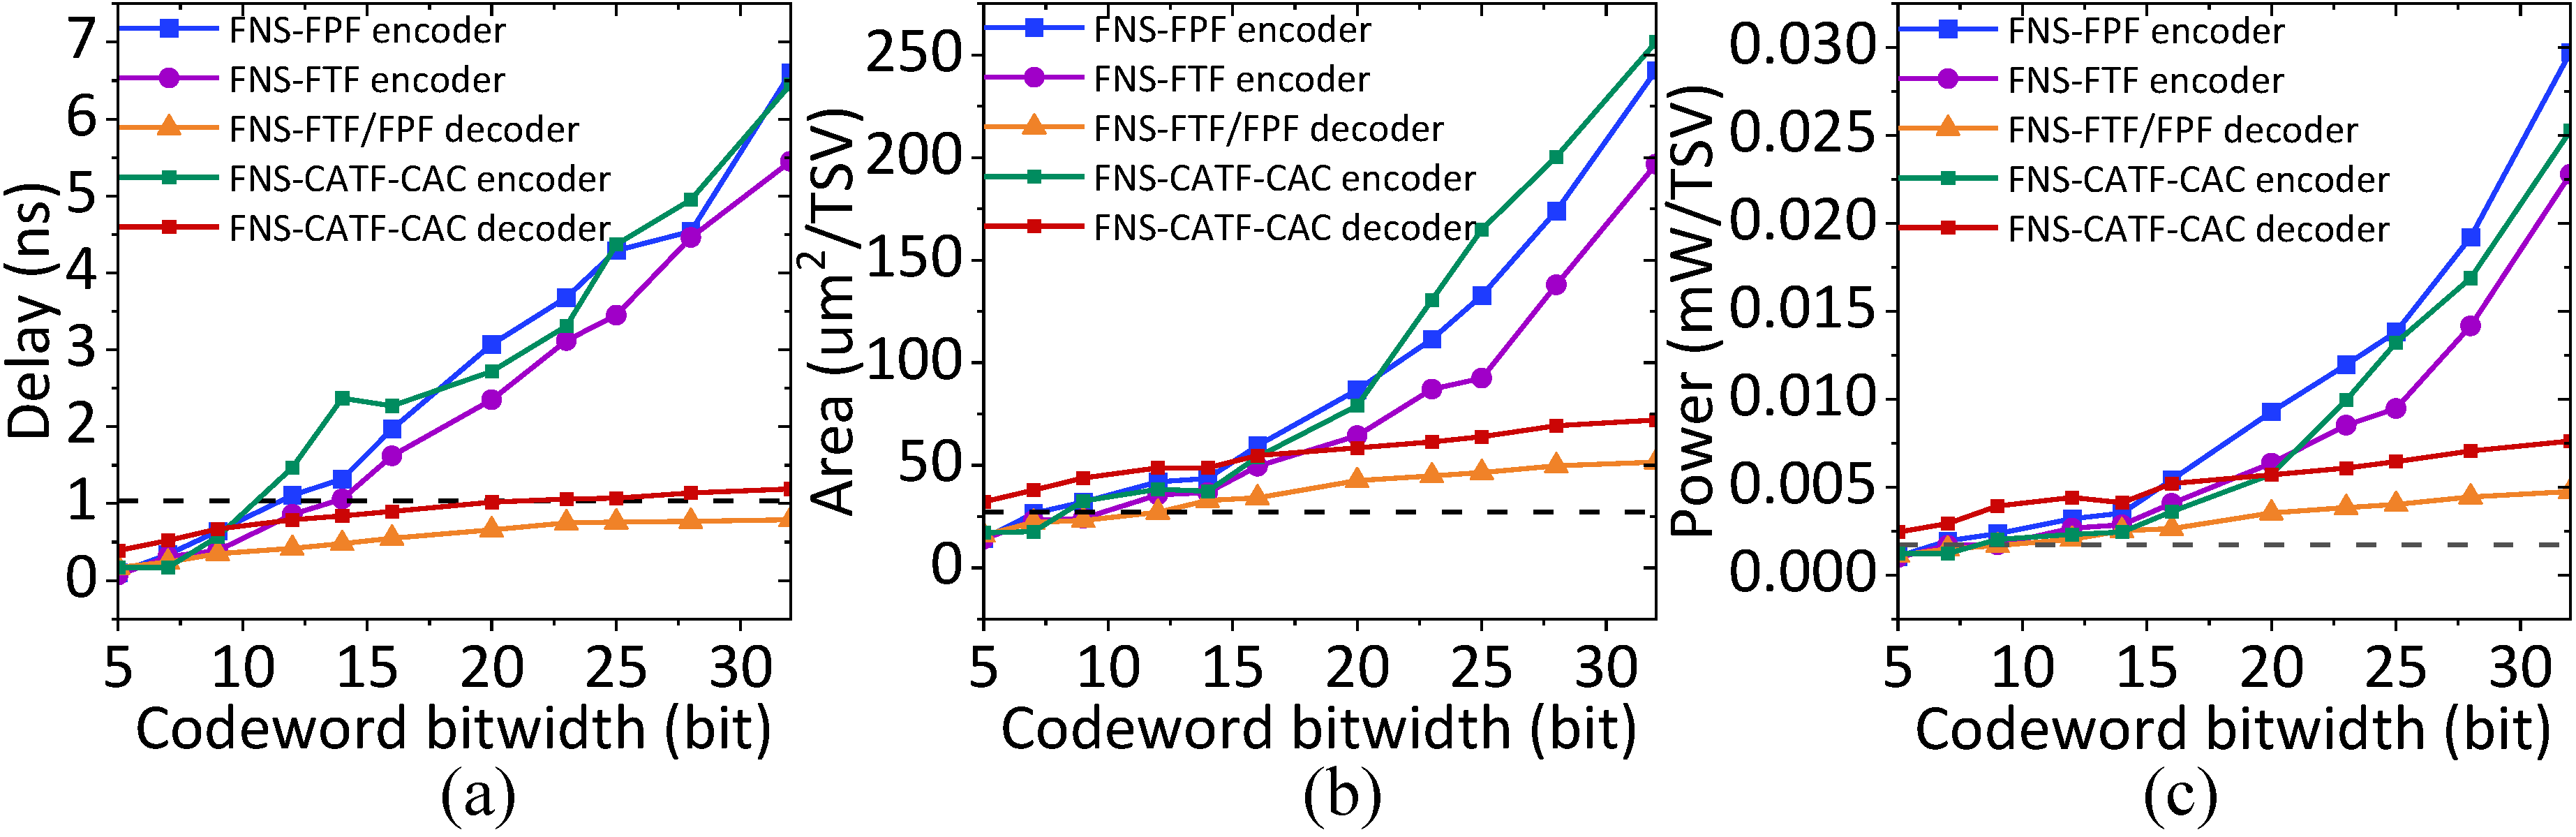
\includegraphics[width=3.5in]{./fig_files/HardwareOverhead.pdf}
	\caption{A comparison of different codecs in terms of (a) delay, (b) average area per TSV, and (c) average power per TSV. The black dotted line represents the hardware overhead of BS-CAC.}
	\label{fig-r1-hardware_overhead}
\end{figure}


%\subsection{\textcolor{black}{Integration with UCIe}}\label{subsec-hw-ucie}
%
%\textcolor{black}{This subsection discusses the feasibility and benefits of integrating the proposed scheme with UCIe (Universal Chiplet Interconnect Express) standard\cite{R1-ucie}.}
%
%\textcolor{black}{Firstly, the proposed scheme has excellent compatibility with the UCIe, which is far superior to the existing CAC schemes based on specific numeral systems such as FTF/FPF-CAC. The primary reasons can be attributed to the following two aspects.}
%
%\textcolor{black}{(1) In UCIe standard, the interconnect redundancy remapping is adopted to improve the assembly yield and recover functionality. Take the $\times$64 advanced package module as an example, in which 64 data lanes are divided into two self-repair groups, and each self-repair group contains 32 data lanes and 2 additional redundant lanes. As shown in Fig. \ref{fig-r1-ucie_remapping}, the lanes within each group are interconnected in a specific order. In the event that a particular lane malfunctions, the data that was originally being transmitted through it can be redirected to an adjacent lane for transmission. However, this is highly likely to render the crosstalk suppression effect of the existing CAC schemes based on specific numeral systems ineffective. The reason is that the effectiveness of these existing schemes depends on mapping the generated codeword sequences to the TSV array according to specific rules, and the redundancy remapping mechanism may disrupt these specific rules. In comparison, the proposed scheme does not encode the raw data into codeword sequences. Consequently, there is no issue regarding the mapping rules between codeword sequences and the TSV array. Thus, the proposed scheme in this paper is fully compatible with the redundancy remapping mechanism in UCIe.}
%
%\begin{figure}[t]
%	\centering
%	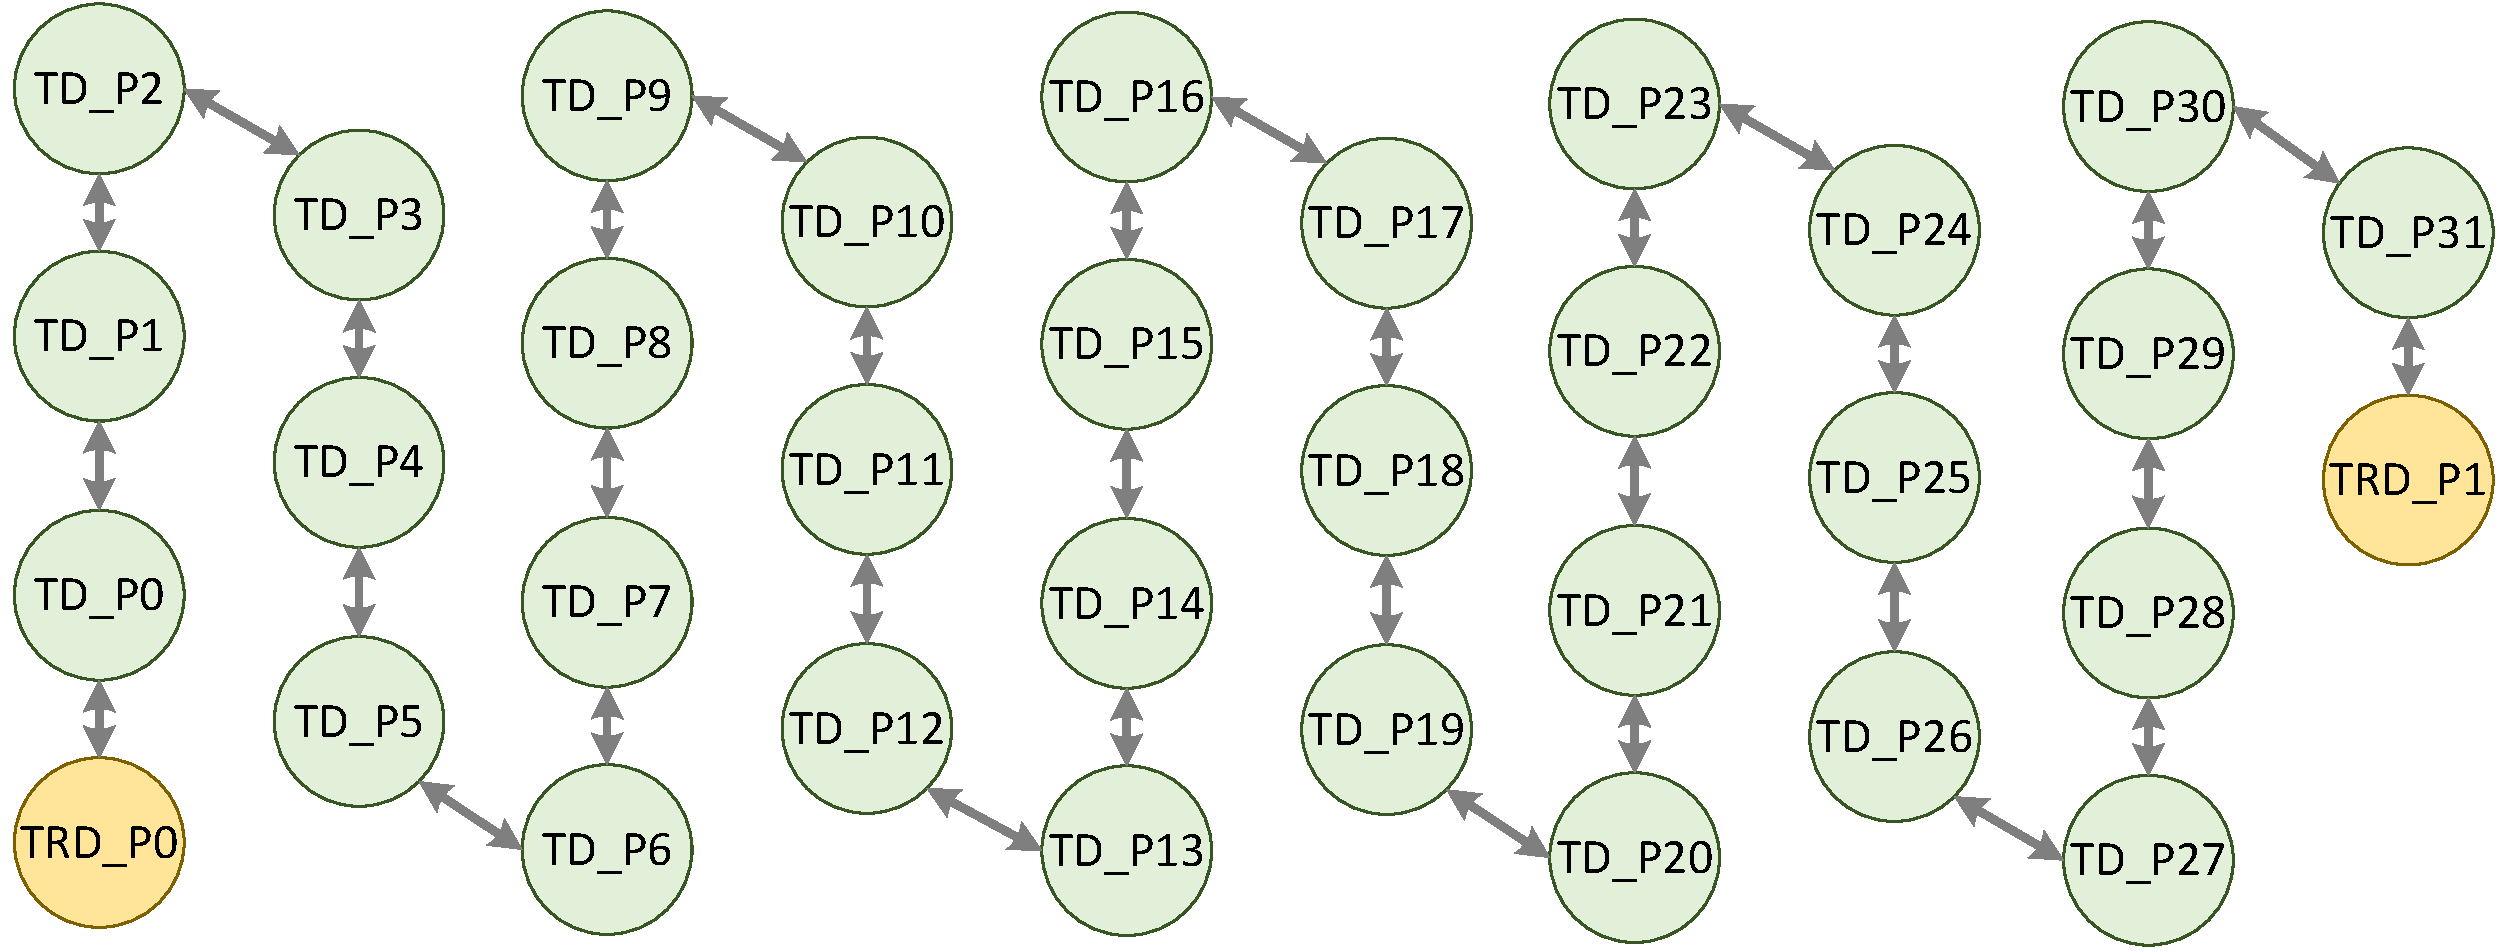
\includegraphics[width=3.3in]{./fig_files/UCIe_remapping.pdf}
%	\caption{\textcolor{black}{The interconnect redundancy remapping in the advanced package module of UCIe\cite{R1-ucie}.}}
%	\label{fig-r1-ucie_remapping}
%\end{figure}
%
%\textcolor{black}{(2) Taking the FTF/FPF-CAC as an example, in order to attain compatibility with the redundancy remapping mechanism in UCIe, the following conditions should, at a minimum, be satisfied\cite{A21_Wei_10224770,A22_Wei_9796564}. Firstly, The logic values transmitted by each self-repair group must come from the same one FTF/FPF encoder. Secondly, all redundant lanes within each group are positioned at the edges of the array. These conditions require the implementation of FTF/FPF-CAC codecs with a codeword bitwidth of at least 32 bits. Nevertheless, taking into account that the hardware overhead of FTF/FPF-CAC codecs increases rapidly and non-linearly as the codeword bitwidth expands, this is scarcely acceptable. As shown in Fig. \ref{fig-r1-hardware_overhead}, the hardware overhead of the 32-bit FNS-FTF/FPF-CAC codecs is several times that of the proposed BS-CAC encoder.}
%
%\textcolor{black}{Secondly, as a crosstalk suppression technique, the proposed scheme can effectively improve the data transmission reliability of TSV arrays. Although the UCIe standard have adopted some ECC (Error Correction Code) techniques to address the errors arising during the transmission process, including the bit flips induced by crosstalk, these ECC-based mechanisms are hard to be the alternative to the crosstalk suppression technique, as explained below.} 
%
%\textcolor{black}{Fig. \ref{fig-6.1.4} shows the comparison of signal transition with different crosstalk levels. It can be seen that the signal transition delay can be significantly reduced by using the proposed scheme to decrease the crosstalk level. The maximum transition delay limits the signal transmission rate. For example, if the signal transmission rate is set to 2.2GHz, then the data transmission with 12C-level crosstalk will cause errors. Because the period of 455ps only allows the signal to rise from 0 to approximately ${\rm V_{dd}}/2$, or fall from ${\rm V_{dd}}$ to approximately ${\rm V_{dd}}/2$. However, data transmission with 8C-level crosstalk can be completed correctly. Because the period of 455ps is sufficient to rise the signal from 0 to $\rm 0.8V_{dd}$ or drop the signal from $\rm V_{dd}$ to $\rm 0.2V_{dd}$. The proposed scheme is able to reduce the maximum transition delay by eliminating the data patterns which cause the high-level crosstalk, so as to enable the TSV to transmit data at a higher frequency, or to provide a higher tolerance threshold while maintaining the original transmission rate.}
%
%\textcolor{black}{The transmission errors that the crosstalk suppression schemes are designed to avoid are somewhat deterministic. These errors are caused by the data patterns with the high-level crosstalk and are therefore somewhat predictable. The high-level crosstalk slows down the rise or fall of signal, which causes the registers in the sink side to capture the wrong logic values. If the influences of random factors are not taken into consideration, the same data error can be reproduced if we repeat the same data transmission process. In contrast, the ECC mechanisms increase the minimum Hamming distance of the codeword set by adding additional check bits, which is intended to detect or correct the random error bits. In the discussions of ECC coding schemes, the term "error" usually refers to a $0\to 1$ or $1\to 0$ that cannot be predicted and is hard to reproduce. Therefore, the proposed scheme and the ECC mechanisms in UCIe standard are designed to cope with the different problems.}
%
%\textcolor{black}{In addition, the ECC mechanism in UCIe standard cannot replace the crosstalk suppression schemes to deal with the errors due to crosstalk in TSV arrays. Assume that the probabilities of the crosstalk levels in different TSVs are independent. Based on this assumption, in each transmission period, if the probability that the crosstalk-induced error occurs in one TSV is $p$, then the probability $P(X)$ that $X\in [0, N]$ error bits occur in the array containing $N$ signal TSVs is calculated by the following equation.}
%
%\begin{equation}
%	\textcolor{black}{P(X)={{\rm C}_N^X}(1-p)^{N-X}p^X}
%	\label{eq-R1-6.D.1}
%\end{equation}
%
%\textcolor{black}{Based on the result in Fig. \ref{fig-6.1.3}, Fig. \ref{fig-r1-ucie_errorPr} shows the probabilities of different number of errors occurring when the thresholds of crosstalk level causing bit errors are 9C, 10C and 11C. It should be noted that Fig. \ref{fig-r1-ucie_errorPr} shows the probabilities in only one transmission cycle. If the transmission speed is set to 2GHz, there are $2\times 10^9$ transmission cycles within one second. Obviously, this is far beyond the error correction capability of ECC mechanisms applied in UCIe standard.}
%
%\begin{figure}[t]
%	\centering
%	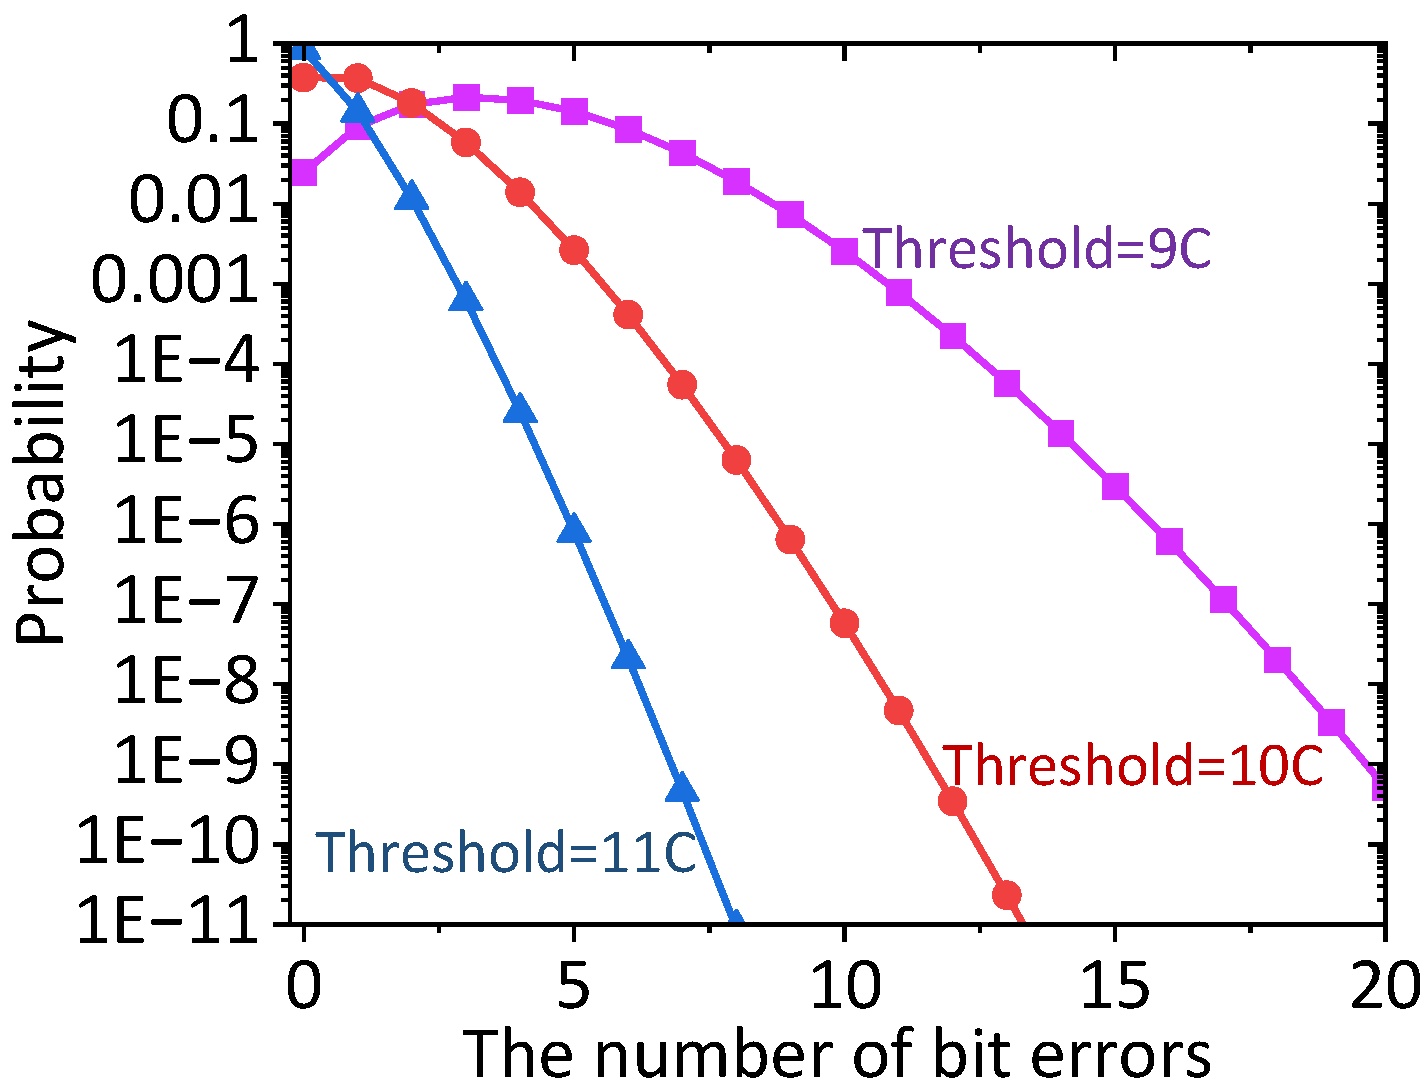
\includegraphics[width=2.1in]{./fig_files/BitErrorPr.pdf}
%	\caption{\textcolor{black}{The probabilities of different number of errors occurring when the thresholds of crosstalk level are 9C, 10C and 11C.}}
%	\label{fig-r1-ucie_errorPr}
%\end{figure}


\section{Conclusion}\label{sec-conclusion}
This paper proposes a crosstalk suppression scheme utilizing the dynamic shielding and bit-stuffing code techniques for hexagonal TSV arrays. 
%This is the first CAC-based crosstalk suppression scheme designed specifically for the hexagonal TSV arrays. 
Compared with the existing FTF/FPF-CAC and FNS-CATF-CAC schemes, the proposed scheme is a better choice for the following reasons. (1) The proposed scheme is able to reduce the inter-TSV crosstalk by 4C levels, whereas the FTF/FPF-CAC and FNS-CATF-CAC schemes reduce it by 2C and 3C levels, respectively. (2) The bit overhead of the proposed scheme is 40\%$\sim$51.5\%, which is comparable with that of the FTF/FPF-CAC and FNS-CATF-CAC schemes. (3) The hardware overhead of the proposed method is much lower than that of the existing FTF/FPF-CAC and FNS-CATF-CAC methods in the large-scale arrays.


{\appendix \label{sec-appendix}
%In Algorithm \ref{alg-encoding}, assume that $g_n=0$ and $g_1=g_2=1$, the value of variable $v$ is updated from 3 to 1 in the lines 12$\sim$17 with $i=2$, and the value of $g_3$ is 0 according to lines 13$\sim$14. The following statements can be deduced in turn.
%
%{\bf Statement 1:} In the lines 12$\sim$17 with $i=3$, $g_3$ is 0 if $v=f_4=3$. This indicates that $g_4=1$ and the value of $v$ is updated from $f_4+f_5=f_6=8$ to $f_4=3$ in the lines 12$\sim$17 with $i=4$. In the case that $g_4=1$, the value of $g_5$ is 0 according to lines 13$\sim$14.
%
%{\bf Statement 2:} In the lines 12$\sim$17 with $i=5$, $g_5$ is 0 if $v=f_6=8$. This indicates that $g_6=1$ and the value of $v$ is updated from $f_6+f_7=f_8=21$ to $f_6=8$ in the lines 12$\sim$17 with $i=6$. In the case that $g_6=1$, the value of $g_7$ is 0 according to lines 13$\sim$14.
%
%…
%
%{\bf Statement $x$:} In the lines 12$\sim$17 with $i=2x-1$, $g_{2x-1}$ is 0 if $v=f_{2x}$. This indicates that $g_{2x}=1$ and the value of $v$ is updated from $f_{2x}+f_{2x+1}=f_{2x+2}$  to $f_{2x}$ in the lines 12$\sim$17 with $i=2x$. In the case that $g_{2x}=1$, the value of $g_{2x+1}$ is 0 according to lines 13$\sim$14.
%
%…
%
%Finally, if $n$ is an even number, then $g_n=1$ can be deduced because $g_{n-1}$ is 0 if $v=f_n$ in the lines 12$\sim$17 with $i=n-1$. If $n$ is an odd number, then $g_n=1$ because $v=f_{n+1}$ is satisfied. Therefore, the previous assumption that $g_1=g_2=1$ when $g_n=0$ fails because the contradictory conclusion $g_n=1$ is deduced. 
Theorem \ref{theorem-5.2.4} is derived from the following Theorems \ref{theorem-5.2.1} to \ref{theorem-5.2.3}.
\begin{theorem}\label{theorem-5.2.1}
	${\rm Pr}( \boldsymbol{X}(t+1) = x_{\rm all-0} | \boldsymbol{X}(t) = x_{\rm a})>0$ for $\forall x_{\rm a}\in \boldsymbol{S}$, in which the symbol $x_{\rm all-0}$ represents the all-zero state in which all the variables are zero, i.e., all the data bits on TSVs are zero. In other words, the Markov chain $\{\boldsymbol{X}(t)\}$ can transit from any state $x_{\rm a}\in \boldsymbol{S}$ to the all-zero state with a non-zero probability within one period.
\end{theorem}

\noindent \textbf{Proof of Theorem \ref{theorem-5.2.1}:} Assume that all the data bits in the transmission queue are 0. Firstly, for each DTSV, the data bit transmitted on it becomes 0 after one period, because there is a non-shielding cycle of it in this period. Secondly, take the encoding group shown in Fig. \ref{fig-bscac_1group} as an example. The data transmission on the STSV ${\rm S}_i$ ($i\in \{1,2,3,4,5,6\}$) in one transmission cycle conforms to one of the following scenarios:

{\bf Scenario 1:} The STSV ${\rm S}_i$ is in the free state in this cycle. In this scenario, the data bit on ${\rm S}_i$ becomes 0 because all the data bits in the transmission queue are 0.

{\bf Scenario 2:} In this cycle, the STSV ${\rm S}_i$ ($i\in \{2,3,4,5,6\}$) is in the locked state and the data bit on DTSV ${\rm S}_0$ has no transition. In this scenario, a necessary condition for STSV ${\rm S}_i$ to be in the locked state is that ${b'}_i=b_{i-1}\neq {b'}_{i-1}$ according to Algorithm \ref{alg-bscac}, in which the symbols ${b'}_i$, ${b'}_{i-1}$ and $b_{i-1}$ are the data bit transmitted on STSV ${\rm S}_i$ in this cycle, STSV ${\rm S}_{i-1}$ in this cycle and STSV ${\rm S}_{i-1}$ in the previous cycle, respectively. It means that ${b'}_i=0$, because the data bit transmitted on STSV ${\rm S}_{i-1}$ cannot transit from 0 to 1 when all the data bits in the transmission queue are 0.

{\bf Scenario 3:} In this cycle, the STSV ${\rm S}_i$ ($i\in \{1,2,3,4,5,6\}$) is in the locked state and the data bit on DTSV ${\rm S}_0$ has a transition. In this scenario, the data bit transmitted on STSV ${\rm S}_0$ transits from 1 to 0 because all the data bits in the transmission queue are 0. A necessary condition for STSV ${\rm S}_i$ to be in the locked state is that the Condition 2-1 in Part \ref{subsec-bscac-alg} is not satisfied, i.e., ${b'}_i$ is zero. It means that $b_i=0$, because the data bit transmitted on STSV ${\rm S}_i$ cannot transit from 0 to 1 when all the data bits in the transmission queue are 0. 

The above discussion proves that the Markov chain $\{\boldsymbol{X}(t)\}$ transits to the all-zero state within one period under the assumption that all the data bits in the transmission queue are 0. The probability of this assumption is greater than 0, so Theorem \ref{theorem-5.2.1} is proved. \qedblacksquare
\begin{theorem}\label{theorem-5.2.2}
	${\rm Pr}( \boldsymbol{X}(t+1) = x_{\rm a} | \boldsymbol{X}(t) = x_{\rm all-0})>0$ for $\forall x_{\rm a}\in \boldsymbol{S}$. In other words, the Markov chain $\{\boldsymbol{X}(t)\}$ transits from the all-zero state to any state $x_{\rm a}\in \boldsymbol{S}$ with a non-zero probability during one period.
\end{theorem}

\noindent \textbf{Proof of Theorem \ref{theorem-5.2.2}:} Firstly, for each DTSV, there is a non-shielding cycle of it in one period, so the probability of the data bits on all DTSVs changing to any state after one period is always greater than 0. Secondly, take the encoding group shown in Fig. \ref{fig-bscac_1group} as an example. It can be proved as follows that the STSVs in each encoding group in the first transmission cycle is in the free state.

(1) Assume that the data bit on DTSV ${\rm S}_0$ has no transition. It conforms to the Case 1 in Part \ref{subsec-bscac-alg}. The STSV ${\rm S}_1$ is in the free state. A necessary condition for the STSV ${\rm S}_i$ ($2\leq i\leq 6$) in the locked state is that ${b'}_i=b_{i-1}\neq {b'}_{i-1}$, which cannot be true because of ${b'}_i={b'}_{i-1}=0$  in the all-zero state.

(2) Assume that the data bit on DTSV ${\rm S}_0$ has a transition. This conforms to the Case 2 in Part \ref{subsec-bscac-alg}. The Condition 2-1 in Part \ref{subsec-bscac-alg} is satisfied because of ${b'}_i={b'}_0= 0$ in the all-zero state, so the STSV ${\rm S}_i$ ($i = 1\sim6$) is in the free state.

Therefore, in the first transmission cycle, all the STSVs in each encoding group are in the free state. This implies that the probability of the data bits on all STSVs changing to any state after one period is greater than 0. \qedblacksquare
\begin{theorem}\label{theorem-5.2.3}
	${\rm Pr}( \boldsymbol{X}(t+1) = x_{\rm a} | \boldsymbol{X}(t) = x_{\rm a})>0$ for $\forall x_{\rm a}\in \boldsymbol{S}$. In other words, the Markov chain $\{\boldsymbol{X}(t)\}$  transits from any state $x_{\rm a}\in \boldsymbol{S}$ to $x_{\rm a}$ with a non-zero probability in one period.
\end{theorem}

\noindent \textbf{Proof of Theorem \ref{theorem-5.2.3}:} A sufficient condition of a TSV having a signal transition is that the data bit waiting to be transmitted on it is opposite to the data bit currently being transmitted on it. The array state remains unchanged if all the TSVs does not satisfy the above condition. The probability of this case above is non-zero, so the Theorem \ref{theorem-5.2.3} is true. \qedblacksquare

\noindent \textbf{Proof of Theorem \ref{theorem-5.2.4}:} For any $x_{\rm a}, x_{\rm b} \in \boldsymbol{S}$, ${\rm Pr}( \boldsymbol{X}(t+1) = x_{\rm all-0} | \boldsymbol{X}(t) = x_{\rm a}) > 0$ according to Theorem \ref{theorem-5.2.1}, and ${\rm Pr}( \boldsymbol{X}(t+2) = x_{\rm b} | \boldsymbol{X}(t+1) = x_{\rm all-0}) > 0$ according to Theorem \ref{theorem-5.2.2}. Therefore, the following formula holds.
\begin{equation}
	{\rm Pr}( \boldsymbol{X}(t+2) = x_{\rm b} | \boldsymbol{X}(t) = x_{\rm a}) > 0
	\label{eq-5.2.3}
\end{equation}

If it is possible to go with positive probability from any state of the Markov chain to any other state in a finite number of steps, the Markov chain is said to be irreducible \cite{A27_book_ElementOfInformationTheory}. Formula (\ref{eq-5.2.3}) indicates that the probability of $\{\boldsymbol{X}(t)\}$ moving from any state to any other state within two periods is positive, so $\{\boldsymbol{X}(t)\}$ is irreducible.

If the largest common factor of the lengths of different paths from a state to itself is 1, the Markov chain is said to be aperiodic \cite{A27_book_ElementOfInformationTheory}. For any state $x_{\rm a}\in \boldsymbol{S}$, ${\rm Pr}( \boldsymbol{X}(t+1) = x_{\rm a} | \boldsymbol{X}(t) = x_{\rm a}) > 0$ according to Theorem \ref{theorem-5.2.3}. This means that $\{\boldsymbol{X}(t)\}$ is aperiodic.

The Markov chain $\{\boldsymbol{X}(t)\}$ has been proved to be irreducible and aperiodic. This indicates that: (1) the stationary distribution of that $\{\boldsymbol{X}(t)\}$ is unique; (2) From any starting distribution, the distribution of $\{\boldsymbol{X}(t)\}$ tends to this stationary distribution as $t\to \infty$ \cite{A27_book_ElementOfInformationTheory}. \qedblacksquare

}



%{\appendices
%\section*{Proof of the First Zonklar Equation}
%Appendix one text goes here.
% You can choose not to have a title for an appendix if you want by leaving the argument blank
%\section*{Proof of the Second Zonklar Equation}
%Appendix two text goes here.}



%\section{References Section}
%You can use a bibliography generated by BibTeX as a .bbl file.
% BibTeX documentation can be easily obtained at:
% http://mirror.ctan.org/biblio/bibtex/contrib/doc/
% The IEEEtran BibTeX style support page is:
% http://www.michaelshell.org/tex/ieeetran/bibtex/
% 
 % argument is your BibTeX string definitions and bibliography database(s)
%\bibliography{IEEEabrv,../bib/paper}
%

\bibliographystyle{IEEEtran}
\bibliography{./bib_files/reference_list}

%
%\section{Simple References}
%You can manually copy in the resultant .bbl file and set second argument of $\backslash${\tt{begin}} to the number of references
% (used to reserve space for the reference number labels box).
%
%\begin{thebibliography}{1}
%\bibliographystyle{IEEEtran}
%
%\bibitem{ref1}
%{\it{Mathematics Into Type}}. American Mathematical Society. [Online]. Available: https://www.ams.org/arc/styleguide/mit-2.pdf
%
%\bibitem{ref2}
%T. W. Chaundy, P. R. Barrett and C. Batey, {\it{The Printing of Mathematics}}. London, U.K., Oxford Univ. Press, 1954.
%
%\bibitem{ref3}
%F. Mittelbach and M. Goossens, {\it{The \LaTeX Companion}}, 2nd ed. Boston, MA, USA: Pearson, 2004.
%
%\bibitem{ref4}
%G. Gr\"atzer, {\it{More Math Into LaTeX}}, New York, NY, USA: Springer, 2007.
%
%\bibitem{ref5}M. Letourneau and J. W. Sharp, {\it{AMS-StyleGuide-online.pdf,}} American Mathematical Society, Providence, RI, USA, [Online]. Available: http://www.ams.org/arc/styleguide/index.html
%
%\bibitem{ref6}
%H. Sira-Ramirez, ``On the sliding mode control of nonlinear systems,'' \textit{Syst. Control Lett.}, vol. 19, pp. 303--312, 1992.
%
%\bibitem{ref7}
%A. Levant, ``Exact differentiation of signals with unbounded higher derivatives,''  in \textit{Proc. 45th IEEE Conf. Decis.
%Control}, San Diego, CA, USA, 2006, pp. 5585--5590. DOI: 10.1109/CDC.2006.377165.
%
%\bibitem{ref8}
%M. Fliess, C. Join, and H. Sira-Ramirez, ``Non-linear estimation is easy,'' \textit{Int. J. Model., Ident. Control}, vol. 4, no. 1, pp. 12--27, 2008.
%
%\bibitem{ref9}
%R. Ortega, A. Astolfi, G. Bastin, and H. Rodriguez, ``Stabilization of food-chain systems using a port-controlled Hamiltonian description,'' in \textit{Proc. Amer. Control Conf.}, Chicago, IL, USA,
%2000, pp. 2245--2249.
%
%\end{thebibliography}


%\newpage

%\section{Biography Section}
%If you have an EPS/PDF photo (graphicx package needed), extra braces are
% needed around the contents of the optional argument to biography to prevent
% the LaTeX parser from getting confused when it sees the complicated
% $\backslash${\tt{includegraphics}} command within an optional argument. (You can create
% your own custom macro containing the $\backslash${\tt{includegraphics}} command to make things
% simpler here.)
% 
%\vspace{11pt}
%
%\bf{If you include a photo:}\vspace{-33pt}
%\begin{IEEEbiography}[{\includegraphics[width=1in,height=1.25in,clip,keepaspectratio]{fig1}}]{Michael Shell}
%Use $\backslash${\tt{begin\{IEEEbiography\}}} and then for the 1st argument use $\backslash${\tt{includegraphics}} to declare and link the author photo.
%Use the author name as the 3rd argument followed by the biography text.
%\end{IEEEbiography}
%
%\vspace{11pt}
%
%\bf{If you will not include a photo:}\vspace{-33pt}
%\begin{IEEEbiographynophoto}{John Doe}
%Use $\backslash${\tt{begin\{IEEEbiographynophoto\}}} and the author name as the argument followed by the biography text.
%\end{IEEEbiographynophoto}

\begin{IEEEbiography}[{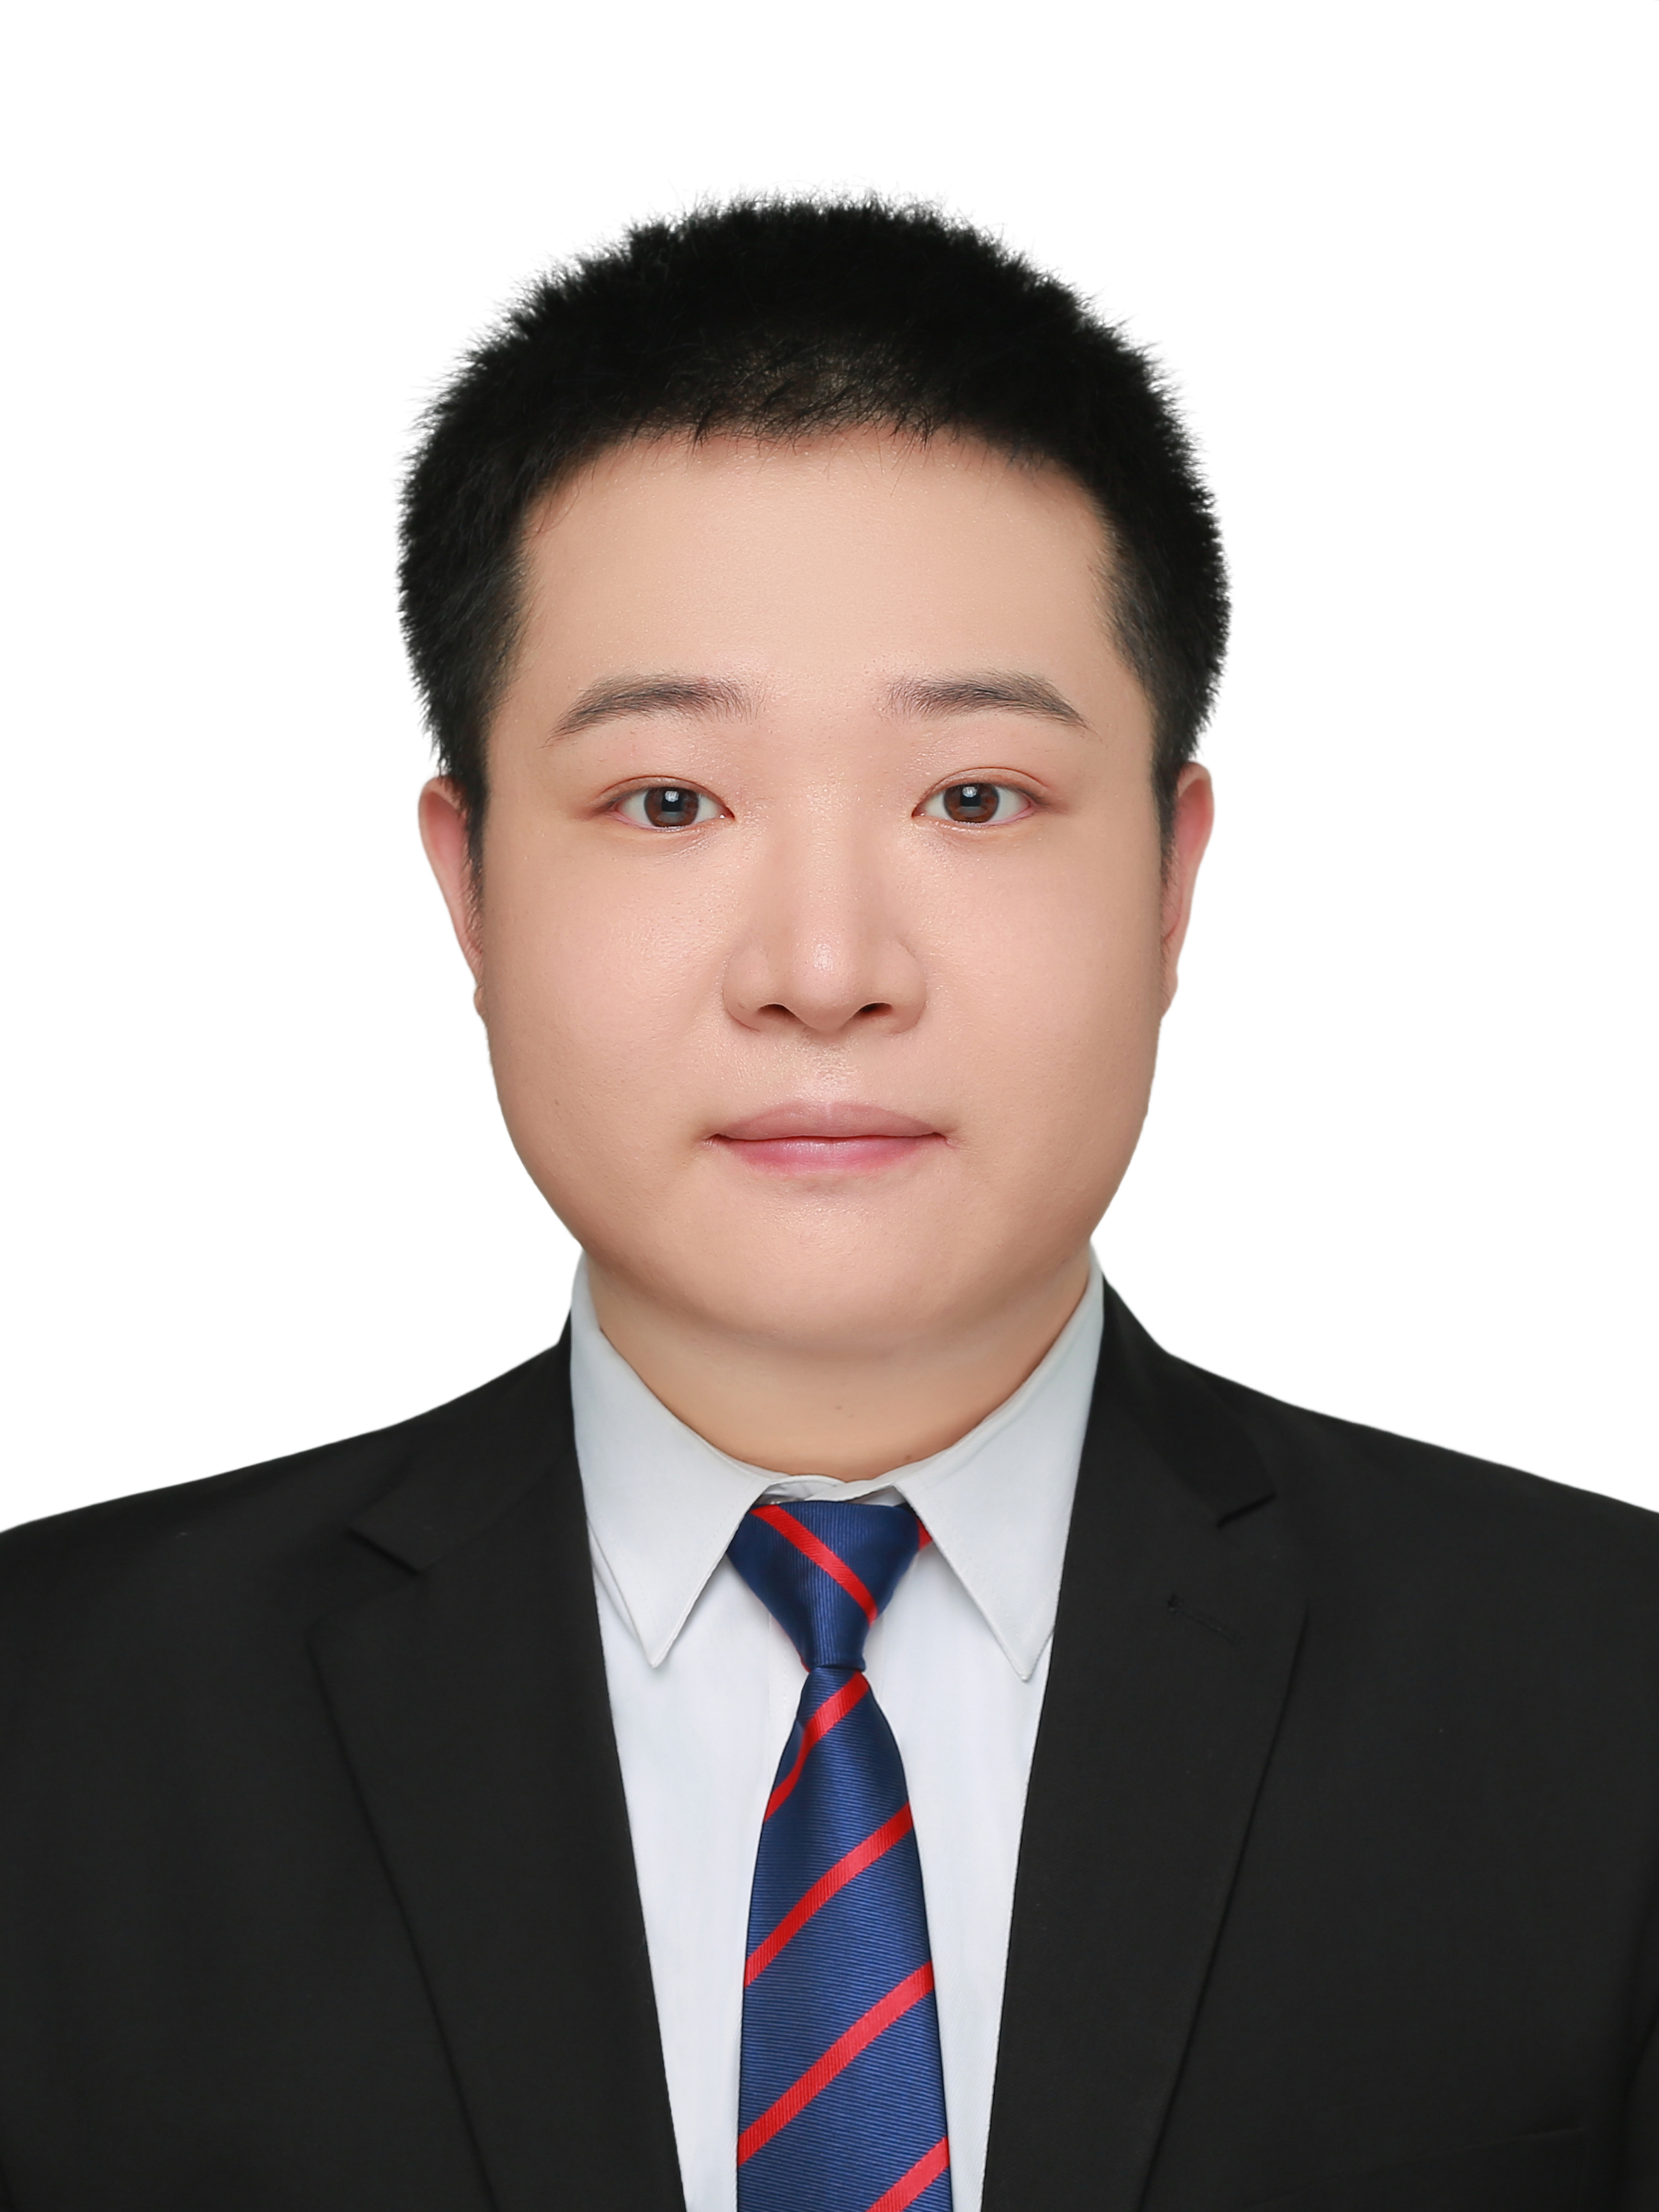
\includegraphics[width=1in,height=1.25in,clip,keepaspectratio]{author/ChenWei}}]{Chen Wei}
	received the bachelor’s degree in electronic and information engineering from Shandong University, Jinan, China in 2018. He is currently pursuing the Ph.D. degree in microelectronics and solid-state electronics with Shenzhen Graduate School, Peking University. His current research interest is the reliability design of 2.5D/3D ICs.
\end{IEEEbiography}

\begin{IEEEbiography}[{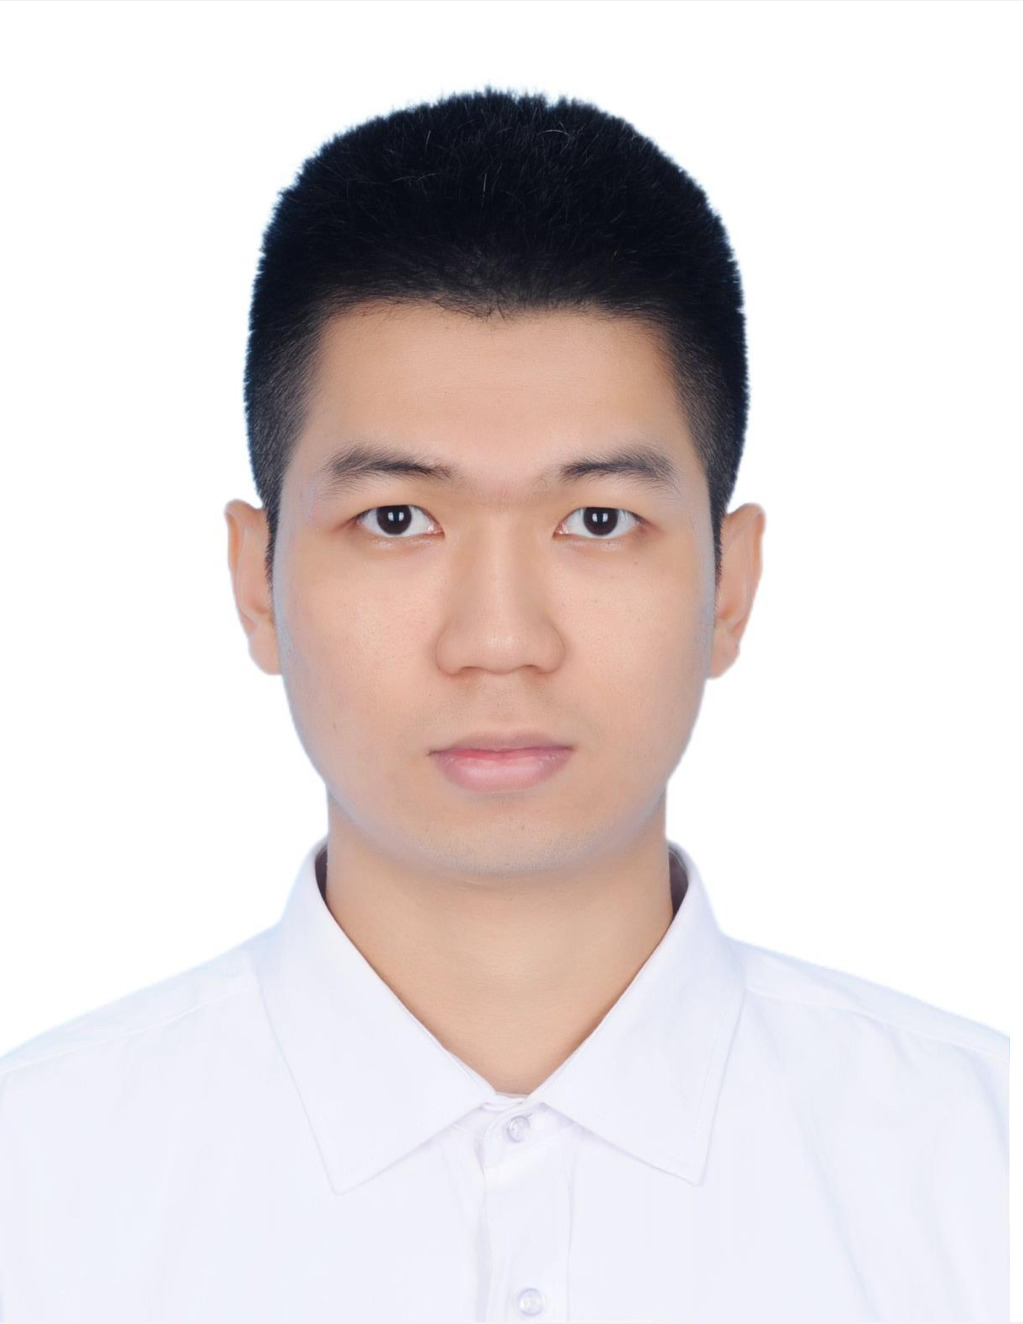
\includegraphics[width=1in,height=1.25in,clip,keepaspectratio]{author/HuanYang}}]{Huan Yang}
	received the B.E. degree in Microelectronics Science and Engineering from  Shenzhen University, Shenzhen, China, in 2022. He is now pursuing the Ph.D. degree in Integrated Circuit Science and Engineering with Peking University Shenzhen Graduate School, Shenzhen, China. His current research interests include the reliability of 3D ICs and SoC designs.
\end{IEEEbiography}

\begin{IEEEbiography}[{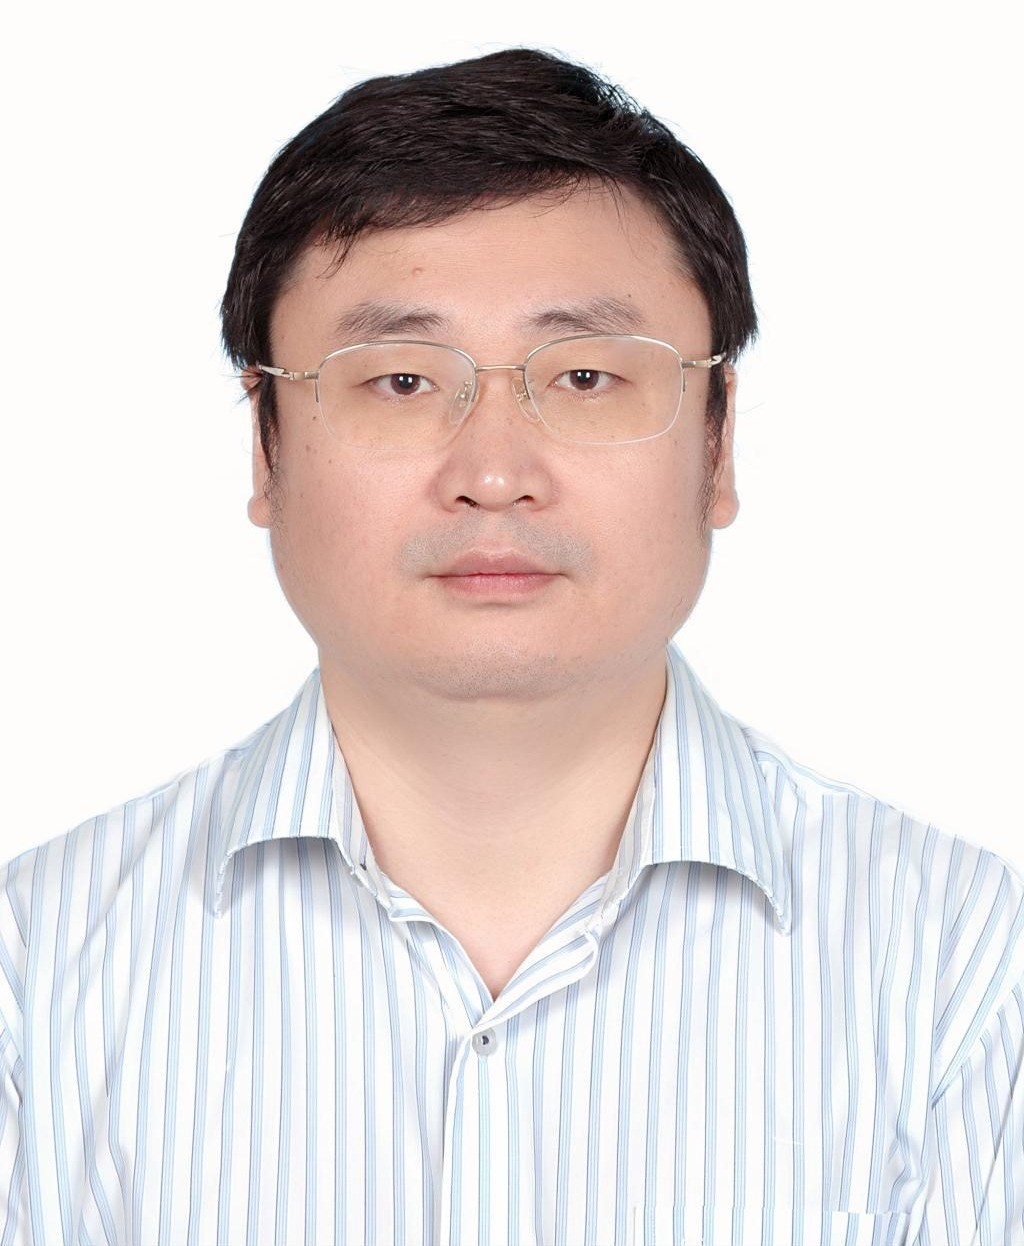
\includegraphics[width=1in,height=1.25in,clip,keepaspectratio]{author/XiaoleCui}}]{Xiaole Cui}
	received the B.Sc. degree in communication engineering from Xidian University, Xi’an, China, the M.Sc. degree in computer engineering from Xi'an Institute of Microelectronics, Xi’an, China, and the Ph.D. degree in system engineering from Beihang University, Beijing, China, in 1997, 2000, and 2004, respectively. He is currently a professor in Shenzhen Graduate School, Peking University, Shenzhen, China. His research interests include VLSI design and testing, reliability and safety of electronic systems, and dependable computing. 
\end{IEEEbiography}

\begin{IEEEbiography}[{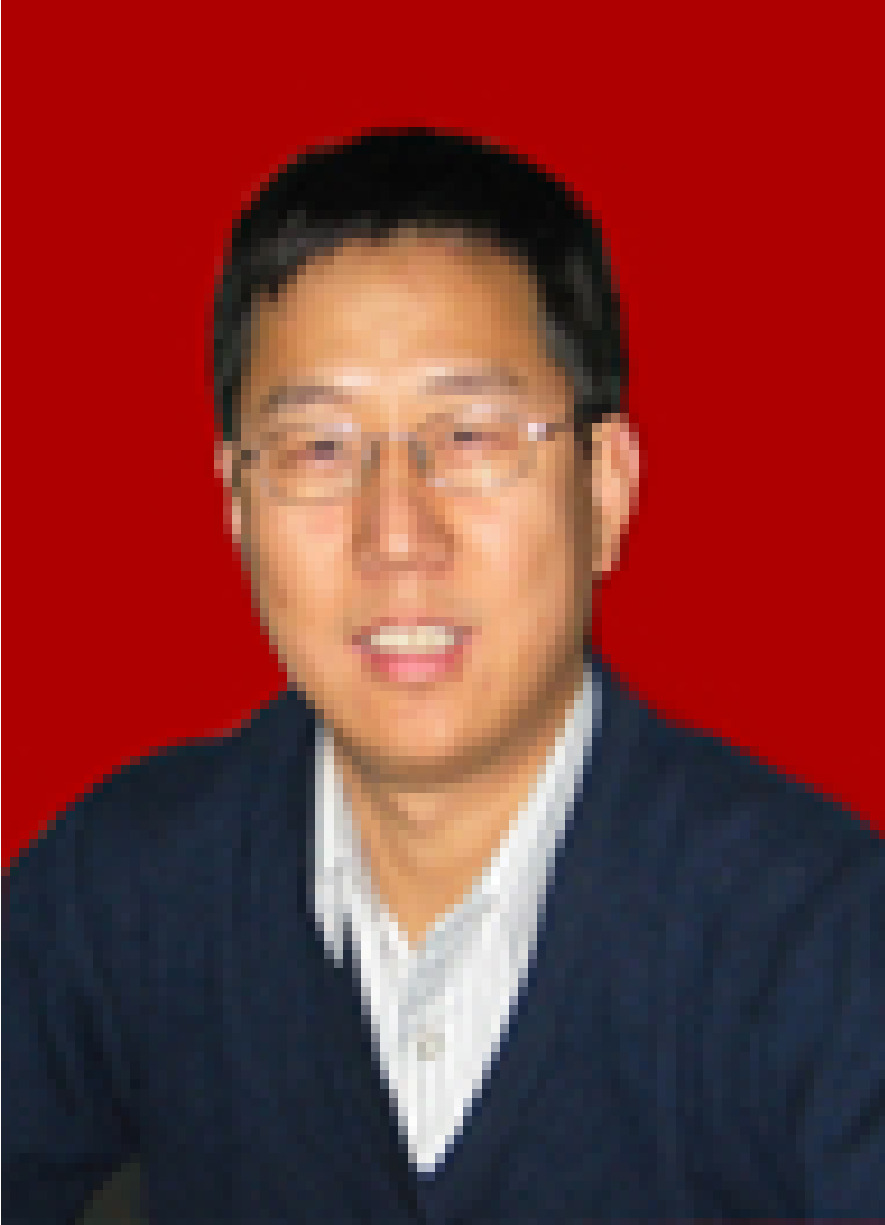
\includegraphics[width=1in,height=1.25in,clip,keepaspectratio]{author/XingZhang}}]{Xing Zhang}
	was born in Shandong, China. He	received the B.S. degree in physics from Nanjing University, Nanjing, China, in 1986, and the M.S. and Ph.D. degrees in microelectronics from the Shaanxi Microelectronics Institute, Shaanxi, China, in 1989 and 1993, respectively. He is currently a Professor with Peking University. He has authored or coauthored three books and more than 200 research papers. His current research interests include the physics and novel structures of nano-scaled MOS devices, model and simulation, CMOS IC design, and process technology.
	
\end{IEEEbiography}


\vfill

\end{document}


